%-----------------------------------------------------------------------------
%
%               Template for sigplanconf LaTeX Class
%
% Name:         sigplanconf-template.tex
%
% Purpose:      A template for sigplanconf.cls, which is a LaTeX 2e class
%               file for SIGPLAN conference proceedings.
%
% Guide:        Refer to "Author's Guide to the ACM SIGPLAN Class,"
%               sigplanconf-guide.pdf
%
% Author:       Paul C. Anagnostopoulos
%               Windfall Software
%               978 371-2316
%               paul@windfall.com
%
% Created:      15 February 2005
%
%-----------------------------------------------------------------------------


\documentclass[article,reprint]{sigplanconf}

% The following \documentclass options may be useful:
%
% 10pt          To set in 10-point type instead of 9-point.
% 11pt          To set in 11-point type instead of 9-point.
% authoryear    To obtain author/year citation style instead of numeric.

\usepackage{amsmath,amssymb,amsthm}
\usepackage{color,graphicx,subfigure}
\usepackage{algpseudocode}
\algtext*{EndWhile}% Remove "end while" text
\algtext*{EndIf}% Remove "end if" text
\algtext*{EndFor}% Remove "end for" text
\usepackage{qtree}
\usepackage{epsfig,epstopdf}
\usepackage{multirow}
\usepackage{listings}
\usepackage{url}

\newcommand{\shrink}{\vspace*{-2ex}}

\newcommand{\XJ}[1]{\textcolor{red}{[XJ: #1]}}
\newcommand{\KZ}[1]{\textcolor{blue}{[KZ: #1]}}
\newcommand{\RY}[1]{\textcolor{blue}{[RY: #1]}}

\newcommand{\nat}{\mathbb{N}}

\newcommand{\cm}{\textbf{cm}}
\newcommand{\cu}{\textbf{cu}}
\newcommand{\dm}{\mathcal{DM}}
\newcommand{\mkstore}{\Delta_0}
\newcommand{\alltype}{\mathcal{T}}
\newcommand{\allop}{\mathcal{P}}
\newcommand{\allstore}{\mathcal{D}}
\newcommand{\dtrans}{\psi}
\newcommand{\dptype}{\tau_p}
\newcommand{\dstype}{\tau_d}
\newcommand{\alluniv}{\mathcal{U}}
\newcommand{\allexpr}{\mathcal{E}}

\newcommand{\emptytop}{U_\emptyset}

\newcommand{\typeof}[1]{\tau\ldbrack #1\rdbrack}

% transition arrows
\newcommand{\uto}{\longrightarrow}
\newcommand{\gto}{\hookrightarrow}

\newcommand{\gmerge}{merge}%{\textsc{Merge}}
\newcommand{\gpaste}{paste}%{\textsc{Paste}}

\newcommand{\snapshot}{\mathcal{S}}%{\textsc{\color{red}Snapshot}}

\newcommand{\ldbrack}{[\hspace{-0.5mm}[}
\newcommand{\rdbrack}{]\hspace{-0.5mm}]}
\newcommand{\lbb}{\{\hspace{-0.7mm}|}
\newcommand{\rbb}{|\hspace{-0.7mm}\}}

\newcommand{\compact}[1]{\!\!#1\!}
\newcommand{\bk}{\hspace{-1mm}}

\newtheorem{theorem}{Theorem}
\newtheorem{lemma}{Lemma}
\newtheorem{proposition}{Proposition}
\newtheorem{corollary}{Corollary}
\newtheorem{definition}{Definition}
\newtheorem{property}{Property}
\newtheorem{axiom}{Axiom}
\newtheorem{example}{Example}

\newcommand{\figref}[1]{Figure \ref{#1}}
\newcommand{\tabref}[1]{Table \ref{#1}}
\newcommand{\eqnref}[1]{Eq. (\ref{#1})}

\newcommand{\nl}{\vspace*{3mm}}

\makeatletter
 \let\@copyrightspace\relax
\makeatother

\lstset{
  captionpos=b,
  tabsize=2,
  numbers=left,
  numberstyle=\tiny,
  numbersep=5pt,
  breaklines=true,
  showstringspaces=true,
  basicstyle=\scriptsize\ttfamily,
  frame=none,
  emph={label},
  escapechar=| % Escape to LaTeX between |...|
}

\begin{document}

\setlength{\abovedisplayskip}{3pt}
\setlength{\belowdisplayskip}{2pt}

\conferenceinfo{WXYZ '05}{date, City.}
\copyrightyear{2005}
\copyrightdata{[to be supplied]}

\titlebanner{banner above paper title}        % These are ignored unless
\preprintfooter{short description of paper}   % 'preprint' option specified.

%\title{A Calculus for Speculative Non-determinism}
\title{Speculative Nondeterminism}
%\subtitle{Subtitle Text, if any}

\authorinfo{Xiao Jia \and Kenny Q. Zhu}
           {Shanghai Jiao Tong University}
           {\{xjia,kzhu\}@cs.sjtu.edu.cn}
\authorinfo{Joxan Jaffar \and Roland H.C. Yap}
           {National University of Singapore}
           {\{joxan,ryap\}@comp.nus.edu.sg}

\maketitle

\begin{abstract}
We propose a new programmable concurrency control framework called
speculative nondeterminism for real time,
``open'' and distributed agents. By open, we mean the agent programs
are independent and are not necessarily constrained to operate
in a particular fashion, and they may join the system at arbitrary times.
In this framework,
agent programs execute concurrently and affect each other through
a centralized store which represents shared resources.
%There is no direct communication among the agents.
%Because a sequential agent maybe blocked due to resource constraints
%in the store,
The framework allows the agent to speculate against the future by multiple
exclusive choices that encode different strategies to achieve its goals.
As the choices are exclusive, each choice from the same agent
executes in isolation from the other, however,
agents still interact with each other through the store.
The benefit of speculation is that unlike other concurrency frameworks,
the combinatorial-choice models more possibilities and
this improves the chances of successful outcomes in a system with interacting agents.
% The choices from the same agent are meant to be executed in
% isolation from each other because they may update the store in different ways.
% Only one successful choice becomes the eventual reality. When multiple
% agents each specifies some choices, the system creates
% many stores and thus runtime environments to represent the
% different combinations of choices. We argue that combinatorial choices
% improve the likelihood of successful program completion and
% thus improve the overall system throughput.
The framework also allows the agent to specify when and where
it wants to commit to a particular choice
and thus control the space of choices and reclaim valuable computation resources.
This paper gives the formal operational semantics of speculative nondeterminism,
and presents a prototype implementation of the framework along with some
preliminary evaluation results.
\end{abstract}

%\category{CR-number}{subcategory}{third-level}

%\terms
%term1, term2

\keywords
speculation, concurrency, nondeterminism, agents

%\IEEEraisesectionheading{
% %\IEEEraisesectionheading{
% %\IEEEraisesectionheading{
% \input{intro}
\section{Introduction}\label{sec:intro}
 %}
% \section{Introduction}\label{sec:intro}

% \begin{enumerate}
% \item Motivation: application scenarios (with 1-2 running examples);
% \item Characteristics of the data sources and their challenges;
% \item Briefly introduce previous approaches to extract information 
% from images including setting the document zone, and their limitations.
% \item General flow of our approach (may give a diagram here)
% \end{enumerate}
% scenary

Due to ever evolving hardware and software, many medical images
such as electro-cardio graphs (ECGs), X-ray or ultrasound images  
are directly printed and stored in hard copy formats. 
% \KZ{Insert 4 example images here.}
%Examples are shown in \figref{fig:medicalImages}. 
% These images often contain a mix of graphics and text, which
% include parameter settings of the hardware, test measurements or simple
% diagnosis. 
These images often contain a mix of graphics and text, which 
include technical settings of the hardware used, test measurements or simple diagnoses.
Recently, there has been a growing demand for digitizing such 
medical information from paper media sources, especially legacy ones, or patients who want to keep track of these documents by themselves digitally. 
Apart from scanning the graphics into a digital format, extracting 
the semi-structured textual information is also an important part of
building electronic medical records for patients. 

%\begin{figure}[!htb]
%\centering
%\subfloat[ECG]{
%\label{fig:medicalimage:ecg}
%\epsfig{file=figure/17_ori.eps, width=0.4\columnwidth}
%}
%% \hfill
%\subfloat[MRI]{
%	\label{fig:medicalimage:mrt}
%	\epsfig{file=figure/MRI.eps, width=0.4\columnwidth}
%}
%\\
%\subfloat[X-RAY]{
%\label{fig:medicalimage:xray}
%\epsfig{file=figure/X-RAY.eps, width=0.4\columnwidth}
%}
%%\hfill
%\subfloat[EEG]{
%\label{fig:medicalimage:eeg}
%\epsfig{file=figure/EEG.eps, width=0.4\columnwidth}
%}
%\caption{Examples of Medical Images}
%\label{fig:medicalImages}
%\end{figure}

Optical character recognition (OCR)  \cite{mori1992historical,smith2007overview} is 
a traditional technique used to turn images of printed text into machine encoded
text. It is well researched and performs well on plain text 
documents such as novels and reports, for a variety of languages. 
%For example, Tesseract, which is one of 
%the most popular open source multilingual recognizers, logs an error 
%rate of 3.72\% for English words and 3.77\% for simplified 
%Chinese characters\cite{smith2009adapting}. 
%Google Books \cite{googlebooks} and Gutenberg \cite{gutenberg} are
%projects which have scanned a large number of paper books into text for free and open
%access. These projects made exclusive use of OCR for this conversion and 
%achieved high accuracy \cite{vincent2007google} \cite{lebert2008project}. 
% 99\% for Gutenberg project \cite{lebert2008project}. 
% \KZ{Give the accuracy of google and gutenberg if available.}


\begin{figure}[th]
\centering
\epsfig{file=figure/17_b.eps, width=0.8\columnwidth}
\caption{An ECG image with text area (red circle) of interest.}
\label{fig:ecgexample2}
\end{figure}

For a semi-structured medical image, such as 
\figref{fig:ecgexample2}, we would like to extract the attribute-value 
pairs (e.g., {\em Vent. rate = 63 bpm}) and possibly other values such as
date ({\em 18-Nov-2010}) and time ({\em 9:13:02}) since those values endow us with lots of information about the patient. 
Existing OCR software cannot extract such structured information in a straightforward 
fashion, 
but instead it produces rather convoluted results from the whole image, 
similar to those in \figref{fig:ocrre}, which was produced by Tesseract, 
a popular multi-lingual recognizers. 
% \KZ{Maybe include the x-y coordinate info in the output as well?}  

\begin{figure}[th]
\centering
\scriptsize
\begin{verbatim}
<p class="ocr_par" title="box 263 33 444 119">
   <span class="ocr_l" title="box 264 33 336 45">
       <span class="ocrx_w" title="box 264 33 299 45">Vcnt.</span> 
       <span class="ocrx_w" title="box 308 34 336 45">rule</span> 
   </span>
   <span class='ocr_l'>
       <span class="ocrx_w" title="box 264 51 283 64">PR</span> 
       <span class="ocrx_w" title="box 291 51 346 64">Interval</span> 
       <span class="ocrx_w" title="box 389 52 411 64">140</span> 
       <span class="ocrx_w" title="box 420 55 439 64">ms</span> 
   </span>
   ...
   </span>
</p>
<p class="ocr_p" dir="ltr">
   <span class="ocr_l">
       <span class="ocrx_w" title="box 396 33 411 45">53</span> 
       <span class="ocrx_w" title="box 420 33 449 48">bpm</span> 
   </span>
</p>
\end{verbatim}
\caption{Snippet OCR results in XML, input to our framework.}
\label{fig:ocrre}
\end{figure}


%\input{xmlre1}

%However, OCR alone does not work well on semi-structured text and hence
%can't be directly used for information extraction from the aforementioned
%medical images. \KZ{Give the reason here, perhaps because OCR models are
%largely Markov based? So semi-structured data breaks the flow of text.}
%When a medical image is input to an ordinary OCR software, the spatial 
%information of the text components is often lost or mixed with noises
%and errors.
%%The reason is OCR converts the whole images into text data, in which 
%%useful information often mix with noises and errors. 
%In this paper, we would like to extract the attribute-value pairs
%and possibly other values from \figref{fig:ecgexample1} 
%and \figref{fig:ecgexample2}. 
%% or medical ultrasonography report. 
%Such images contain lots of non-textual information or noises.

% example & ref
%\begin{figure}[ht]
%\centering
%\epsfig{file=figure/46.eps, width=0.8\columnwidth}
%\caption{ECG Images From Printer1}
%\label{fig:ecgexample1}
%\end{figure}

% \begin{figure}[ht]
% \centering
% \subfloat[Printer1]{
% \label{fig:ecgexample:a}
% \epsfig{file=figure/46.eps, width=0.48\columnwidth}
% }
% \hfill
% \subfloat[Printer2]{
% \label{fig:ecgexample:b}
% \epsfig{file=figure/17.eps, width=0.48\columnwidth}
% }
% \caption{ECG images from two different printers}
% \label{fig:ecgexample}
% \end{figure}

Also, errors in the OCR text \cite{darwish2007error,taghva1996evaluation} will greatly affect the effectiveness 
of other related tasks. Much work has been done to improve the performance of the OCR\cite{kolak2003generative,cesarini1998informys}. However, there are still a number of significant challenges involved in extracting the information from medical images or OCR results in XML form. 

% First, medical images differ from pure text document in that them have 
% layout information. 
First, medical images differ from pure text documents in that 
they contain layout information.
Although most current OCR engines attempt to reproduce the physical 
layout of the text units, 
%(along with X-Y coordinates) and store them 
%in a special format such as XML 
% (\KZ{Better in the previous example})
such spatial
information is approximate and sometimes inaccurate, which is why neighboring
text blocks in \figref{fig:ecgexample2}, such as ``Vent. Rate'' and
``63 bpm'' were not automatically combined into the same XML block, but were 
rather far apart (shown in two different ``classes'') in \figref{fig:ocrre} made by OCR softwares. 
%Even for images produced by the same ECG printer, 
%the XML results can still be very different as 
The spatial layout is sensitive to many factors, such as accidental spots 
on the prints, color and contrast, or the angle of the camera. 
%In this case, solutions for other application domains, for example, the web, 
%are not well suited for information extraction from printed documents \cite{bartoli2014semisupervised}. With such inaccurate
%layout information produced by OCR,
%it is not easy to write a simple wrapper program to extract useful
%data from images, even if the images come from the same printer. 

%Writing a wrapper for each
%individual image would be tedious and counter-productive. Therefore,
%a mechanism that makes use of the spatial locality of the 
%text units in the image and 
%accommodates slight variations in the spatial layout would make the extraction
%more accurate and fault-tolerant.

%For example, \figref{fig:ocrre} is the simplified OCR results for the ECGs in 
%\figref{fig:ecgexample1} and \figref{fig:ecgexample2}. The results are in the XML format and have attritube named {\em class} 
%for layout information. Although these two images share similar format. 
%OCR engine generates different results in that it splits elements that 
%should be in the same line into two lines in the second example. 
%XML is sensitive to the layout results so it's hard to tolerate 
%all the layout results. 
%
% example check the term
% layout of ocr results can be restore, so why OCR engine don't restore the results 
% using the similar methods as we do?
% or the way we handle the layout problem is quite simple

% Delete for TIP
% Second, exiting OCR engines make heavy use of Markov properties such as n-grams
% since they primarily target the transformation of large body of text 
% \cite{kolak2003generative}. 
% % \KZ{Needs some refs here.}
% Unfortunately, the semi-structured texts in medical images are often 
% short and not even written in complete sentences, thus breaking Markov assumption. To make
% matters worse, medical images contain scientific language, which may be
% very different from the training corpora of these OCR engines.
% This explains why we see errors like ``Vcnt'' and ``rule'' 
% in \figref{fig:ocrre}. 
% %can't guarantee a perfect performance, which means 
% %there are errors and noises in the OCR results.
% %Many of them due to the fact that the data are no longer long, continous
% %sentences, thus breaking the Markov assumption made by many OCR algorithms. 
% %In \figref{fig:ocrresub:b}, ``Vent." is misrecognized as ``Vcnt.". 
% Without sufficient contextual information, OCR may also misrecognize a 
% digit as an alphabetic character, or as another similar digit. 
% Furthermore, the mix of text with images and formatting
% lines often confuses the OCR engine, which is more biased toward full
% text images.
% Exact pattern matching, as used in
% traditional information extraction, doesn't work with such noisy OCR output
% as it doesn't tolerate noises or errors in text. 
% %It's hard to autocorrect these errors 
% %because image quality is the most important affecting factor. 
% %The text we are processing can be full of no meaning words or 
% %strange numbers. 
% A fuzzy matching strategy is more desirable in this case. 
% % example, what are the traditional IEs

Second, there are many types of medical images, resulting from a variety of
medical tests. Different equipments for the same test can produce vastly 
different images. Writing individual extraction wrappers 
for the OCR outputs of all these formats is tedious and inefficient, 
and difficult for non-programmers.
%not to mention that there are significant programming barriers for 
%writing these wrappers, especially for the medical professionals who are the
%end users of these extraction results. 
%A more user-friendly approach enabling users to specify such extraction requirements would be preferred. 
%There are various kinds of medical images, such as electrocardiograph report, 
%medical ultrasonography report, etc. 
%However the basic measures for each type of medical test (e.g., ECG), 
%are very similar from machine to machine. Only the layouts are 
%different. 
% example medical images

Finally, most off-the-shelf OCR programs are pre-trained with specific 
recognition models, which may not be suitable for the extraction of 
%medical images.
%Furthermore, changes in imaging equipment technology over time may produce 
%different formats, layout, or terminology, rendering existing OCR models 
%obsolete. 
Re-training the models requires a large amount of labeled data, which may
not be available. 
%Incremental training as more labeled data arrives
%is currently not supported by any OCR product.    

%There have been some limited attempts to address some of the above challenges. 
%One solution is a plugin of an OCR program that allows the user to specify 
%target zones of interest in the image to be extracted. The zones specified for
%one image can be applied to images with slight variations by adjusting against
%a fixed reference point that is supposed to exist in all these images.
%% \KZ{I think the problem is not so much with the zones, because we also
%% have zones, but rather with the reference point.}
%% \JY{}
%% example products
%% http://www.square-9.com/automated-data-extraction-optical-character-recognition
%The problem with this solution is its high reliance on the OCR zones  
%established by the user. The performance of the results is affected by the 
%accuracy of the zones. If the zones are too big, the results will be full of 
%noise. If the zones are too small, results will miss something. 
%
%Another solution involves using the page layout analysis technique. The page layout 
%analysis technique is used to determine where the text 
%resides on a page \cite{o1993document}, 
%% \KZ{This page layout analysis approach is not clearly described. I don't understand after reading this paragraph.}
%% By using page layout analysis technique, the hierarchy of physical components 
%% can be generated and to match with the hierarchy of logical components, which 
%% is predefined. 
%this includes identifying and categorizing the 
%regions of interest in the scanned image of a text document. 
%Typically, the first step is to segment text zones from 
%non-textual zones and arrange them in their original order. 
%Then in order to analyze the logical roles of the text zones 
%(titles, captions, footnotes, etc.), logical layout analysis 
%is used for labeling the semantics of the text zones.
%Generally, page layout analysis is used for documents. The problem with applying 
%such a technique on medical images is that it creates so much noises 
%that performance is ultimately affected. 
%For medical imaging reports like ECG, useful information is often 
%found in the small components of the image, while most of the images are 
%read as noises. 
% check paper and more description, weakness, ref

%In this paper, 
%we propose a spatial data description language, which borrows its syntax from
%PADS \cite{fisher+:pads}, an ad hoc data processing language, 
%for describing semi-structured data in medical images. 
%% ref
%We call this language OCR description language, or ODL. 
%ODL is designed for extracting and parsing semi-structured text data 
%from images. We believe that  information extraction from those data in ODL form may be much easier than extracting information from rough data or data in XML form, which means that our preprocessing part proves to be necessary.
%%An example ODL description for the image in 
%%\figref{fig:ecgexample2} is shown in 
%%\figref{fig:description}. \KZ{Make this description two column, and give
%%some brief explanation of this description here.} 
%%The parsing result of this description is shown
%%in \figref{fig:parsing result}. \KZ{Give some explanation of the results,
%%otherwise don't show the result here. E.g., you need to explain what F, E, etc.
%%mean. You want to say that even though rate has been recognized as rule,
%%the bpm value was still extracted (but still wrong!).}
%% \KZ{I removed the preprocessing part, cos it's not important. Talk about it in
%% discussion sec.}
%%The our approach starts by preprocessing the images for text results.
%To use this framework, the user first describes the components in the image
%that he or she is interested in extracting. This includes constant strings
%and variables of different data types.   
%ODL allows the user to specify the approximate spatial layout and constraints on
%the data, e.g., integers within 
%a certain range, real numbers with certain decimal points, etc. 
%%This information is then as the key component in our fuzzy matching strategy. 
%The system then automatically generates a parser for these medical images.
%This parser uses the output XML from OCR with spatial information as an input, 
%and outputs a data structure with values extracted for each variables
%in the description, unless there is an unrecoverable error during the parsing process.
%In addition, approximate layout information and constraints are used in parsing process 
%to tolerate noises and small format variations in the input images. 
%%Specifically, this method could be called fuzzy matching, meaning that more candidates could be saved after the parsing process.  It's obvious that we may have a higher probability to obtain the accurate result if more candidates are kept so that fuzzy match should be used properly in our system.
%%An autogenerated parser based on the ODL description can release us from 
%%repetitive work. In this way, we turn the task of writing complex parsers 
%%into describing information on images.
%
%
%When users process many images of the same format, the system 
%automatically discovers parsing errors given the current model and 
%prompts the user to manually correct some of the frequent and prominent
%errors, which effectively serves as an online labeling function. 
%These incrementally labeled data are then used to update the parsing model. 


%It should be emphasized that the incremental learning model is very important in our whole system. Incremental learning is a machine learning paradigm where the learning process takes place whenever we have new examples or data added to our baisc data set, leading to a most striking difference between incremental learning and traditional machine learning: it does not assume the availability of a sufficient training set before the learning process. What incremental learning in our system is really impressive: it does not require a relatively good and stable training set at first time. In fact, it could improve the parsing result with even relatively rough training sets at first by absorbing new data or corrective information as time passes in dynamic systems. Besides, the process would be very effective when there are some new images coming in since training process would not learn from scratch, which might waste time and computation resource.

%At last, we propose an incrementally human correction framwork which can 
%make the best use of human correction to handle the misrecognition problem. 
% Base on our experiments on about 500 real life ECG images, 
% our approach achieves p1 and p2 after p3 times human correction. 
% experimental results

% \begin{figure}[h]
% \begin{lstlisting}
% Oenum str_month_t{
% 	"Jan", "Feb", "Mar", "Apr",
% 	"May", "Jun", "Jul", "Aug",
% 	"Sept", "Oct", "Nov", "Dec"
% };

% Ounion month_t{
% 	Oint(1,12)	num;
% 	str_month_t	str;
% };

% Ostruct time_t{
% 	Oint(1,31)	day;
% 	"-";
% 	month_t	month;
% 	"-";
% 	Oint	year;
% };

% Ostruct triple_t{
% 	"Vent.";
% 	hskip(\s)	skip1;
% 	"rate";
% 	Oint x;
% 	"bpm";
% 	vskip(\n)	skip2;
% };

% Oscource Ostruct entry_t{
% 	time_t(<-,-,-,0.3l>) t;
% 	triple_t(<0.1w,-,0.5w,->) d;
% };
% \end{lstlisting}
% \caption{Description}\label{fig:description}
% \end{figure}


In order to solve above problems, We design a system which makes three main contributions:
\begin{enumerate}
\item Based on some previous work on data description language \cite{lamport1986document,taft1999post,fisher+:pads},we design a new declarative spatial data description language called \textit{OCR description language}, or ODL,
which allows users to specify spatial and data constraints in medical 
images(\secref{sec:syntax});
\item We propose a noise-tolerant parser which takes OCR results
the ODL description as input and outputs a data structure with values 
extracted for each variables in the description (\secref{sec:semantics});
\item We propose an incremental manual correction 
framework\cite{von2008recaptcha,zhu2012learnpads++}, which 
takes advantage of user corrections  and improves the productivity
significantly (\secref{sec:correction}).
%To be more specific, the framework improves the traditional machine learning methods by using a incremental learning process to avoid starting from scratch when we are trying to apply human corrections in the system. That means the framework would be more effective than most corrective systems.
\end{enumerate}


\section{Introduction}\label{sec:intro}
 %}
% \section{Introduction}\label{sec:intro}

% \begin{enumerate}
% \item Motivation: application scenarios (with 1-2 running examples);
% \item Characteristics of the data sources and their challenges;
% \item Briefly introduce previous approaches to extract information 
% from images including setting the document zone, and their limitations.
% \item General flow of our approach (may give a diagram here)
% \end{enumerate}
% scenary

Due to ever evolving hardware and software, many medical images
such as electro-cardio graphs (ECGs), X-ray or ultrasound images  
are directly printed and stored in hard copy formats. 
% \KZ{Insert 4 example images here.}
%Examples are shown in \figref{fig:medicalImages}. 
% These images often contain a mix of graphics and text, which
% include parameter settings of the hardware, test measurements or simple
% diagnosis. 
These images often contain a mix of graphics and text, which 
include technical settings of the hardware used, test measurements or simple diagnoses.
Recently, there has been a growing demand for digitizing such 
medical information from paper media sources, especially legacy ones, or patients who want to keep track of these documents by themselves digitally. 
Apart from scanning the graphics into a digital format, extracting 
the semi-structured textual information is also an important part of
building electronic medical records for patients. 

%\begin{figure}[!htb]
%\centering
%\subfloat[ECG]{
%\label{fig:medicalimage:ecg}
%\epsfig{file=figure/17_ori.eps, width=0.4\columnwidth}
%}
%% \hfill
%\subfloat[MRI]{
%	\label{fig:medicalimage:mrt}
%	\epsfig{file=figure/MRI.eps, width=0.4\columnwidth}
%}
%\\
%\subfloat[X-RAY]{
%\label{fig:medicalimage:xray}
%\epsfig{file=figure/X-RAY.eps, width=0.4\columnwidth}
%}
%%\hfill
%\subfloat[EEG]{
%\label{fig:medicalimage:eeg}
%\epsfig{file=figure/EEG.eps, width=0.4\columnwidth}
%}
%\caption{Examples of Medical Images}
%\label{fig:medicalImages}
%\end{figure}

Optical character recognition (OCR)  \cite{mori1992historical,smith2007overview} is 
a traditional technique used to turn images of printed text into machine encoded
text. It is well researched and performs well on plain text 
documents such as novels and reports, for a variety of languages. 
%For example, Tesseract, which is one of 
%the most popular open source multilingual recognizers, logs an error 
%rate of 3.72\% for English words and 3.77\% for simplified 
%Chinese characters\cite{smith2009adapting}. 
%Google Books \cite{googlebooks} and Gutenberg \cite{gutenberg} are
%projects which have scanned a large number of paper books into text for free and open
%access. These projects made exclusive use of OCR for this conversion and 
%achieved high accuracy \cite{vincent2007google} \cite{lebert2008project}. 
% 99\% for Gutenberg project \cite{lebert2008project}. 
% \KZ{Give the accuracy of google and gutenberg if available.}


\begin{figure}[th]
\centering
\epsfig{file=figure/17_b.eps, width=0.8\columnwidth}
\caption{An ECG image with text area (red circle) of interest.}
\label{fig:ecgexample2}
\end{figure}

For a semi-structured medical image, such as 
\figref{fig:ecgexample2}, we would like to extract the attribute-value 
pairs (e.g., {\em Vent. rate = 63 bpm}) and possibly other values such as
date ({\em 18-Nov-2010}) and time ({\em 9:13:02}) since those values endow us with lots of information about the patient. 
Existing OCR software cannot extract such structured information in a straightforward 
fashion, 
but instead it produces rather convoluted results from the whole image, 
similar to those in \figref{fig:ocrre}, which was produced by Tesseract, 
a popular multi-lingual recognizers. 
% \KZ{Maybe include the x-y coordinate info in the output as well?}  

\begin{figure}[th]
\centering
\scriptsize
\begin{verbatim}
<p class="ocr_par" title="box 263 33 444 119">
   <span class="ocr_l" title="box 264 33 336 45">
       <span class="ocrx_w" title="box 264 33 299 45">Vcnt.</span> 
       <span class="ocrx_w" title="box 308 34 336 45">rule</span> 
   </span>
   <span class='ocr_l'>
       <span class="ocrx_w" title="box 264 51 283 64">PR</span> 
       <span class="ocrx_w" title="box 291 51 346 64">Interval</span> 
       <span class="ocrx_w" title="box 389 52 411 64">140</span> 
       <span class="ocrx_w" title="box 420 55 439 64">ms</span> 
   </span>
   ...
   </span>
</p>
<p class="ocr_p" dir="ltr">
   <span class="ocr_l">
       <span class="ocrx_w" title="box 396 33 411 45">53</span> 
       <span class="ocrx_w" title="box 420 33 449 48">bpm</span> 
   </span>
</p>
\end{verbatim}
\caption{Snippet OCR results in XML, input to our framework.}
\label{fig:ocrre}
\end{figure}


%% \begin{figure}[ht]
% \centering
% \subfigure[]{
% \label{fig:subfig:a}
% \begin{minipage}[b]{0.2\textwidth}
%\newsavebox{\firstlisting}
%\begin{lrbox}{\firstlisting}% Store first listing
%\begin{lstlisting}
%<p class='ocr_par' dir='ltr'>
%   <span class='ocr_line' id='line_2'>
%       <span class='ocrx_word' id='word_6'>Vent.</span>
%       <span class='ocrx_word' id='word_7'>rate</span>
%       <span class='ocrx_word' id='word_8'>65</span>
%       <span class='ocrx_word' id='word_9'>bpm</span>
%   </span>
%   <span class='ocr_line' id='line_3'>
%       <span class='ocrx_word' id='word_14'>PR</span>
%       <span class='ocrx_word' id='word_15'>interval</span>
%       <span class='ocrx_word' id='word_16'>162</span>
%       <span class='ocrx_word' id='word_17'>ms</span>
%   </span>
%    ...
%</p>
%\end{lstlisting}
%\end{lrbox}
% \end{minipage}
% }
% \hspace[1in]
% \subfigure[]{
% % \label{fig:subfig:b}
% % \begin{minipage}[b]{0.2\textwidth}
\newsavebox{\secondlisting}
\begin{lrbox}{\secondlisting}
% \tiny
\begin{lstlisting}[basicstyle=\tiny,]
<p class="ocr_par" title="box 263 33 444 119">
   <span class="ocr_l" title="box 264 33 336 45">
       <span class="ocrx_w" title="box 264 33 299 45">Vcnt.</span>
       <span class="ocrx_w" title="box 308 34 336 45">rule</span>
   </span>
   <span class='ocr_l'>
       <span class="ocrx_w" title="box 264 51 283 64">PR</span>
       <span class="ocrx_w" title="box 291 51 346 64">Interval</span>
       <span class="ocrx_w" title="box 389 52 411 64">140</span>
       <span class="ocrx_w" title="box 420 55 439 64">ms</span>
   </span>
   ...
   </span>
</p>
<p class="ocr_p" dir="ltr">
   <span class="ocr_l">
       <span class="ocrx_w" title="box 396 33 411 45">53</span>
       <span class="ocrx_w" title="box 420 33 449 48">bpm</span>
   </span>
</p>
\end{lstlisting}
\end{lrbox}
% % \end{minipage}
% }

% \KZ{\figref{fig:ocrre} is output from what software? Tesseract?}
\begin{figure*}[th]
%\subfloat[Image From Printer1]{
%\label{fig:ocrresub:a}
%\scalebox{0.8}{\usebox{\firstlisting}}}
%\hfill
%\subfloat[Image From Printer2]{
\scalebox{1.6}{\usebox{\secondlisting}}
% \label{fig:ocrre}
\caption{A fragment of raw OCR results for ECG with layout information.}
%\caption{Simplified OCR Results in XML for an ECG with Layout Information}
%\label{fig:ocrresub:b}
\label{fig:running-xml}
\end{figure*}

% \lipsum[2]


%However, OCR alone does not work well on semi-structured text and hence
%can't be directly used for information extraction from the aforementioned
%medical images. \KZ{Give the reason here, perhaps because OCR models are
%largely Markov based? So semi-structured data breaks the flow of text.}
%When a medical image is input to an ordinary OCR software, the spatial 
%information of the text components is often lost or mixed with noises
%and errors.
%%The reason is OCR converts the whole images into text data, in which 
%%useful information often mix with noises and errors. 
%In this paper, we would like to extract the attribute-value pairs
%and possibly other values from \figref{fig:ecgexample1} 
%and \figref{fig:ecgexample2}. 
%% or medical ultrasonography report. 
%Such images contain lots of non-textual information or noises.

% example & ref
%\begin{figure}[ht]
%\centering
%\epsfig{file=figure/46.eps, width=0.8\columnwidth}
%\caption{ECG Images From Printer1}
%\label{fig:ecgexample1}
%\end{figure}

% \begin{figure}[ht]
% \centering
% \subfloat[Printer1]{
% \label{fig:ecgexample:a}
% \epsfig{file=figure/46.eps, width=0.48\columnwidth}
% }
% \hfill
% \subfloat[Printer2]{
% \label{fig:ecgexample:b}
% \epsfig{file=figure/17.eps, width=0.48\columnwidth}
% }
% \caption{ECG images from two different printers}
% \label{fig:ecgexample}
% \end{figure}

Also, errors in the OCR text \cite{darwish2007error,taghva1996evaluation} will greatly affect the effectiveness 
of other related tasks. Much work has been done to improve the performance of the OCR\cite{kolak2003generative,cesarini1998informys}. However, there are still a number of significant challenges involved in extracting the information from medical images or OCR results in XML form. 

% First, medical images differ from pure text document in that them have 
% layout information. 
First, medical images differ from pure text documents in that 
they contain layout information.
Although most current OCR engines attempt to reproduce the physical 
layout of the text units, 
%(along with X-Y coordinates) and store them 
%in a special format such as XML 
% (\KZ{Better in the previous example})
such spatial
information is approximate and sometimes inaccurate, which is why neighboring
text blocks in \figref{fig:ecgexample2}, such as ``Vent. Rate'' and
``63 bpm'' were not automatically combined into the same XML block, but were 
rather far apart (shown in two different ``classes'') in \figref{fig:ocrre} made by OCR softwares. 
%Even for images produced by the same ECG printer, 
%the XML results can still be very different as 
The spatial layout is sensitive to many factors, such as accidental spots 
on the prints, color and contrast, or the angle of the camera. 
%In this case, solutions for other application domains, for example, the web, 
%are not well suited for information extraction from printed documents \cite{bartoli2014semisupervised}. With such inaccurate
%layout information produced by OCR,
%it is not easy to write a simple wrapper program to extract useful
%data from images, even if the images come from the same printer. 

%Writing a wrapper for each
%individual image would be tedious and counter-productive. Therefore,
%a mechanism that makes use of the spatial locality of the 
%text units in the image and 
%accommodates slight variations in the spatial layout would make the extraction
%more accurate and fault-tolerant.

%For example, \figref{fig:ocrre} is the simplified OCR results for the ECGs in 
%\figref{fig:ecgexample1} and \figref{fig:ecgexample2}. The results are in the XML format and have attritube named {\em class} 
%for layout information. Although these two images share similar format. 
%OCR engine generates different results in that it splits elements that 
%should be in the same line into two lines in the second example. 
%XML is sensitive to the layout results so it's hard to tolerate 
%all the layout results. 
%
% example check the term
% layout of ocr results can be restore, so why OCR engine don't restore the results 
% using the similar methods as we do?
% or the way we handle the layout problem is quite simple

% Delete for TIP
% Second, exiting OCR engines make heavy use of Markov properties such as n-grams
% since they primarily target the transformation of large body of text 
% \cite{kolak2003generative}. 
% % \KZ{Needs some refs here.}
% Unfortunately, the semi-structured texts in medical images are often 
% short and not even written in complete sentences, thus breaking Markov assumption. To make
% matters worse, medical images contain scientific language, which may be
% very different from the training corpora of these OCR engines.
% This explains why we see errors like ``Vcnt'' and ``rule'' 
% in \figref{fig:ocrre}. 
% %can't guarantee a perfect performance, which means 
% %there are errors and noises in the OCR results.
% %Many of them due to the fact that the data are no longer long, continous
% %sentences, thus breaking the Markov assumption made by many OCR algorithms. 
% %In \figref{fig:ocrresub:b}, ``Vent." is misrecognized as ``Vcnt.". 
% Without sufficient contextual information, OCR may also misrecognize a 
% digit as an alphabetic character, or as another similar digit. 
% Furthermore, the mix of text with images and formatting
% lines often confuses the OCR engine, which is more biased toward full
% text images.
% Exact pattern matching, as used in
% traditional information extraction, doesn't work with such noisy OCR output
% as it doesn't tolerate noises or errors in text. 
% %It's hard to autocorrect these errors 
% %because image quality is the most important affecting factor. 
% %The text we are processing can be full of no meaning words or 
% %strange numbers. 
% A fuzzy matching strategy is more desirable in this case. 
% % example, what are the traditional IEs

Second, there are many types of medical images, resulting from a variety of
medical tests. Different equipments for the same test can produce vastly 
different images. Writing individual extraction wrappers 
for the OCR outputs of all these formats is tedious and inefficient, 
and difficult for non-programmers.
%not to mention that there are significant programming barriers for 
%writing these wrappers, especially for the medical professionals who are the
%end users of these extraction results. 
%A more user-friendly approach enabling users to specify such extraction requirements would be preferred. 
%There are various kinds of medical images, such as electrocardiograph report, 
%medical ultrasonography report, etc. 
%However the basic measures for each type of medical test (e.g., ECG), 
%are very similar from machine to machine. Only the layouts are 
%different. 
% example medical images

Finally, most off-the-shelf OCR programs are pre-trained with specific 
recognition models, which may not be suitable for the extraction of 
%medical images.
%Furthermore, changes in imaging equipment technology over time may produce 
%different formats, layout, or terminology, rendering existing OCR models 
%obsolete. 
Re-training the models requires a large amount of labeled data, which may
not be available. 
%Incremental training as more labeled data arrives
%is currently not supported by any OCR product.    

%There have been some limited attempts to address some of the above challenges. 
%One solution is a plugin of an OCR program that allows the user to specify 
%target zones of interest in the image to be extracted. The zones specified for
%one image can be applied to images with slight variations by adjusting against
%a fixed reference point that is supposed to exist in all these images.
%% \KZ{I think the problem is not so much with the zones, because we also
%% have zones, but rather with the reference point.}
%% \JY{}
%% example products
%% http://www.square-9.com/automated-data-extraction-optical-character-recognition
%The problem with this solution is its high reliance on the OCR zones  
%established by the user. The performance of the results is affected by the 
%accuracy of the zones. If the zones are too big, the results will be full of 
%noise. If the zones are too small, results will miss something. 
%
%Another solution involves using the page layout analysis technique. The page layout 
%analysis technique is used to determine where the text 
%resides on a page \cite{o1993document}, 
%% \KZ{This page layout analysis approach is not clearly described. I don't understand after reading this paragraph.}
%% By using page layout analysis technique, the hierarchy of physical components 
%% can be generated and to match with the hierarchy of logical components, which 
%% is predefined. 
%this includes identifying and categorizing the 
%regions of interest in the scanned image of a text document. 
%Typically, the first step is to segment text zones from 
%non-textual zones and arrange them in their original order. 
%Then in order to analyze the logical roles of the text zones 
%(titles, captions, footnotes, etc.), logical layout analysis 
%is used for labeling the semantics of the text zones.
%Generally, page layout analysis is used for documents. The problem with applying 
%such a technique on medical images is that it creates so much noises 
%that performance is ultimately affected. 
%For medical imaging reports like ECG, useful information is often 
%found in the small components of the image, while most of the images are 
%read as noises. 
% check paper and more description, weakness, ref

%In this paper, 
%we propose a spatial data description language, which borrows its syntax from
%PADS \cite{fisher+:pads}, an ad hoc data processing language, 
%for describing semi-structured data in medical images. 
%% ref
%We call this language OCR description language, or ODL. 
%ODL is designed for extracting and parsing semi-structured text data 
%from images. We believe that  information extraction from those data in ODL form may be much easier than extracting information from rough data or data in XML form, which means that our preprocessing part proves to be necessary.
%%An example ODL description for the image in 
%%\figref{fig:ecgexample2} is shown in 
%%\figref{fig:description}. \KZ{Make this description two column, and give
%%some brief explanation of this description here.} 
%%The parsing result of this description is shown
%%in \figref{fig:parsing result}. \KZ{Give some explanation of the results,
%%otherwise don't show the result here. E.g., you need to explain what F, E, etc.
%%mean. You want to say that even though rate has been recognized as rule,
%%the bpm value was still extracted (but still wrong!).}
%% \KZ{I removed the preprocessing part, cos it's not important. Talk about it in
%% discussion sec.}
%%The our approach starts by preprocessing the images for text results.
%To use this framework, the user first describes the components in the image
%that he or she is interested in extracting. This includes constant strings
%and variables of different data types.   
%ODL allows the user to specify the approximate spatial layout and constraints on
%the data, e.g., integers within 
%a certain range, real numbers with certain decimal points, etc. 
%%This information is then as the key component in our fuzzy matching strategy. 
%The system then automatically generates a parser for these medical images.
%This parser uses the output XML from OCR with spatial information as an input, 
%and outputs a data structure with values extracted for each variables
%in the description, unless there is an unrecoverable error during the parsing process.
%In addition, approximate layout information and constraints are used in parsing process 
%to tolerate noises and small format variations in the input images. 
%%Specifically, this method could be called fuzzy matching, meaning that more candidates could be saved after the parsing process.  It's obvious that we may have a higher probability to obtain the accurate result if more candidates are kept so that fuzzy match should be used properly in our system.
%%An autogenerated parser based on the ODL description can release us from 
%%repetitive work. In this way, we turn the task of writing complex parsers 
%%into describing information on images.
%
%
%When users process many images of the same format, the system 
%automatically discovers parsing errors given the current model and 
%prompts the user to manually correct some of the frequent and prominent
%errors, which effectively serves as an online labeling function. 
%These incrementally labeled data are then used to update the parsing model. 


%It should be emphasized that the incremental learning model is very important in our whole system. Incremental learning is a machine learning paradigm where the learning process takes place whenever we have new examples or data added to our baisc data set, leading to a most striking difference between incremental learning and traditional machine learning: it does not assume the availability of a sufficient training set before the learning process. What incremental learning in our system is really impressive: it does not require a relatively good and stable training set at first time. In fact, it could improve the parsing result with even relatively rough training sets at first by absorbing new data or corrective information as time passes in dynamic systems. Besides, the process would be very effective when there are some new images coming in since training process would not learn from scratch, which might waste time and computation resource.

%At last, we propose an incrementally human correction framwork which can 
%make the best use of human correction to handle the misrecognition problem. 
% Base on our experiments on about 500 real life ECG images, 
% our approach achieves p1 and p2 after p3 times human correction. 
% experimental results

% \begin{figure}[h]
% \begin{lstlisting}
% Oenum str_month_t{
% 	"Jan", "Feb", "Mar", "Apr",
% 	"May", "Jun", "Jul", "Aug",
% 	"Sept", "Oct", "Nov", "Dec"
% };

% Ounion month_t{
% 	Oint(1,12)	num;
% 	str_month_t	str;
% };

% Ostruct time_t{
% 	Oint(1,31)	day;
% 	"-";
% 	month_t	month;
% 	"-";
% 	Oint	year;
% };

% Ostruct triple_t{
% 	"Vent.";
% 	hskip(\s)	skip1;
% 	"rate";
% 	Oint x;
% 	"bpm";
% 	vskip(\n)	skip2;
% };

% Oscource Ostruct entry_t{
% 	time_t(<-,-,-,0.3l>) t;
% 	triple_t(<0.1w,-,0.5w,->) d;
% };
% \end{lstlisting}
% \caption{Description}\label{fig:description}
% \end{figure}


In order to solve above problems, We design a system which makes three main contributions:
\begin{enumerate}
\item Based on some previous work on data description language \cite{lamport1986document,taft1999post,fisher+:pads},we design a new declarative spatial data description language called \textit{OCR description language}, or ODL,
which allows users to specify spatial and data constraints in medical 
images(\secref{sec:syntax});
\item We propose a noise-tolerant parser which takes OCR results
the ODL description as input and outputs a data structure with values 
extracted for each variables in the description (\secref{sec:semantics});
\item We propose an incremental manual correction 
framework\cite{von2008recaptcha,zhu2012learnpads++}, which 
takes advantage of user corrections  and improves the productivity
significantly (\secref{sec:correction}).
%To be more specific, the framework improves the traditional machine learning methods by using a incremental learning process to avoid starting from scratch when we are trying to apply human corrections in the system. That means the framework would be more effective than most corrective systems.
\end{enumerate}


\section{Introduction}\label{sec:intro}
 %}
% \section{Introduction}\label{sec:intro}

% \begin{enumerate}
% \item Motivation: application scenarios (with 1-2 running examples);
% \item Characteristics of the data sources and their challenges;
% \item Briefly introduce previous approaches to extract information 
% from images including setting the document zone, and their limitations.
% \item General flow of our approach (may give a diagram here)
% \end{enumerate}
% scenary

Due to ever evolving hardware and software, many medical images
such as electro-cardio graphs (ECGs), X-ray or ultrasound images  
are directly printed and stored in hard copy formats. 
% \KZ{Insert 4 example images here.}
%Examples are shown in \figref{fig:medicalImages}. 
% These images often contain a mix of graphics and text, which
% include parameter settings of the hardware, test measurements or simple
% diagnosis. 
These images often contain a mix of graphics and text, which 
include technical settings of the hardware used, test measurements or simple diagnoses.
Recently, there has been a growing demand for digitizing such 
medical information from paper media sources, especially legacy ones, or patients who want to keep track of these documents by themselves digitally. 
Apart from scanning the graphics into a digital format, extracting 
the semi-structured textual information is also an important part of
building electronic medical records for patients. 

%\begin{figure}[!htb]
%\centering
%\subfloat[ECG]{
%\label{fig:medicalimage:ecg}
%\epsfig{file=figure/17_ori.eps, width=0.4\columnwidth}
%}
%% \hfill
%\subfloat[MRI]{
%	\label{fig:medicalimage:mrt}
%	\epsfig{file=figure/MRI.eps, width=0.4\columnwidth}
%}
%\\
%\subfloat[X-RAY]{
%\label{fig:medicalimage:xray}
%\epsfig{file=figure/X-RAY.eps, width=0.4\columnwidth}
%}
%%\hfill
%\subfloat[EEG]{
%\label{fig:medicalimage:eeg}
%\epsfig{file=figure/EEG.eps, width=0.4\columnwidth}
%}
%\caption{Examples of Medical Images}
%\label{fig:medicalImages}
%\end{figure}

Optical character recognition (OCR)  \cite{mori1992historical,smith2007overview} is 
a traditional technique used to turn images of printed text into machine encoded
text. It is well researched and performs well on plain text 
documents such as novels and reports, for a variety of languages. 
%For example, Tesseract, which is one of 
%the most popular open source multilingual recognizers, logs an error 
%rate of 3.72\% for English words and 3.77\% for simplified 
%Chinese characters\cite{smith2009adapting}. 
%Google Books \cite{googlebooks} and Gutenberg \cite{gutenberg} are
%projects which have scanned a large number of paper books into text for free and open
%access. These projects made exclusive use of OCR for this conversion and 
%achieved high accuracy \cite{vincent2007google} \cite{lebert2008project}. 
% 99\% for Gutenberg project \cite{lebert2008project}. 
% \KZ{Give the accuracy of google and gutenberg if available.}


\begin{figure}[th]
\centering
\epsfig{file=figure/17_b.eps, width=0.8\columnwidth}
\caption{An ECG image with text area (red circle) of interest.}
\label{fig:ecgexample2}
\end{figure}

For a semi-structured medical image, such as 
\figref{fig:ecgexample2}, we would like to extract the attribute-value 
pairs (e.g., {\em Vent. rate = 63 bpm}) and possibly other values such as
date ({\em 18-Nov-2010}) and time ({\em 9:13:02}) since those values endow us with lots of information about the patient. 
Existing OCR software cannot extract such structured information in a straightforward 
fashion, 
but instead it produces rather convoluted results from the whole image, 
similar to those in \figref{fig:ocrre}, which was produced by Tesseract, 
a popular multi-lingual recognizers. 
% \KZ{Maybe include the x-y coordinate info in the output as well?}  

\begin{figure}[th]
\centering
\scriptsize
\begin{verbatim}
<p class="ocr_par" title="box 263 33 444 119">
   <span class="ocr_l" title="box 264 33 336 45">
       <span class="ocrx_w" title="box 264 33 299 45">Vcnt.</span> 
       <span class="ocrx_w" title="box 308 34 336 45">rule</span> 
   </span>
   <span class='ocr_l'>
       <span class="ocrx_w" title="box 264 51 283 64">PR</span> 
       <span class="ocrx_w" title="box 291 51 346 64">Interval</span> 
       <span class="ocrx_w" title="box 389 52 411 64">140</span> 
       <span class="ocrx_w" title="box 420 55 439 64">ms</span> 
   </span>
   ...
   </span>
</p>
<p class="ocr_p" dir="ltr">
   <span class="ocr_l">
       <span class="ocrx_w" title="box 396 33 411 45">53</span> 
       <span class="ocrx_w" title="box 420 33 449 48">bpm</span> 
   </span>
</p>
\end{verbatim}
\caption{Snippet OCR results in XML, input to our framework.}
\label{fig:ocrre}
\end{figure}


%% \begin{figure}[ht]
% \centering
% \subfigure[]{
% \label{fig:subfig:a}
% \begin{minipage}[b]{0.2\textwidth}
%\newsavebox{\firstlisting}
%\begin{lrbox}{\firstlisting}% Store first listing
%\begin{lstlisting}
%<p class='ocr_par' dir='ltr'>
%   <span class='ocr_line' id='line_2'>
%       <span class='ocrx_word' id='word_6'>Vent.</span>
%       <span class='ocrx_word' id='word_7'>rate</span>
%       <span class='ocrx_word' id='word_8'>65</span>
%       <span class='ocrx_word' id='word_9'>bpm</span>
%   </span>
%   <span class='ocr_line' id='line_3'>
%       <span class='ocrx_word' id='word_14'>PR</span>
%       <span class='ocrx_word' id='word_15'>interval</span>
%       <span class='ocrx_word' id='word_16'>162</span>
%       <span class='ocrx_word' id='word_17'>ms</span>
%   </span>
%    ...
%</p>
%\end{lstlisting}
%\end{lrbox}
% \end{minipage}
% }
% \hspace[1in]
% \subfigure[]{
% % \label{fig:subfig:b}
% % \begin{minipage}[b]{0.2\textwidth}
\newsavebox{\secondlisting}
\begin{lrbox}{\secondlisting}
% \tiny
\begin{lstlisting}[basicstyle=\tiny,]
<p class="ocr_par" title="box 263 33 444 119">
   <span class="ocr_l" title="box 264 33 336 45">
       <span class="ocrx_w" title="box 264 33 299 45">Vcnt.</span>
       <span class="ocrx_w" title="box 308 34 336 45">rule</span>
   </span>
   <span class='ocr_l'>
       <span class="ocrx_w" title="box 264 51 283 64">PR</span>
       <span class="ocrx_w" title="box 291 51 346 64">Interval</span>
       <span class="ocrx_w" title="box 389 52 411 64">140</span>
       <span class="ocrx_w" title="box 420 55 439 64">ms</span>
   </span>
   ...
   </span>
</p>
<p class="ocr_p" dir="ltr">
   <span class="ocr_l">
       <span class="ocrx_w" title="box 396 33 411 45">53</span>
       <span class="ocrx_w" title="box 420 33 449 48">bpm</span>
   </span>
</p>
\end{lstlisting}
\end{lrbox}
% % \end{minipage}
% }

% \KZ{\figref{fig:ocrre} is output from what software? Tesseract?}
\begin{figure*}[th]
%\subfloat[Image From Printer1]{
%\label{fig:ocrresub:a}
%\scalebox{0.8}{\usebox{\firstlisting}}}
%\hfill
%\subfloat[Image From Printer2]{
\scalebox{1.6}{\usebox{\secondlisting}}
% \label{fig:ocrre}
\caption{A fragment of raw OCR results for ECG with layout information.}
%\caption{Simplified OCR Results in XML for an ECG with Layout Information}
%\label{fig:ocrresub:b}
\label{fig:running-xml}
\end{figure*}

% \lipsum[2]


%However, OCR alone does not work well on semi-structured text and hence
%can't be directly used for information extraction from the aforementioned
%medical images. \KZ{Give the reason here, perhaps because OCR models are
%largely Markov based? So semi-structured data breaks the flow of text.}
%When a medical image is input to an ordinary OCR software, the spatial 
%information of the text components is often lost or mixed with noises
%and errors.
%%The reason is OCR converts the whole images into text data, in which 
%%useful information often mix with noises and errors. 
%In this paper, we would like to extract the attribute-value pairs
%and possibly other values from \figref{fig:ecgexample1} 
%and \figref{fig:ecgexample2}. 
%% or medical ultrasonography report. 
%Such images contain lots of non-textual information or noises.

% example & ref
%\begin{figure}[ht]
%\centering
%\epsfig{file=figure/46.eps, width=0.8\columnwidth}
%\caption{ECG Images From Printer1}
%\label{fig:ecgexample1}
%\end{figure}

% \begin{figure}[ht]
% \centering
% \subfloat[Printer1]{
% \label{fig:ecgexample:a}
% \epsfig{file=figure/46.eps, width=0.48\columnwidth}
% }
% \hfill
% \subfloat[Printer2]{
% \label{fig:ecgexample:b}
% \epsfig{file=figure/17.eps, width=0.48\columnwidth}
% }
% \caption{ECG images from two different printers}
% \label{fig:ecgexample}
% \end{figure}

Also, errors in the OCR text \cite{darwish2007error,taghva1996evaluation} will greatly affect the effectiveness 
of other related tasks. Much work has been done to improve the performance of the OCR\cite{kolak2003generative,cesarini1998informys}. However, there are still a number of significant challenges involved in extracting the information from medical images or OCR results in XML form. 

% First, medical images differ from pure text document in that them have 
% layout information. 
First, medical images differ from pure text documents in that 
they contain layout information.
Although most current OCR engines attempt to reproduce the physical 
layout of the text units, 
%(along with X-Y coordinates) and store them 
%in a special format such as XML 
% (\KZ{Better in the previous example})
such spatial
information is approximate and sometimes inaccurate, which is why neighboring
text blocks in \figref{fig:ecgexample2}, such as ``Vent. Rate'' and
``63 bpm'' were not automatically combined into the same XML block, but were 
rather far apart (shown in two different ``classes'') in \figref{fig:ocrre} made by OCR softwares. 
%Even for images produced by the same ECG printer, 
%the XML results can still be very different as 
The spatial layout is sensitive to many factors, such as accidental spots 
on the prints, color and contrast, or the angle of the camera. 
%In this case, solutions for other application domains, for example, the web, 
%are not well suited for information extraction from printed documents \cite{bartoli2014semisupervised}. With such inaccurate
%layout information produced by OCR,
%it is not easy to write a simple wrapper program to extract useful
%data from images, even if the images come from the same printer. 

%Writing a wrapper for each
%individual image would be tedious and counter-productive. Therefore,
%a mechanism that makes use of the spatial locality of the 
%text units in the image and 
%accommodates slight variations in the spatial layout would make the extraction
%more accurate and fault-tolerant.

%For example, \figref{fig:ocrre} is the simplified OCR results for the ECGs in 
%\figref{fig:ecgexample1} and \figref{fig:ecgexample2}. The results are in the XML format and have attritube named {\em class} 
%for layout information. Although these two images share similar format. 
%OCR engine generates different results in that it splits elements that 
%should be in the same line into two lines in the second example. 
%XML is sensitive to the layout results so it's hard to tolerate 
%all the layout results. 
%
% example check the term
% layout of ocr results can be restore, so why OCR engine don't restore the results 
% using the similar methods as we do?
% or the way we handle the layout problem is quite simple

% Delete for TIP
% Second, exiting OCR engines make heavy use of Markov properties such as n-grams
% since they primarily target the transformation of large body of text 
% \cite{kolak2003generative}. 
% % \KZ{Needs some refs here.}
% Unfortunately, the semi-structured texts in medical images are often 
% short and not even written in complete sentences, thus breaking Markov assumption. To make
% matters worse, medical images contain scientific language, which may be
% very different from the training corpora of these OCR engines.
% This explains why we see errors like ``Vcnt'' and ``rule'' 
% in \figref{fig:ocrre}. 
% %can't guarantee a perfect performance, which means 
% %there are errors and noises in the OCR results.
% %Many of them due to the fact that the data are no longer long, continous
% %sentences, thus breaking the Markov assumption made by many OCR algorithms. 
% %In \figref{fig:ocrresub:b}, ``Vent." is misrecognized as ``Vcnt.". 
% Without sufficient contextual information, OCR may also misrecognize a 
% digit as an alphabetic character, or as another similar digit. 
% Furthermore, the mix of text with images and formatting
% lines often confuses the OCR engine, which is more biased toward full
% text images.
% Exact pattern matching, as used in
% traditional information extraction, doesn't work with such noisy OCR output
% as it doesn't tolerate noises or errors in text. 
% %It's hard to autocorrect these errors 
% %because image quality is the most important affecting factor. 
% %The text we are processing can be full of no meaning words or 
% %strange numbers. 
% A fuzzy matching strategy is more desirable in this case. 
% % example, what are the traditional IEs

Second, there are many types of medical images, resulting from a variety of
medical tests. Different equipments for the same test can produce vastly 
different images. Writing individual extraction wrappers 
for the OCR outputs of all these formats is tedious and inefficient, 
and difficult for non-programmers.
%not to mention that there are significant programming barriers for 
%writing these wrappers, especially for the medical professionals who are the
%end users of these extraction results. 
%A more user-friendly approach enabling users to specify such extraction requirements would be preferred. 
%There are various kinds of medical images, such as electrocardiograph report, 
%medical ultrasonography report, etc. 
%However the basic measures for each type of medical test (e.g., ECG), 
%are very similar from machine to machine. Only the layouts are 
%different. 
% example medical images

Finally, most off-the-shelf OCR programs are pre-trained with specific 
recognition models, which may not be suitable for the extraction of 
%medical images.
%Furthermore, changes in imaging equipment technology over time may produce 
%different formats, layout, or terminology, rendering existing OCR models 
%obsolete. 
Re-training the models requires a large amount of labeled data, which may
not be available. 
%Incremental training as more labeled data arrives
%is currently not supported by any OCR product.    

%There have been some limited attempts to address some of the above challenges. 
%One solution is a plugin of an OCR program that allows the user to specify 
%target zones of interest in the image to be extracted. The zones specified for
%one image can be applied to images with slight variations by adjusting against
%a fixed reference point that is supposed to exist in all these images.
%% \KZ{I think the problem is not so much with the zones, because we also
%% have zones, but rather with the reference point.}
%% \JY{}
%% example products
%% http://www.square-9.com/automated-data-extraction-optical-character-recognition
%The problem with this solution is its high reliance on the OCR zones  
%established by the user. The performance of the results is affected by the 
%accuracy of the zones. If the zones are too big, the results will be full of 
%noise. If the zones are too small, results will miss something. 
%
%Another solution involves using the page layout analysis technique. The page layout 
%analysis technique is used to determine where the text 
%resides on a page \cite{o1993document}, 
%% \KZ{This page layout analysis approach is not clearly described. I don't understand after reading this paragraph.}
%% By using page layout analysis technique, the hierarchy of physical components 
%% can be generated and to match with the hierarchy of logical components, which 
%% is predefined. 
%this includes identifying and categorizing the 
%regions of interest in the scanned image of a text document. 
%Typically, the first step is to segment text zones from 
%non-textual zones and arrange them in their original order. 
%Then in order to analyze the logical roles of the text zones 
%(titles, captions, footnotes, etc.), logical layout analysis 
%is used for labeling the semantics of the text zones.
%Generally, page layout analysis is used for documents. The problem with applying 
%such a technique on medical images is that it creates so much noises 
%that performance is ultimately affected. 
%For medical imaging reports like ECG, useful information is often 
%found in the small components of the image, while most of the images are 
%read as noises. 
% check paper and more description, weakness, ref

%In this paper, 
%we propose a spatial data description language, which borrows its syntax from
%PADS \cite{fisher+:pads}, an ad hoc data processing language, 
%for describing semi-structured data in medical images. 
%% ref
%We call this language OCR description language, or ODL. 
%ODL is designed for extracting and parsing semi-structured text data 
%from images. We believe that  information extraction from those data in ODL form may be much easier than extracting information from rough data or data in XML form, which means that our preprocessing part proves to be necessary.
%%An example ODL description for the image in 
%%\figref{fig:ecgexample2} is shown in 
%%\figref{fig:description}. \KZ{Make this description two column, and give
%%some brief explanation of this description here.} 
%%The parsing result of this description is shown
%%in \figref{fig:parsing result}. \KZ{Give some explanation of the results,
%%otherwise don't show the result here. E.g., you need to explain what F, E, etc.
%%mean. You want to say that even though rate has been recognized as rule,
%%the bpm value was still extracted (but still wrong!).}
%% \KZ{I removed the preprocessing part, cos it's not important. Talk about it in
%% discussion sec.}
%%The our approach starts by preprocessing the images for text results.
%To use this framework, the user first describes the components in the image
%that he or she is interested in extracting. This includes constant strings
%and variables of different data types.   
%ODL allows the user to specify the approximate spatial layout and constraints on
%the data, e.g., integers within 
%a certain range, real numbers with certain decimal points, etc. 
%%This information is then as the key component in our fuzzy matching strategy. 
%The system then automatically generates a parser for these medical images.
%This parser uses the output XML from OCR with spatial information as an input, 
%and outputs a data structure with values extracted for each variables
%in the description, unless there is an unrecoverable error during the parsing process.
%In addition, approximate layout information and constraints are used in parsing process 
%to tolerate noises and small format variations in the input images. 
%%Specifically, this method could be called fuzzy matching, meaning that more candidates could be saved after the parsing process.  It's obvious that we may have a higher probability to obtain the accurate result if more candidates are kept so that fuzzy match should be used properly in our system.
%%An autogenerated parser based on the ODL description can release us from 
%%repetitive work. In this way, we turn the task of writing complex parsers 
%%into describing information on images.
%
%
%When users process many images of the same format, the system 
%automatically discovers parsing errors given the current model and 
%prompts the user to manually correct some of the frequent and prominent
%errors, which effectively serves as an online labeling function. 
%These incrementally labeled data are then used to update the parsing model. 


%It should be emphasized that the incremental learning model is very important in our whole system. Incremental learning is a machine learning paradigm where the learning process takes place whenever we have new examples or data added to our baisc data set, leading to a most striking difference between incremental learning and traditional machine learning: it does not assume the availability of a sufficient training set before the learning process. What incremental learning in our system is really impressive: it does not require a relatively good and stable training set at first time. In fact, it could improve the parsing result with even relatively rough training sets at first by absorbing new data or corrective information as time passes in dynamic systems. Besides, the process would be very effective when there are some new images coming in since training process would not learn from scratch, which might waste time and computation resource.

%At last, we propose an incrementally human correction framwork which can 
%make the best use of human correction to handle the misrecognition problem. 
% Base on our experiments on about 500 real life ECG images, 
% our approach achieves p1 and p2 after p3 times human correction. 
% experimental results

% \begin{figure}[h]
% \begin{lstlisting}
% Oenum str_month_t{
% 	"Jan", "Feb", "Mar", "Apr",
% 	"May", "Jun", "Jul", "Aug",
% 	"Sept", "Oct", "Nov", "Dec"
% };

% Ounion month_t{
% 	Oint(1,12)	num;
% 	str_month_t	str;
% };

% Ostruct time_t{
% 	Oint(1,31)	day;
% 	"-";
% 	month_t	month;
% 	"-";
% 	Oint	year;
% };

% Ostruct triple_t{
% 	"Vent.";
% 	hskip(\s)	skip1;
% 	"rate";
% 	Oint x;
% 	"bpm";
% 	vskip(\n)	skip2;
% };

% Oscource Ostruct entry_t{
% 	time_t(<-,-,-,0.3l>) t;
% 	triple_t(<0.1w,-,0.5w,->) d;
% };
% \end{lstlisting}
% \caption{Description}\label{fig:description}
% \end{figure}


In order to solve above problems, We design a system which makes three main contributions:
\begin{enumerate}
\item Based on some previous work on data description language \cite{lamport1986document,taft1999post,fisher+:pads},we design a new declarative spatial data description language called \textit{OCR description language}, or ODL,
which allows users to specify spatial and data constraints in medical 
images(\secref{sec:syntax});
\item We propose a noise-tolerant parser which takes OCR results
the ODL description as input and outputs a data structure with values 
extracted for each variables in the description (\secref{sec:semantics});
\item We propose an incremental manual correction 
framework\cite{von2008recaptcha,zhu2012learnpads++}, which 
takes advantage of user corrections  and improves the productivity
significantly (\secref{sec:correction}).
%To be more specific, the framework improves the traditional machine learning methods by using a incremental learning process to avoid starting from scratch when we are trying to apply human corrections in the system. That means the framework would be more effective than most corrective systems.
\end{enumerate}



\section{Overview}
\figref{fig:workflow} shows the main structure of the system. 
The user inputs some queries containing certain actions. Our system will
first detect whether it is an action concept triple, or a noun concept.
If it is an action concept triple, the system will find its noun abstractions
in the mapping we obtained offline, and expand the query with the noun 
abstractions. If it is a noun abstraction, then the system could just
search as it is because beforehand we would traverse the database
and convert action instances into noun abstractions so that news containing
them could be searched.

\begin{figure}[h!]
    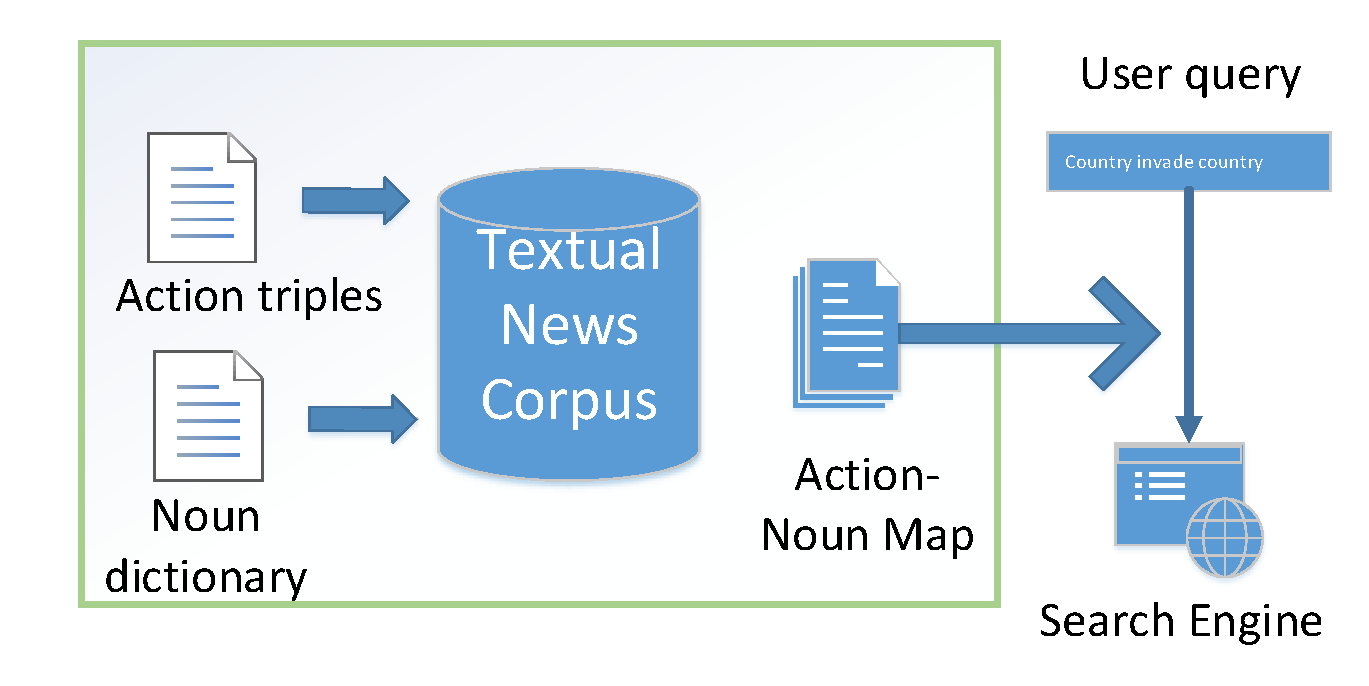
\includegraphics[width=0.95\linewidth]{img/ac1.pdf}
    \caption{workflow}
    \label{fig:workflow}
\end{figure}


The most important component in this project is to
abstract action triples by noun concepts. Here are some definitions we will use throughout
this paper:
\begin{itemize}
\item action concept: A triple consists of subject, predicate and object. Both subject and object are concepts in a predefined set.
    For example, ``country invade country'', ``company buy company'', ``person play instrument'', etc.
\item noun concept: An abstract noun that has multiple instances. 
    In this project we care about those nouns that could summarize an action.  
    For example, ``acquisition'', ``war'', ``performance'' etc.
\item action instance: A triple that is an instantiation of an action concept. Namely the subject and object are instances of the
    subject concept and object concept in action concept. For example, ``Germany invaded France'' would be an instance of ``country 
        invade country'', ``Google bought Deepmind'' would be an instance of ``company buy company''.
\end{itemize}


\section{Calculus}\label{sec:calculus}

In this section, we define a calculus that formally describes the operational semantics
of speculative nondeterminism. We first present the data models of the framework which
is independent of the rest of the calculus. Then we introduce the syntax of the language,
its typing and evaluation rules, and finally we discuss the exit and commit semantics
which are most interesting aspects of the framework.

\subsection{Data Model}\label{sec:datamodel}

Speculative nondeterminism is a programming framework that assumes a centralized
data store that acts as the primary programming environment. The implementation of this store is
not part of the language and therefore independent from the operational semantics of the language.
Here we present the abstract data model of the store that can be instantiated into different
concrete models.
%Typical examples of a data model are tuple space, record space, key-value store, relational model (relations), and logic programs (predicates).
%New data models can also be customized for domain-specific applications and be built on top of existing data models.
%The data model is separated from the speculative choices, which means the data
%model can be changed without affecting the behavior of speculations as long
%as the data model provides the features needed by speculation.

A data model is a 8-tuple
$$\dm=\langle\mkstore,\alltype,\allop,\allstore,\dstype,\vdash,\sqcup,\dtrans\rangle$$
where
\begin{description}
  \item[$\mkstore$] defines an empty data store.
  \item[$\alltype$] is the set of all types available in the data model.
  \item[$\allop$] is the set of all data operations available in the data model.
  \item[$\allstore$] is the set of all possible data stores.
  \item[$\dptype:\allop\to\alltype$] returns the type of an operation.
  \item[$\dstype:\allstore\to 2^\alltype$] returns the set of types of a data store; $\dstype(\mkstore)=\emptyset$.
  \item[$\vdash\subseteq\allstore\times\allop$] is a binary relation
denoted by $d\vdash p$.
It defines when operation $p$ can be executed on the data store $d$.
For example, if the operation $p$ has a precondition, $d\vdash p$ is
true if and only if the condition is true when evaluated on the data store $d$.
  \item[$\sqcup:\allstore\times\allstore\to\allstore$] is a disjoint union function
such that for $d_1\sqcup d_2$, $\dstype(d_1)\cap\dstype(d_2)=\emptyset$.
The disjoint requirement is needed to guarantee safe merge of two stores.
As an example, two key-value stores with overlapped types,
$[a\mapsto 1]$ and $[a\mapsto 2]$, cannot be merged together.
  \item[$\dtrans:\allop\times\allstore\to\allstore$] is the transition function that
defines the effect of data operations on the store. 
It should be guaranteed that $\dstype(\dtrans(p,d))\subseteq\{\dptype(p)\}\cup\dstype(d)$. 
\end{description}

Next we give some examples of concrete data models under the above framework.

\subsubsection*{Data Model for Dining Philosophers Problem}

It's easier to represent the 3 Dining Philosophers Problem with
a customized data model defined below.
A data store is essentially a set of forks on the table. 
This data model assumes just one dining table for brevity.
\begin{align*}
  \mkstore &= \emptyset
\\
  \alltype &= \{ x,y,z \}
\\
  \allop &= \{ -x, -y, -z, +x, +y, +z \}
\\
  \allstore &= 2^\alltype
\\
  \dptype(-w) & =\dptype(+w)=w \text{ where } w\in\alltype
\\
  \dstype(d) &= \alltype
\\
  % \frac{w\in d}{d\vdash -w}, &
  % \hspace*{1ex} \frac{}{d\vdash +w}
  % \text{ where } w\in\alltype
  \vdash &= \{(d,-w):w\in d\}\cup\{(d,+w):w\in\alltype\}
\\
%  d_1\sqcup d_2 & = d_1\cap d_2
%  \\&\text{\em $\sqcup$ merges two data stores by taking the intersection of}
%  \\&\text{\em the two sets, because for example $A$ grabs $x$ and $d_1=$}
%  \\&\text{\em $\{y,z\}$, and $B$ in another galaxy has $d_2=\{x,y,z\}$ and}
%  \\&\text{\em wants to merge with $d_1$, only intersection can correctly}
%  \\&\text{\em merge them.}
  d_1\sqcup d_2 & = d_1\cup d_2
\\
  \dtrans(-w,d) &= d\setminus\{w\},
  \dtrans(+w,d) = d\cup\{w\}
  \text{ where } w\in\alltype
\end{align*}
It is possible to execute $-w$ (to grab the fork $w$) only if $w\in d$ (the fork $w$ is on the table).
To grab a fork $w$ ($-w$) is to remove $w$ from the set $d$, and to put down a fork $w$ ($+w$) is to add $w$ to the set $d$.

\subsubsection*{Tuple Space}

The idea of tuple space comes from Linda \cite{Gelernter85:Linda}, where
a tuple space is a multi-set of tuples that can be accessed concurrently.
Agents can post their data to the tuple space in the form of tuples, and retrieve tuples as data from the tuple space that match a certain pattern.
There are three major operations in the tuple space data model:
\begin{description}
\item[$in$] reads and removes a tuple from a tuple space
\item[$out$] produces a tuple, writing it into a tuple space
\item[$rd$] non-destructively reads a tuple space and gets a copy of a tuple
\end{description}
Formal definitions and operational semantics for
the $in/out/rd$ operations are provided in \cite{Ciancarini95}
which can be easily adapted to this framework.

%\begin{example}[Tuple Space for Trading]
%Data models can not only be customized for domain-specific purposes, as shown in Section \ref{sec:custom3dp},
%but also be built on top of existing data models.
%In this example, two primitive operations for trading, $buy$ and $sell$, are implemented on top of the tuple space data model.
%Only the availability and the type of products being traded are considered, while the prices are ignored for simplicity.
%\setcounter{equation}{0}
%\begin{eqnarray}
%sell(t:\textbf{Product}) :=
%& \mathbf{let} & id=new\_trans\_id() \label{eg:trade:sell:1}\\
%& \mathbf{in}  & out(t,\textbf{sell},id) \label{eg:trade:sell:2} \\
%&     & in(t,\textbf{buy},id) \label{eg:trade:sell:3} \\
%&     & out(t,\textbf{ack},id) \label{eg:trade:sell:4} \\
%buy(t:\textbf{Product}) :=
%& \mathbf{let} & id:\mathbf{integer} \label{eg:trade:buy:1} \\
%& \mathbf{in}  & in(t,\textbf{sell},\mathbf{ref}~id) \label{eg:trade:buy:2} \\
%&     & out(t,\textbf{buy},id) \label{eg:trade:buy:3} \\
%&     & rd(t,\textbf{ack},id) \label{eg:trade:buy:4}
%\end{eqnarray}
%
%As shown above, both $sell$ and $buy$ are presented in pseudo-code form and make use of primitive operations in the tuple space data model such as $in$, $out$ and $rd$.
%
%First we explain the $sell$ operation.
%The function $new\_trans\_id$ allocates a unique transaction number in the form of an integer (line \ref{eg:trade:sell:1}).
%Then a tuple of the product type $t$, the trade type $\textbf{sell}$ and the transaction number $id$ is posted to the tuple space (line \ref{eg:trade:sell:2}).
%Later it waits for a tuple of trade type $\textbf{buy}$ to appear and consumes it by using the $in$ operation (line \ref{eg:trade:sell:3}).
%Finally, it produces an acknowledgement of the transaction being completed (line \ref{eg:trade:sell:4}).
%
%The $buy$ operation is similar to $sell$.
%First the variable $id$ is declared to be an integer (line \ref{eg:trade:buy:1}).
%Next it waits for a tuple of trade type $\textbf{sell}$, which is produced elsewhere in line \ref{eg:trade:sell:2}, and consumes it, filling $id$ with the value of the third element in the tuple (line \ref{eg:trade:buy:2}).
%Then it produces a tuple of trade type $\textbf{buy}$ (line \ref{eg:trade:buy:3}), which will be consumed later in line \ref{eg:trade:sell:3}.
%Finally the acknowledgement is read for confirmation of the completion (line \ref{eg:trade:buy:4}).
%\end{example}

\subsubsection*{Key-value Store}

{\em Key-value store} is a mapping from arbitrary names
(i.e. keys) to arbitrary values.
For example, $[a\mapsto 3, b\mapsto 5]$ is a key-value store
where the key $a$ gets value $3$ and $b$ gets $5$.
The set of types of a key-value store is the set of names in
the store ($\{a,b\}$ in the example). The scope of data operations normally
includes (i) creating a new key-value pair,
(ii) updating an existing key with a new value,
(iii) getting a value according to a key, and
(iv) removing a key and its corresponding value.
Conditional guards can also be combined with these data operations,
e.g., $a>4\Rightarrow b\gets 2$ waits (blocks) until
the condition $a>4$ is true in the store,
and then updates the value of $b$ to $2$.

\subsubsection*{Other Models}
Other more structured data models include relational data and logic programs.
Data operations are insertion and deletion of tuples/predicates. Applications
using these models are also typical.

%{\em Relational model} is a classic and powerful data model. Data is represented by tuples and grouped into relations according to their domain-specific meanings.
%    Conventionally, relations and tuples can be manipulated by using relational algebra or SQL,
%    which is also viable in our framework being the data operation.
%    The types in this relational data model are the relation names,
%    or relation names together with specific ranges of values on a field in condition of data fragmentation.
%
%{\em Logical predicates} can also be used as a data model which can support a knowledge base for inferences.
%The scope of data operations in a logical predicates data model includes monotonically adding rules/facts to the knowledge base, and asking for an evaluation of a predicate.
%


\subsection{Syntax, Typing and Basic Operations}\label{sec:rules}

\begin{figure}
  \centering
  \begin{eqnarray*}
    a & ::= & [e,f] \text{ where } f:\allstore\to\nat \\
    e & ::= & e_1 \oplus e_2 \\ 
      &   | & e_1 . e_2 \\
      &   | & p \text{ where } p\in\allop \\
      &   | & \cm  ~~|~~ \cu  ~~|~~ \epsilon \\
      &     & \\
    U & ::= & \emptyset \\
      &   | & \{G_1,\dots,G_n\} \\
    G & ::= & \langle A,d,s \rangle \text{ where } d\in\allstore, s\in2^{\nat\times\nat} \\
      &   | & G_1 \oplus_k G_2 \text{ where $k\in\nat$ is the identifier of an agent} \\
    A & ::= & [] \\
      &   | & [a_1,\dots,a_m]
  \end{eqnarray*}
  \caption{Syntax and Runtime Data Structures}
  \label{fig:syntax}
\end{figure}

\figref{fig:syntax} first gives the syntax of agent programs 
for a data model.
\begin{description}
\item[$a$] is an agent $[e,f]$ where $e$ is the program and
	$f$ is the exit condition function.
\item[$e_1\oplus e_2$] is the exclusive choice construct.
\item[$e_1.e_2$] is the execution of $e_1$ and $e_2$ in a sequence.
\item[$p\in\allop$] is the data operation defined in the data model.
\item[$\epsilon$] is an empty program indicating the end of a program.
\item[$\cm$ and $\cu$] are primitives for pruning choices, which are described briefly in Section \ref{sec:overview} and formally in Section \ref{sec:commit2}. A well-formed program must have a matching $\cm$ for each choice construct.
However, our semantics framework can both add missing $\cm$'s and ignore redundant $\cm$'s automatically.
\end{description}

\figref{fig:syntax} also defines the runtime data structures 
in the calculus.
\begin{description}
\item[$U$] is a universe, the the top-level structure consisting of a set of galaxies.
The initial state of the universe is $\emptyset$.
\item[$G$] is the galaxy which is either a tree of worlds, or just one world.
A world is a quadruple $\langle A, d, s\rangle$ where $A$
is the list of agents participating in this world,
$d$ is the associated data store,
%$c$ is the set of indices (i.e., numeric identifiers) of committed agents,
and $s$ is the map from agent index to the exit value.
\end{description}

For simplicity we use numeric identifiers for agents throughout this paper.
We also use the following notations for the operations of a list:
(i) $|A|$ is the \emph{length} of the list $A$;
(ii) $A[\cdot]$ means \emph{indexing};
(iii) $A[i\mapsto a]$ replaces the $i$-th element of $A$ with $a$;
(iv) $A+B$ is the \emph{concatenation} of list $A$ and list $B$.

Top of \figref{fig:rules} shows the typing rules of the universe and galaxies.
$\typeof\cdot$ is a set of types which are defined in the given data model.
The set of types of the universe is the union of the sets of types of all the galaxies, 
while the set of types of a galaxy is the union of the sets of types of all the leaf worlds. 
Note that all the types come from the data model.

\begin{figure*}
\begin{minipage}{\textwidth}
  \flushright\fbox{$T=S$} \\
  \begin{minipage}{0.24\textwidth}
    \begin{gather*}
    \frac{}{\typeof U = \bigcup_{G\in U} \typeof G} \\
    \frac{
        {a=[e,f]}\qquad
        {\typeof e = \tau_1}}
      {\typeof a = \tau_1}
    \end{gather*}
  \end{minipage}
  \begin{minipage}{0.24\textwidth}
    \begin{gather*}
    \frac{
        {G = \langle A,d,s\rangle}\quad
        {\dstype(d) = \tau_1}}
    {\typeof{G} = \tau_1} \\
    \frac{
        {\typeof{e_1} = \tau_1}\qquad
        {\typeof{e_2} = \tau_2}}
    {\typeof{e_1\oplus e_2} = \tau_1\cup\tau_2}
    \end{gather*}
  \end{minipage}
  \begin{minipage}{0.24\textwidth}
    \begin{gather*}
    \frac{
        {\typeof{G_1} = \tau_1}\qquad
        {\typeof{G_2} = \tau_2}}
    {\typeof{G_1\oplus G_2} = \tau_1\cup\tau_2} \\
    \frac{
        {\typeof{e_1} = \tau_1}\qquad
        {\typeof{e_2} = \tau_2}}
    {\typeof{e_1.e_2} = \tau_1\cup\tau_2}
    \end{gather*}
  \end{minipage}
  \begin{minipage}{0.12\textwidth}
    \begin{gather*}
    \frac{p \in \allop}{\typeof{p} = \{\dptype(p)\}} \\
    \frac{\quad}{\typeof{\cm} = \emptyset}
    \end{gather*}
  \end{minipage}
  \begin{minipage}{0.12\textwidth}
    \begin{gather*}
    \frac{\quad}{\typeof{\epsilon} = \emptyset} \\
    \frac{\quad}{\typeof{\cu} = \emptyset}
    \end{gather*}
  \end{minipage}
  %%%%
  \flushright\fbox{$U+a\Longrightarrow U'$}
  \[
    \tag{\sc Entrance}\label{rule:birth}
    \frac{}{U + a \Longrightarrow U\cup\{\langle [a],\mkstore,\emptyset,\emptyset\rangle\}}
  \]
  \flushright\fbox{$U\uto U'$}
  \[
    \tag{\sc Merge}\label{rule:merge}
    \frac{
    {\begin{matrix}
              w=\langle A,d,s\rangle \\
              w'=\langle A[i\mapsto[e,f]],d',s'\rangle \\
              s'=\snapshot(s,|e|,i,f(d'))
            \end{matrix}}
            \qquad
    {\begin{matrix}
              G,G'\in U \\
              w\in leaves(G)
            \end{matrix}}
            \qquad
    {\begin{matrix}
              p\in\allop \\
              d\vdash p \\
              d'=\dtrans(p,d)
            \end{matrix}}
            \qquad
    {\begin{matrix}
              {\begin{matrix}
                [p.e,f] = A[i] \\
                \dptype(p)\in\typeof{G'}
              \end{matrix}}
              \qquad
              (1\le i\le |A|)
            \end{matrix}}}
    {U \uto (U\setminus\{G,G'\}) \cup \{\gmerge(replace(G,w,w'),G')\}}
  \]
  \[
    \tag{\sc Alone}\label{rule:alone}
    \frac{
    {\begin{matrix}
              w=\langle A,d,s\rangle \\
              w'=\langle A[i\mapsto[e,f]],d',s'\rangle \\
              s'=\snapshot(s,|e|,i,f(d'))
            \end{matrix}}
            \qquad
    {\begin{matrix}
              G\in U \\
              w\in leaves(G)
            \end{matrix}}
            \qquad
    {\begin{matrix}
              p\in\allop \\
              d\vdash p \\
              d'=\dtrans(p,d)
            \end{matrix}}
            \qquad
    {\begin{matrix}
              {\begin{matrix}
                [p.e,f] = A[i] \\
                \dptype(p)\not\in\typeof{U\setminus\{G\}}
              \end{matrix}}
              \qquad
              (1\le i\le |A|)
            \end{matrix}}}
    {U \uto (U\setminus\{G\}) \cup \{replace(G,w,w')\}}
  \]
%
  \flushright\fbox{$G\gto G'$}\\
  \begin{minipage}{0.59\textwidth}
  \[
    \tag{\sc Fork}\label{rule:fork}
    \frac{
    {[(e_1\oplus e_2).e,f]=A[i]}\qquad
%    {H=A[1..i-1]+A[i+1..|A|]}\quad
%    {c'=shiftc(c,i)}\quad
%    {s'=rs(s,i,|A|)}\quad
    {(1\le i\le |A|)}}
    {\langle A,d,s\rangle \gto
      \langle A[i\mapsto[e_1.e,f]],d,s\rangle \oplus_i
      \langle A[i\mapsto[e_2.e,f]],d,s\rangle}
  \]
  \[
    \tag{\sc Cm}\label{rule:cm}
    \frac{
    {[\cm.e,f]=A[i]}\qquad
%    {\{i+1,\dots,|A|\}\subseteq c}\qquad
    {(1\le i\le |A|)}}
    {G\oplus_i\langle A,d,s\rangle \gto \langle A[i\mapsto[e,f]],d,\snapshot(s,|e|,i,f(d))\rangle}
  \]
  \end{minipage}
  \begin{minipage}{0.4\textwidth}
  \[
    \tag{\sc Swap}\label{rule:swap}
    \frac{}{G_1\oplus_k G_2 \gto G_2\oplus_k G_1}
  \]
  \[
    \tag{\sc Cu}\label{rule:cu}
    \frac{
    {[\cu.e,f]=A[i]}\qquad
    {(1\le i\le |A|)}}
    {\langle A,d,s\rangle\oplus_k G \gto G}
  \]
  \end{minipage}
  \vspace{1ex}
  \[
    \tag{\sc Cm-Auto}\label{rule:cm-auto}
    \frac{
      w\in leaves(G) \qquad
      w=\langle A,d,s\rangle \qquad
      [\epsilon,f]=A[i] \qquad
      i\in cid(G) \qquad
      w'=\langle A[i\mapsto[\cm,f]],d,s\rangle \qquad
      (1\le i\le |A|)
    }
    {G \gto replace(G,w,w')}
  \]
  \[
    \tag{\sc Cm-Skip}\label{rule:cm-skip}
    \frac{
      w\in leaves(G) \qquad
      w=\langle A,d,s\rangle \qquad
      [\cm.e,f]=A[i] \qquad
      i\not\in cid(G) \qquad
      w'=\langle A[i\mapsto[e,f]],d,s\rangle \qquad
      (1\le i\le |A|)
    }
    {G \gto replace(G,w,w')}
  \]
  \vspace{1ex}
  \[
    \tag{\sc Exit}\label{rule:exit}
    \frac{%\displaystyle
    W=leaves(G)
    \qquad \sum_{w\in W} ins(w,i)=0
    \qquad i\not\in cid(G)
    \qquad \left|\bigcup_{w\in W} \{exitval(w,i)\}\right|=1
    \qquad (1\le i\le\max_{w\in W} |w|)}
    {G \gto remove(G,i)}
  \]
  \vspace{1mm}
\end{minipage}
%
\begin{minipage}{0.49\textwidth}\centering
  \begin{gather*}
%    \frac{c'=\{j\in c:j<i\}\cup\{j-1:j\in c \land j>i\}}{shiftc(c,i) = c'} \\
    \frac{s'=\{\langle j,v\rangle\in s:j<i\}\cup\{\langle j-1,v\rangle:\langle j,v\rangle\in s \land j>i\}}{shifts(s,i) = s'}
%    \frac{i\in c}{rc(c,i,m) = shiftc(c,i) \cup \{m\}} \qquad
%    \frac{i\not\in c}{rc(c,i,m) = shiftc(c,i)} \\
%    \frac{\langle i,v\rangle\in s}{rs(s,i,m) = shifts(s,i) \cup \{\langle m,v\rangle\}} ~
%    \frac{i\not\in\{j:\langle j,v\rangle\in s\}}{rs(s,i,m) = shifts(s,i)}
  \end{gather*}
  \begin{gather*}
    \frac{\langle G',r\rangle = rg(G,w,w')}
    {replace(G,w,w') = G'} \\
    \frac{\langle G_1',\textbf{true}\rangle = rg(G_1,w,w')}
    {rg(G_1\oplus_k G_2,w,w') = \langle G_1'\oplus_k G_2,\textbf{true}\rangle} \\
    \frac{\langle G_1',\textbf{false}\rangle = rg(G_1,w,w') \qquad \langle G_2',r\rangle = rg(G_2,w,w')}
    {rg(G_1\oplus_k G_2,w,w') = \langle G_1'\oplus_k G_2',r\rangle} \\
    \frac{}{rg(w,w,w') = \langle w',\textbf{true}\rangle} \qquad
    \frac{w_1\ne w}{rg(w_1,w,w') = \langle w_1,\textbf{false}\rangle}
  \end{gather*}
  \[
  % exitval
    %\tag{\sc EVal}
    \frac{w=\langle A,d,s\rangle \qquad \langle i,v\rangle\in s}
    {exitval(w,i)=v}
  \qquad
    \frac{w=\langle A,d,s\rangle}{|w|=|A|}
  \]
  \[
    \frac{}{\snapshot(s,0,i,v)=s\cup\{\langle i,v\rangle\}}
    \qquad
    \frac{l>0}{\snapshot(s,l,i,v)=s}
  \]
  \begin{gather*}
    \frac{}{|e_1\oplus e_2|=\max(|e_1|,|e_2|)}
    \qquad
    \frac{}{|e_1.e_2|=|e_1|+|e_2|}
  \\
    \frac{p\in\allop}{|p|=1}
    \qquad
    \frac{}{|\epsilon|=0}
    \qquad
    \frac{}{|\cm|=1}
    \qquad
    \frac{}{|\cu|=1}
  \end{gather*}
\end{minipage}
\hspace{5mm}
\begin{minipage}{0.49\textwidth}\centering
  %% galaxy merging functions
  \begin{gather*}
    \frac
      {G=G_1\oplus_k G_2}
      {\gmerge(G,G')=\gmerge(G_1,G')\oplus_k\gmerge(G_2,G')}
  \\
    \frac{}{\gmerge(w,G')=\gpaste(w,G')}
  \end{gather*}
  \begin{gather*}
    \frac
      {w=\langle A,d,s\rangle
      \qquad
      G=G_1\oplus_k G_2}
      {\gpaste(w,G)=\gpaste(w,G_1)\oplus_{k+|w|}\gpaste(w,G_2)}
  \\
    \frac
      {\begin{matrix}
        w=\langle A_0,d_0,s_0\rangle \qquad
        G=\langle A,d,s\rangle \\
        s'=s_0\cup\{\langle i+|w|,v\rangle:\langle i,v\rangle\in s\}
      \end{matrix}}
      {\gpaste(w,G)=\langle A_0+A,d_0\sqcup d,s'\rangle}
  \end{gather*}
  %%
  \[
    \frac{}{cid(G_1\oplus_k G_2)=cid(G_1)\cup cid(G_2)\cup\{k\}} \qquad
    \frac{}{cid(w)=\emptyset}
  \]
  %% Auxiliary Functions for Exit Inference Rules
  \[
  % leaves
    \frac{G=G_1\oplus_k G_2}{leaves(G)=leaves(G_1)\uplus leaves(G_2)}
    \quad
    \frac{}{leaves(w)=\lbb w\rbb}
  \]
  \[
  % #instr
    \frac{w=\langle A,d,s\rangle \qquad [e,f]=A[i] \qquad (1\le i\le |A|)}
    {ins(w,i)=|e|}
  \]
  \begin{gather*}
  % remove
    \frac{G=G_1\oplus_k G_2}
    {remove(G,i)=remove(G_1,i)\oplus_k remove(G_2,i)}
  \\
    \frac{\begin{matrix}
        w=\langle A,d,s\rangle \qquad
%        c'=shiftc(c,i) \qquad
        s'=shifts(s,i)
    \end{matrix}}
    {remove(w,i)=\langle A[1..i-1]+A[i+1..|A|],d,s'\rangle}
  \end{gather*}
\end{minipage}
%
  \caption{Inference Rules}
  \label{fig:rules}
\end{figure*}

\figref{fig:rules} shows all the inference rules used to implement our framework.
The system starts with an empty universe $\emptyset$.
New agents can dynamically enter the system via the $+$ operator.
The entrance of a new agent will create a galaxy with one world by itself,
as shown in \ref{rule:birth}.

When one of the agents is ready to execute some operation $p$
on the data store $d$ (i.e., $d\vdash p$),
rules \ref{rule:merge} and \ref{rule:alone} force the checking of
types involved in that operation.
As mentioned in Section \ref{sec:overview},
worlds are partitioned into galaxies according
to the interests of their associated agents at run-time.
The interest is, in fact, the types here.
\ref{rule:merge} shows the case when the type of the operation $p$
interleaves with the type of galaxy $G'$.
In this case, the current galaxy $G$, has to be merged with the galaxy $G'$,
which contains the required type.
In case there is no need to merge with other galaxies,
i.e., either the type resides in the current galaxy or it is a new type,
the operation $p$ is executed directly,
as shown in rule \ref{rule:alone}.

The main idea of speculative nondeterminism is forking and pruning of choices.
\ref{rule:fork} fires if an agent is reduced to
a choice $(e_1\oplus e_2) .e$,
and it consumes the choice construct in the agent to split the current world of
the agent into two.
When the agent on the lowest level of the galaxy tree structure
executes $\cm$, as shown in rule \ref{rule:cm},
the other side of the choice is pruned.
Similarly, for $\cu$ operations, the current side of the choice is pruned instead,
as shown in rule \ref{rule:cu}.
The key difference between $\cm$ and $\cu$ is that
$\cu$ can be executed in any agent and cause the pruning to takes place immediately,
while $\cm$ can only be executed in the lowest-level agents which are
more localized and less aggressive.
Also $\cm$ is blocking when it is not on the lowest level of the tree,
because non-blocking $\cm$ here potentially consumes more resources 
under the risk of being pruned by the $\cm$ on the lowest level. 
This form of commit semantics is therefore known as \emph{localized commit},
which is described in more details in Section \ref{sec:commit2}.
Finally, the rule \ref{rule:cm-auto} automatically adds a $\cm$ at the end of a program 
in case the program is ill-formed and doesn't have a commit operator that matches
a choice. 
Rule \ref{rule:cm-skip} handles another kind of ill-formed program where
there is more than one $\cm$ for a choice branch. 
In this case, only the first $\cm$ is honored but all subsequent ones are ignored.
We don't need a similar skip rule for $\cu$ because the first $\cu$ in a branch
already prunes the current branch.

Rules without names define the following auxiliary functions.
\begin{description}
\item[$shifts(s,i)$] removes the snapshot of $i$ (i.e. $\langle i,v\rangle$) from $s$ (if applicable) and shifts the indices by 1 of snapshots with index greater than $i$.
A \emph{snapshot} is a pair $\langle i,v\rangle$ where $i$ is an agent's index, and $v$ is the evaluation result of the exit condition function $f_i$ of the agent $i$ at the point of time when agent $i$ finishes execution.
\item[$replace(G,w,w')$] replaces world $w$ in galaxy $G$ with $w'$.
\item[$rg(G,w,w')$] is a helper function for $replace$.
\item[$\gmerge(G,G')$] merges 2 galaxies by pasting $G'$ to the leaves of $G$.
\item[$\gpaste(w,G)$] pastes the copies of $w$ to the leaves of $G$.
\item[$cid(G)$] is the set of all the choice identifiers in $G$.
\end{description}

The transitions on the universe and the galaxies have the following properties. 

\begin{proposition}
The data types of galaxies are disjoint.
\end{proposition}
\begin{proof}[Proof sketch]
For \ref{rule:birth}, $\forall G\in U, \typeof G \cap \typeof\mkstore = \emptyset$.
%
For \ref{rule:merge}, % $\dptype(p)\in\typeof{G'}$, and by the definition of data model,
$\typeof{w'}=\dstype(d')=\dstype(\dtrans(p,d))\subseteq\dstype(d)\cup\{\dptype(p)\}$
$\Rightarrow \typeof{w'}\subseteq\dstype(d)\cup\typeof{G'}=\typeof w\cup\typeof{G'}$. 
\begin{align*}
    & \typeof{\gmerge(replace(G,w,w'),G')} \\
  = & \typeof{replace(G,w,w')}\cup\typeof{G'} \\
  \subseteq & {\textstyle\left(\bigcup_{\tilde w \in leaves(G)\setminus\{w\}} \typeof{\tilde w}\right)} \cup \typeof w\cup\typeof{G'} \\
  = & \typeof G \cup \typeof{G'}
\end{align*}
\begin{align*}
  & \forall G_1\in U, \typeof{G_1}\cap\typeof G=\emptyset, \typeof{G_1}\cap\typeof{G'}=\emptyset  \\
  \Rightarrow & \typeof{G_1} \cap (\typeof{G}\cup\typeof{G'}) = \emptyset \\
  \Rightarrow & \typeof{G_1} \cap \typeof{\gmerge(replace(G,w,w'),G')} = \emptyset
\end{align*}
The same applies to \ref{rule:alone}. 

For rules \ref{rule:fork}, \ref{rule:swap}, \ref{rule:cm}, and \ref{rule:exit}, 
the data stores do not change. 
%
For \ref{rule:cu}, data store $d$ is removed. 
Let $G_0=\langle A,d,c,s\rangle\oplus G$.
\begin{align*}
  \forall G_1\in U, \typeof{G_1}\cap\typeof{G_0}=\emptyset
  & \Rightarrow \forall t\in\typeof{G_1}, t\not\in\typeof{G_0} \\
  \typeof{G_0}=\dstype(d)\cup\typeof G
%  & \Rightarrow t\not\in\dstype(d)\text{ and }t\not\in\typeof G \\
  & \Rightarrow t\not\in\typeof G \\
  & \Rightarrow \typeof{G_1}\cap\typeof G=\emptyset
\end{align*}
\end{proof}

\begin{proposition}
An agent lives in one and only one galaxy.
\end{proposition}
\begin{proof}[Proof sketch]
For \ref{rule:birth}, $a$ by itself is one galaxy.

For \ref{rule:merge}, assume $a$ lives in only one galaxy in $U$. 
If $a$ lives in $G$ or $G'$, it still lives in $\gmerge(replace(G,w,w'),G')$.
Otherwise, it lives in $U\setminus\{G,G'\}$.
The same applies to \ref{rule:alone}. 

All the other rules do not move agents between galaxies. 
\end{proof}

\begin{proposition}
Given the empty universe and $n$ agents each with at most $k$ choices, 
if $\bigcap_{i=1}^n \typeof{a_i} = \emptyset$ then the number of simultaneous worlds is at most $kn$.
\end{proposition}
\begin{proof}[Proof sketch]
$\bigcap_{i=1}^n \typeof{a_i} = \emptyset \Rightarrow \forall 1\le i<j\le n, \typeof{a_i}\cap\typeof{a_j}=\emptyset.$
So all the agents live in their own galaxies and will not merge together. 
Then there will be $n$ galaxies. 
For $k$ choices there will be at most $k$ worlds corresponding to them. 
Hence, the number of simultaneous worlds is at most $kn$.
\end{proof}


\subsection{Exit Semantics}\label{sec:exit}

Rule \ref{rule:exit} in Figure \ref{fig:rules} shows the exit semantics.
\begin{description}
\item[$leaves(G)$] returns a multi-set of the leaf worlds in the tree structure of a galaxy $G$.
\item[$ins(w,i)$] counts the number of instructions left (to be executed) in the $i$-th agent program in world $w$.
\item[$exitval(w,i)$] retrieves the evaluation result of the exit condition function of the $i$-th agent when it stops in world $w$.
\item[$|w|$] is the number of agents in world $w$.
\item[$remove(G,i)$] removes the $i$-th agents from all the worlds in galaxy $G$.
\end{description}

Basically \ref{rule:exit} lists all the worlds in the galaxy, counts the number of instructions to ensure the $i$-th agent has completed (i.e. reduced to the empty program $\epsilon$) in all the worlds, and applies the exit condition function to ensure the evaluated results are the same across all the worlds.
When all these conditions are satisfied, the $i$-th agent can exit from the galaxy.

In general, if the states are \emph{consistent} across all the worlds at
the point when the agent completes, the agent can exit immediately.
However, the agent may complete at different wall clock times in different worlds.
In order to capture the values of the exit condition function $f$ applied to different worlds,
$f$ has to be evaluated immediately when the agent becomes $\epsilon$ in a world,
and the evaluated results, namely \emph{snapshots}, are stored as meta data of that world.
The meta data  persists even if this world evolves into multiple worlds later.

Formally, for a world $\langle A,d,s\rangle$,
the snapshots are stored in the map $s$.
At the bottom of Figure \ref{fig:rules},
the function $\snapshot(s,l,i,v)$ is defined as an auxiliary function for taking snapshots,
where $s$ is the current snapshot store of the world,
$l$ is the remaining length of the $i$-th program,
and $v$ is evaluated result of $f$ on the current world.

The exit condition function $f:\allstore\to\nat$
takes a data store as input,
and returns an integer as the evaluated result.
The data store is just the one associated with the current world.
According to the data store,
the exit condition function is expected to produce an integer which can be
a 0/1 indicator, a heuristic value, or an encoding of more complicated
mathematical objects. For example, in the simplest case, $f(d)\equiv 1$
allows the agent to exit without any condition as long as it completes execution
of all the operations in the program.
The ability to return an integer as the snapshot provides the flexibility and
enables complex exiting logic to be embedded in this exit condition function.

The exit semantics gives rise to the following properties.

\begin{proposition}[Causality] If agent $a$ exits in a galaxy $G$,
then the snapshot of this exit must persist in subsequent evolution of $G$.
\end{proposition}
\begin{proof}[Proof sketch]
It follows immediately from rule \ref{rule:fork} and rule \ref{rule:exit}. 
\end{proof}

\begin{proposition}
\label{prop-exit}
We define a world to be empty if there's no program associated with it.
For any given galaxy $G$, either all its world are empty or none of the worlds are
empty.
\end{proposition}
\begin{proof}[Proof sketch]
First, by rule \ref{rule:birth} and \ref{rule:fork}, an agent in galaxy $G$ lives 
in all the worlds of $G$. 
Then by rule \ref{rule:exit}, an agent either entirely leaves $G$ from all the worlds, 
or stays as is. 
So an agent cannot partly lives in some of the worlds. 
Hence, for galaxy $G$, either all its world are empty or none of the worlds are
empty.
\end{proof}
% \begin{proof}[Proof sketch]
% Suppose there is the case that some of the worlds are empty while some others are not. 
% 
% Let $|w| = |\langle A,d,s\rangle| = |A|$ be the number of programs in world $w$. 
% $w$ is \emph{empty} if and only if $|w| = 0$. 
% Make induction on $|w|$. 
% 
% For \ref{rule:birth}, $|\langle[a],\mkstore,\emptyset,\emptyset\rangle|=1$. 
% For \ref{rule:merge}, $|w|=|w'|,$ and by Lemma \ref{lemma:merge2}, 
% $$\forall w_1,w_2\in\gmerge(replace(G,w,w'),G'), |w_1|=|w_2|.$$
% $|w|=|w'|$ also indicates for \ref{rule:alone},
% $$\forall w_1,w_2\in replace(G,w,w'), |w_1|=|w_2|.$$
% 
% For \ref{rule:fork}, \ref{rule:swap}, \ref{rule:cm} and \ref{rule:cu}, 
% $|w|$ is not changed for any $w$. 
% 
% For \ref{rule:exit}, by Lemma \ref{lemma:remove}, 
% $$\forall w_1,w_2\in remove(G,i), |w_1|=|w_2|.$$
% 
% So for any galaxy $G$, all the worlds in $G$ have the same number of programs. 
% Contradiction.
% \end{proof}

\begin{theorem}
Given $n$ agents, and if all agents have exit from the system, 
then there are at most $n$ galaxies left, and each of the galaxies is a world. 
\end{theorem}
\begin{proof}[Proof sketch]
On one hand, the extreme case is all the $n$ agents have absolutely different interests such that 
they do not interleave with each other and live in their own galaxies. In this case 
it is trivial to conclude there will be at most $n$ galaxies left. 

On the other hand, speculation is required to be \emph{exclusive} choice which means 
there will at least be one world existing.
Also the choice construct is required to be paired with commits, and 
extra commits are ignored according to rule \ref{rule:cm-skip}. 
After all the agents exit, they must have finished executing all the operations.
Therefore in the end the galaxy is a world. 
\end{proof}


\subsection{Commit Semantics}\label{sec:commit2}

\begin{figure}
  \centering
  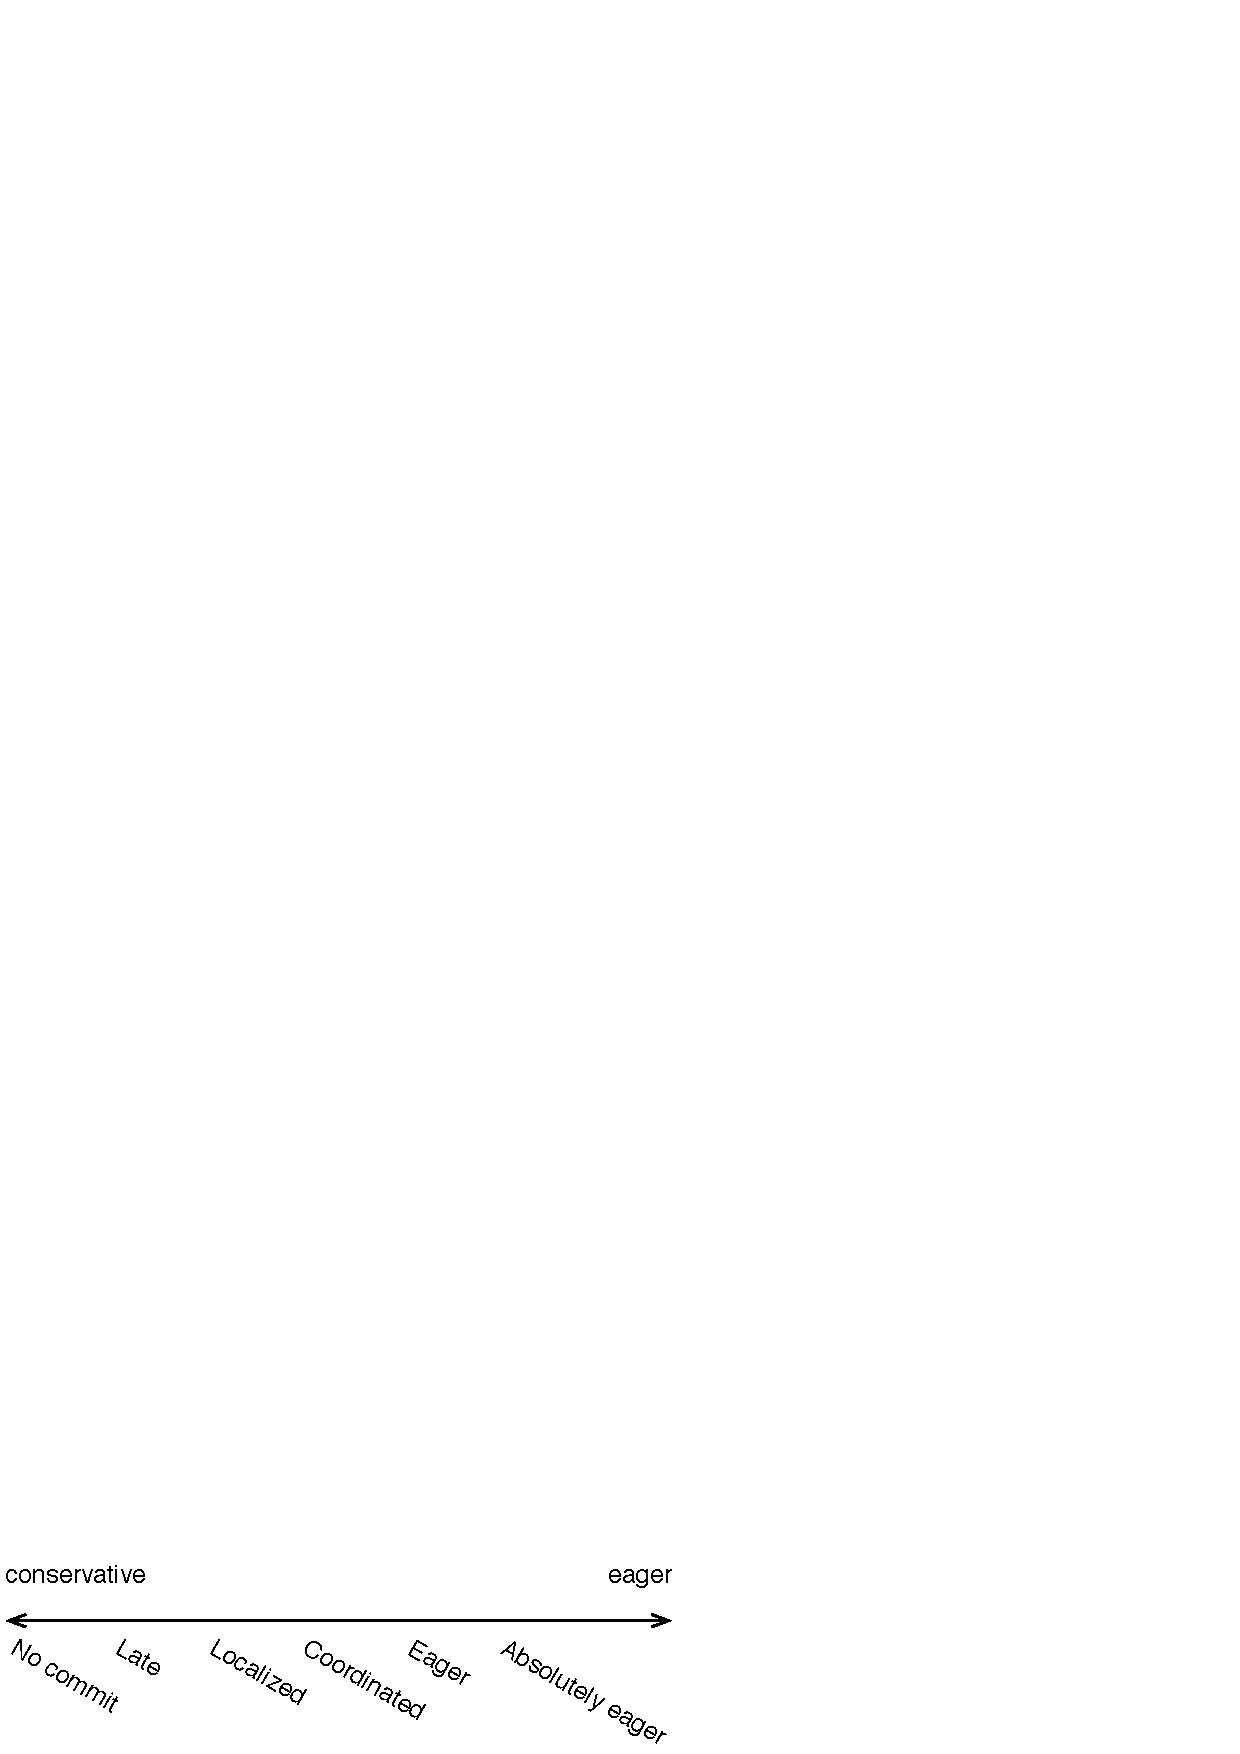
\includegraphics[width=0.4\textwidth]{commit-spectrum}
  \caption{Approximate Spectrum of Commit Semantics}
  \label{fig:commit-spectrum}
\end{figure}

Commits are used to control the run-time behavior,
mostly to prune choices for the purpose of performance.
The commit semantics described in Section \ref{sec:rules} and
in \figref{fig:rules} is called {\em localized commit} as it restricts
the scope of pruning to be of height 1 only.  $\cm$ by agent $X$ cannot
prune until the direct parent of the committed world is $\oplus_X$.
$\cu$ kills the current world immediately without coordination with other worlds.

Besides localized commit, in this section, we identify a number of other possible commit
semantics. They differ in their eagerness to prune the worlds.
They are ordered roughly from the most eager to the most conservative:
{\em absolutely eager commit}, {\em eager commit}, {\em coordinated commit}, {\em late commit}
and {\em no commit} (See \figref{fig:commit-spectrum}).
%The semantics of commits may be different and there are also 4 other commit semantics in order to support different types of pruning.
%They are the absolutely eager commit, the eager commit, the late commit, and the coordinated commit.
%Different commit semantics vary between the range of being conservative and eager, which is depicted in Figure \ref{fig:commit-spectrum}, where the ``none'' means no commit at all (i.e. to generate all the combinatorial choices).
%
We compare and contrast the behavior of these commit semantics
using the dining philosopher example and reason why localized commit
is the chosen semantics in the calculus.
Here we are only concerned with the shape of the tree structures
after different commits and ignore the details in the world (leaf nodes).
The initial structure is in \figref{fig:cmcmp:init},
and let's see the effect of $B$ committing in $w_1$.
\begin{description}
  \item[Absolutely eager commit] is the most aggressive form of commit and
as soon as one agent commits in one of the worlds,
it kills {\em all} the other worlds. As illustrated in
\figref{fig:cmcmp:abs}, system immediately prunes the whole sub-tree.

  \item[Eager commit] is less aggressive and kills the branch on the right
immediately once there is a commit in the branch on the left.
\footnote{Note that the terms ``left branch'' and ``right branch'' in this
discussion are symbolic and can be used interchangeably.}
This can be seen in \figref{fig:cmcmp:eager}.

  \item[Late commit] kills the branch on the right only if all occurrences
(not necessarily in the same scope) of the (syntactically) left branch commit.
In the example, it requires $B$ commits not only in $w_1$,
but also in $w_2$, $w_5$ and $w_7$ and prunes all the right-hand side of
$\oplus_B$ (\figref{fig:cmcmp:late}).

  \item[Coordinated commit] proposed in our previous work \cite{JaffarYZ07}
is a compromise between the eager commit and the late commit, which does not
kill the alternative choice until $\cm$ of this choice has been reached in
\emph{all} worlds in the {\em scope} of the choice construct.
In our example, this requires $B$ commits in both $w_1$ and $w_2$ and prunes
in the same way as the eager commit (\figref{fig:cmcmp:coord}).
%(i.e. the conjunctive view $\mathcal{CV}$); $\cu$ also uses $\mathcal{CV}$

  \item[No commit] is the naive behavior of ignoring all the $\cm$ or $\cu$
in the program. The net effect of this is that the universe can only grow and
doesn't shrink by itself even if all agents have reached completion and exit in all worlds.
The advantage of this is that if there is a solution for all the agents, this semantics
will find it, the disadvantage is the computation space is exponential.
If no-commit semantics is used, in this example, the shape of the tree
remains the same as the initial structure till the end.
To reclaim system resources, system could employ a global collapse rule below
to reduce a galaxy that has no more agents to a single world. And due to the
exit semantics and Property \ref{prop-exit},
any world in this galaxy can become the new galaxy.
\[
    \tag{\sc Collapse}\label{rule:collapse}
    \frac
    {\langle [], d, s \rangle \in leaves(G) }
    {G \gto \langle [], d, s \rangle}
\]


\item[Localized commit] cannot prune until $C$ commits in $w_1$ as well, because the reason for $B$ to commit in $w_1$ may be that $C$ lives in $w_1$. When $C$ commits in $w_1$, the tree structure becomes an intermediate state as shown in the left-hand side of Figure \ref{fig:cmcmp:local}. Then the pending commit from $B$ is executed and prunes in the same way as the absolutely eager commit eventually (right-hand side of Figure \ref{fig:cmcmp:local}). It is more conservative but can kill as many as the absolutely eager commit.
\end{description}

\begin{figure*}
\centering\small
\subfigure[Initial galaxy structure]{\label{fig:cmcmp:init}
\begin{minipage}{0.325\textwidth}
\Tree[.$\oplus_A$
    [.$\oplus_{B_1}$
        [.$\oplus_{C_1}$
            $w_1$
            $w_2$
        ]
        [.$\oplus_{C_2}$
            $w_3$
            $w_4$
        ]
    ]
    [.$\oplus_{C_3}$
        [.$\oplus_{B_2}$
            $w_5$
            $w_6$
        ]
        [.$\oplus_{B_3}$
            $w_7$
            $w_8$
        ]
    ]
]
\end{minipage}
}
\subfigure[Absolutely eager commit]{\label{fig:cmcmp:abs}
\begin{minipage}{0.195\textwidth}
\Tree[.$\oplus_A$
    $w_1$
    [.$\oplus_{C_3}$
        [.$\oplus_{B_2}$
            $w_5$
            $w_6$
        ]
        [.$\oplus_{B_3}$
            $w_7$
            $w_8$
        ]
    ]
]
\end{minipage}
}
\subfigure[Eager commit]{\label{fig:cmcmp:eager}
\begin{minipage}{0.225\textwidth}
\Tree[.$\oplus_A$
    [.$\oplus_{C_1}$
        $w_1$
        $w_2$
    ]
    [.$\oplus_{C_3}$
        [.$\oplus_{B_2}$
            $w_5$
            $w_6$
        ]
        [.$\oplus_{B_3}$
            $w_7$
            $w_8$
        ]
    ]
]
\end{minipage}
}
\subfigure[Late commit]{\label{fig:cmcmp:late}
\begin{minipage}{0.21\textwidth}
\centering
\begin{tabular}{c}
\\
\Tree[.$\oplus_A$
    [.$\oplus_{C_1}$
        $w_1$
        $w_2$
    ]
    [.$\oplus_{C_3}$
        $w_5$
        $w_7$
    ]
] \\ \\ \\
\end{tabular}
\end{minipage}
}
\subfigure[Coordinated commit]{\label{fig:cmcmp:coord}
\begin{minipage}{0.25\textwidth}
\Tree[.$\oplus_A$
    [.$\oplus_{C_1}$
        $w_1$
        $w_2$
    ]
    [.$\oplus_{C_3}$
        [.$\oplus_{B_2}$
            $w_5$
            $w_6$
        ]
        [.$\oplus_{B_3}$
            $w_7$
            $w_8$
        ]
    ]
]
\end{minipage}
}
\subfigure[Localized commit]{\label{fig:cmcmp:local}
\begin{tabular}{cccc}
$\quad$
&
\begin{minipage}{0.27\textwidth}
\Tree[.$\oplus_A$
    [.$\oplus_{B_1}$
        $w_1$
        [.$\oplus_{C_2}$
            $w_3$
            $w_4$
        ]
    ]
    [.$\oplus_{C_3}$
        [.$\oplus_{B_2}$
            $w_5$
            $w_6$
        ]
        [.$\oplus_{B_3}$
            $w_7$
            $w_8$
        ]
    ]
]
\end{minipage}
&
$\Rightarrow$
&
\begin{minipage}{0.18\textwidth}
\Tree[.$\oplus_A$
    $w_1$
    [.$\oplus_{C_3}$
        [.$\oplus_{B_2}$
            $w_5$
            $w_6$
        ]
        [.$\oplus_{B_3}$
            $w_7$
            $w_8$
        ]
    ]
]
\end{minipage}
\end{tabular}
}
\caption{Illustration of Different Commit Semantics}
\label{fig:cmcmp}
\end{figure*}

In general, the coordinated commit proposed previously \cite{JaffarYZ07}
has two disadvantages:
\begin{enumerate}
  \item The most attractive feature of coordinated commit is the ability to
  prune not only leaf worlds but also subtrees of worlds,
  but the condition for this to happen requires $\cm$ of this choice to be reached
  in the scope of the choice construct, in all worlds.
  However, it is costly to do so as it needs to maintain information
	of the {\em conjunctive views} of many data stores. \footnote{Conjunctive view
of a set of stores $D$ is the common data in $D$.}
  \item As shown in the following example, it may prune the only world
	where all agents can be satisfied.
\end{enumerate}

\begin{figure}[th]
  \centering
  \small\Tree[.$\oplus_X$
          [.$\oplus_Y$
            {$X:+\alpha.\cm_1$\\$Y:\underline{-\beta}.\cm$\\ \\ $(X_l Y_l)$}
            {$X:+\alpha.\cm_2$\\$Y:\underline{-\gamma}.\cm$\\ \\ $(X_l Y_r)$}
          ]
          [.$\oplus_Y$
            {$X:+\beta.\cm_3$\\$Y:-\beta.\cm_5$\\ \\$(X_r Y_l)$}
            {$X:+\beta.\cm_4$\\$Y:\underline{-\gamma}.\cm$\\ \\ $(X_r Y_r)$}
          ]
        ]
  \caption{Runtime Galaxy Structure for Programs $X$ and $Y$}
  \label{fig:commit-example}
\end{figure}


Let's consider the following simple program to understand why the localized commit is better
than the other pruning-based commit semantics and chosen as the default semantics in
our calculus. Suppose there are two agent programs $X$ and $Y$:
\begin{eqnarray*}
  X: & +\alpha.\cm\oplus +\beta.\cm \\
  Y: & -\beta.\cm\oplus -\gamma.\cm
\end{eqnarray*}

A possible runtime galaxy structure is shown in Figure \ref{fig:commit-example}
where $\oplus_X$ starts before $\oplus_Y$.
$X$ and $Y$ are subscripted with $l$ and $r$ which means
the left-hand side and the right-hand side respectively.
The underlined parts are blocked while all other operations can be executed successfully.
Subscripts of $\cm$ indicate the execution order of the commit actions.
Consider the effects of different commit semantics in Figure \ref{fig:commit-example}.

Absolutely eager commit prunes all the three worlds $X_l Y_r$, $X_r Y_l$ and $X_r Y_r$
when $\cm_1$ is executed.
Eager commit prunes both $X_r Y_l$ and $X_r Y_r$ when $\cm_1$ is executed.
Late commit waits until both $\cm_1$ and $\cm_2$ are executed and then prunes both
$X_r Y_l$ and $X_r Y_r$.
Coordinated commit is the same as late commit in this example.
Localized commit prevents $\cm_1$ and $\cm_2$ from pruning worlds
because the commits are issued by $X$ while the parent of $X_l Y_l$ and $X_l Y_r$ is $Y$;
only until $\cm_5$ is executed in world $X_r Y_l$ and
prunes $X_r Y_r$, the pending commit $\cm_3$ prunes both
$X_l Y_l$ and $X_l Y_r$.

\section{Analysis}
\label{sec:analysis}

% Analyze the main algo: time complexity, space complexity.
% Some properties to consider:
%
% \begin{itemize}
% \item give a bound on the total number of items suppressed;
% \item give a bound on the deviation in distribution from the original data;
% \item give a bound on the number of association rules that we eliminate;
% \item and what else??
% \end{itemize}

In this section, we show several interesting properties of our algorithm.
%in order to provide an all-aspect analysis of the problem and our algorithm.

%\begin{theorem}
%  The Optimal Suppression Problem in Definition \ref{def:osp} is NP-hard.
%\end{theorem}
%% TODO prove the whole problem hierarchy
%\begin{proof}
%  TODO
%\end{proof}

\begin{lemma}
\label{lemma:rule}
  If the inference $\mathcal{A}(q,a)$ is safe,
  then  $\mathcal{A}(q,a, b_1,b_2,\dots,b_n)$ is safe for any sequence of $\{b_i\}$.
\end{lemma}
\begin{proof}
  \begin{align*}
    \text{$q\rightarrow a$ is safe}
    \Rightarrow
    &\, \frac{\csize(q\cup\{a\})}{\csize(q)} \le \rho \\
    \Rightarrow
    &\, \csize(q\cup\{a\}) \le \rho\cdot\csize(q)
  \end{align*}
  \begin{align*}
    &\, (q\cup\{a\}) \subset (q\cup\{a, b_1,b_2,\dots,b_n\}) \\
    \Rightarrow
    &\,  \csize(q\cup\{a, b_1,b_2,\dots,b_n\}) \leq \csize(q\cup\{a\}) \le \rho\cdot\csize(q) \\
    \Rightarrow
    &\, \frac{\csize(q\cup\{a, b_1,b_2,\dots,b_n\}}{\csize(q)} \le \rho \\
    \Rightarrow
    &\, \text{$q\rightarrow a, b_1,b_2,\dots,b_n$ is safe}
  \end{align*}
\end{proof}

Lemma \ref{lemma:rule} shows that we do not have to consider rules with consequent of length 2 or longer.

\begin{lemma}%[Correctness of partitioning]
\label{CorrectnessOfPartitioning}
  If $q$ is safe in both $T_1$ and $T_2$, then $q$ is safe in $T = T_1 \cup T_2$.
\end{lemma}
\begin{proof}
For any item $a$,
  \begin{align*}
   q~\text{is safe in}~T_1 &\Rightarrow \csize_{T_1}(q\cup\{a\}) \le \rho\cdot\csize_{T_1}(q) \\
   q~\text{is safe in}~T_2 &\Rightarrow \csize_{T_2}(q\cup\{a\}) \le \rho\cdot\csize_{T_2}(q)
  \end{align*}
  So \begin{align*}
   \csize_{T_1}(q\cup\{a\}) + \csize_{T_2}(q\cup\{a\}) &\le \rho\cdot\csize_{T_1}(q) + \rho\cdot\csize_{T_2}(q)
  \end{align*}
  And \begin{align*}
    \csize_T(q\cup\{a\}) &= \csize_{T_1}(q\cup\{a\}) + \csize_{T_2}(q\cup\{a\}) \\
    \csize_T(q) &= \csize_{T_1}(q) + \csize_{T_2}(q)
  \end{align*}
  So $$ \frac{\csize_T(q\cup\{a\})}{\csize_T(q)} \le \rho~\Rightarrow q~\text{is safe in}~T .$$
\end{proof}

\begin{theorem}
\label{CorrectnessOfPartialSuppressor}
  \PartialSuppressor always terminates with a correct solution.
\end{theorem}
\begin{proof}
We first prove that if the algorithm terminates, the suppressed table is safe.
Note that the algorithm can only terminates on Line \ref{line:partial-suppressor-break}
  in Algorithm \ref{algo:partialsuppressor}.
So the value of $u$ on Line \ref{line:partial-suppressor-if-u} must always be \FALSE
  until the record cursor $i$ exceeds the table size $|T|$.
That means both \HandleShortRecords and \HandleLongRecord always return
  a pair with \FALSE as the first element during some pass of scanning of the whole table.
For \HandleShortRecords, returning \FALSE on Line \ref{line:handle-short-return-false}
  in Algorithm \ref{algo:handleshort} indicates there is no unsafe \qid in the buffer $B$.
For \HandleLongRecord, returning \FALSE on Line \ref{line:handle-long-return}
  in Algorithm \ref{algo:handlelong} indicates all the \qids generated by \Enum are safe.
So these return values of the two functions indicate there is no unsafe \qid in the table.
Hence, the suppressed table is safe.

Then we prove that \PartialSuppressor always terminates by measuring the
  number of items left (denoted $l$) in the table after each step of suppression.
Initially, $l=l_0=\sum_{i=1}^{|T|} |T[i]|\le |D| |T|$.
We state that for every invocation of \SanitizeBuffer, Line \ref{line:sanitize-suppress}
  in Algorithm \ref{algo:sanitize} is always executed at least once.
So the value $l$ strictly decreases when \SanitizeBuffer is invoked.
And before the table becomes safe, \SanitizeBuffer will be invoked for
  every iteration of the loop in Algorithm \ref{algo:partialsuppressor}.
So $l$ strictly decreases for each loop iteration in \PartialSuppressor.
Because $l$ starts from a finite number which is at most $l_0=\sum_{i=1}^{|T|} |T[i]|$,
  \PartialSuppressor must terminate.
Otherwise there will be an infinite descending chain of all the $l$ values.

Now we prove that Line \ref{line:sanitize-suppress} in Algorithm \ref{algo:sanitize}
  is always executed once \SanitizeBuffer is invoked.
Whenever \SanitizeBuffer is invoked, it is guaranteed that there exists
  an unsafe \qid $q\in B$ (see Line \ref{line:handle-short-if-contains-unsafe} in Algorithm \ref{algo:handleshort}
  and Line \ref{line:handle-long-if-contains-unsafe} in Algorithm \ref{algo:handlelong}).
$q$ is unsafe so that there always exists an item $e\in\linked(q)$ such that $P(e|q)>\rho$,
  i.e. \[ \frac{\csize(q\cup\{e\})}{\csize(q)}>\rho \Rightarrow \csize(q\cup\{e\})-\rho\cdot\csize(q)>0 .\]
For $k$ on Line \ref{line:sanitize-k1} in Algorithm \ref{algo:sanitize},
  \[ k = |X|-\lfloor\rho\cdot\csize(q)\rfloor = \csize(q\cup\{e\})-\lfloor\rho\cdot\csize(q)\rfloor \ge 1 .\]
For $k$ on Line \ref{line:sanitize-k2} in Algorithm \ref{algo:sanitize},
  it is guaranteed that the number of deletions is at least 1
  because the rule $q\rightarrow e$ is unsafe and there must be some deletions to make it safe.
So $k\ge 1$ on Line \ref{line:sanitize-while-k} for the first time.
Thus the condition is satisfied and Line \ref{line:sanitize-suppress} is executed.
\end{proof}

\begin{corollary}
The divide-and-conquer optimization \SplitData is correct.
\end{corollary}
\begin{proof}
It follows directly from Lemma \ref{CorrectnessOfPartitioning} and
Theorem \ref{CorrectnessOfPartialSuppressor}.
\end{proof}

%\begin{theorem}
%Let %$M = |T|$ be the size of table $T$,
%$l$ be the average record length,
%$c = r_r r_d$ where $r_r$ is the regression rate and $r_d$ is the qid duplicate rate.
%The average time complexity of \PartialSuppressor is
%\[ O(c \cdot 2^l |T|^2 l (\bmax (1-\rho) + l)). \]
%\end{theorem}
%\begin{proof}
%{\small\begin{verbatim}
%  general idea:
%  l1 <- estimate the number of iterations
%    for the loop in algorithm 1 -- assume
%    there is a parameter: regression ratio
%  may have to assume the data in some distribution
%    (e.g. power-law) -- related to Figure 1
%    count the number of invocations of HandleShort
%      --> b_max
%    count the number of invocations of HandleLong
%  l2 <- estimate the number of iterations
%    for the loop in algorithm 3
%  l1+l2 -> the number of invocation of SanitizeBuffer
%  estimate complexity of SanitizeBuffer
%  estimate complexity of line 7 to 13 in algorithm 3
%    (related to distribution in Figure 2)
%  estimate the complexity of UpdateBuffer
%\end{verbatim}}]

%Let $n_1$ be the number of short records,
%$n_2$ be the number of long records,
%$p(i)$ be the probability of a record being length $i$,
%$l_m$ be the maximum record length,
%$t=1-\rho$.
%
%Let $v_1$ be the number of invocations of \HandleShortRecords.
%In the process of generating qids and filling them into the qid buffer $B$,
%duplicates cannot be counted.
%If duplicates are allowed, the number of qids generated by a record is
%just $r=\sum_{i=1}^{\lmin-1} p(i)\cdot\#qid(i)$ where
%$\#qid(i)$ is the expected number of qids generated by a record of length $i$.
%Then $\bmax/r$ records are used to fill the buffer (duplicates allowed).
%So roughly $v_1=\frac{n_1\cdot r}{\bmax r_d}$ times to consider all distinct qids
%in short records, for a single pass.
%
%For \HandleLongRecord, the number of invocations is $v_2=n_2$ if
%we do not take multiple passes of table scanning (i.e., the loop in algorithm 1) into consideration.
%Assume the loop in \HandleLongRecord is iterated for $v_3$ times, then \SanitizeBuffer is
%roughly invoked for $v_1 + v_2 v_3$ times.
%
%There are 4 major parts in the computation. We will consider them one by one.
%
%The first part is Line 4 to 7 in Algorithm 2, since the buffer capacity is $\bmax$,
%the maximum number of iterations here is roughly $\bmax r_d$.
%\HandleShortRecords will be invoked for $v_1$ times, so
%the total time cost by this part of computation is roughly $v_1 \bmax r_d$.
%
%The second part is \UpdateBuffer in Algorithm 2. For the invocation
%$\UpdateBuffer(B, T, i, j, K, L)$, the purpose is to update $K$ and $L$
%by considering qids in records $T[i..j]$ which are also in $B$.
%So a single call invocation of \UpdateBuffer costs roughly $(j-i+1)|B|$.
%Hence, the total time cost by this part of computation is roughly
%$v_1 (|T| - \frac{\bmax}{r}) \bmax$.
%
%The third part is Line 7 to 13 in Algorithm 3. Note that in reality
%the computation from Line 10 to 12 can be done at the same time when
%calculating Line 8. And in the worst case, the total time cost by calculating
%these intersections is $\dnum l_m |T|$. And the total time cost by
%this part of computation is $v_2 v_3 \dnum l_m |T|$.

%The fourth part is all the invocations of \SanitizeBuffer.
%For a single invocation of \SanitizeBuffer, there are two sub-parts to consider.
%The first sub-part is the intersection calculation on Line 5 in Algorithm 4,
%which costs roughly $l |T|$.
%The second sub-part is the computation from Line 14 to 25 in Algorithm 4,
%which costs roughly $k |B|$, where $k$ is determined on Line $9$.
%In the worst case, $k= t |T|$.
%So for a single invocation of \SanitizeBuffer, the time cost is roughly
%$|B| r_r l (|T| L + t |T| |B|)$ where $|B|$ is the size of the buffer.
%Because \SanitizeBuffer is invoked $v_1$ times in \HandleShortRecords,
%with buffer size $\bmax$, and $v_2 v_3$ times in \HandleLongRecord,
%with buffer size $\dnum$,
%the total time cost by this part of computation is roughly
%$v_1 \bmax r_r l (l |T| + t |T| \bmax) + v_2 v_3 \dnum r_r l (l |T| + t |T| \dnum)$.
%
%Summing up these four parts we can get the following time cost.
%\begin{align*}
%  n_1 r
%+ \frac{n_1 (r |T| - \bmax)}{r_d}
%+ \frac{n_1 |T| r l r_r (\bmax t + l)}{r_d} \\
%+ l_m |T| n_2 \dnum v_3
%+ l |T| n_2 \dnum v_3 r_r (l + \dnum t)
%\end{align*}
%By eliminating non-denominating terms, we get the order of \[ O(c \cdot 2^l |T|^2 l (\bmax (1-\rho) + l) ) .\]
%\end{proof}
%
%For a given dataset, the expected time complexity is actually quadratic to the size of the table.

%\begin{theorem}
%  The space complexity of \PartialSuppressor on table $T$ is \[ O(\sum_{i=1}^{|T|} |T[i]| + \bmax) .\]
%\end{theorem}
%\begin{proof}
%Let $N = \sum_{i=1}^{|T|} |T[i]|$, then $N$ is the sum of the numbers
%of all item occurrences.
%This term is easy to explain since the algorithm has to store
%the original table $T$.
%So we only need to consider local data structures
%created in \PartialSuppressor
%and related functions for the term $O(\bmax)$.
%
%For \PartialSuppressor, the most significant memory cost is from the \qid buffer of size $\bmax$.
%For \HandleShortRecords, there is only $O(1)$ extra memory space for loop variables like $j$.
%For \HandleLongRecord, there is also $O(1)$ extra memory cost.
%For \SanitizeBuffer, except for the $O(1)$ memory space for local variables, it also involves
%  the storage of $\linked(\cdot)$ and $\csize(\cdot)$.
%Because all the \qids updated are from the buffer $B$, the total number of \qids being active at any time
%  is no greater than the capacity of the buffer, i.e. $\bmax$.
%In order to keep the information of $\linked(\cdot)$ and $\csize(\cdot)$,
%  there will be $O(\bmax)$ extra memory space used.
%\end{proof}

%\begin{theorem}
%  The algorithm suppresses at most $O(xxx)$ item occurrences on average.
%\end{theorem}
%\begin{proof}
%  TODO
%\end{proof}
%
%\KZ{Say something about the property of regression?}
%
%\KZ{A property for DnC time performance? The experiment seems to show that
%time decreases exponetially with $t_{max}$ for Retail, which is amazing!}

%\begin{property}
%  Idea: distribution similarity ...
%\end{property}
%\begin{proof}
%  TODO
%\end{proof}



%\section{Analysis}
\label{sec:analysis}

% Analyze the main algo: time complexity, space complexity.
% Some properties to consider:
%
% \begin{itemize}
% \item give a bound on the total number of items suppressed;
% \item give a bound on the deviation in distribution from the original data;
% \item give a bound on the number of association rules that we eliminate;
% \item and what else??
% \end{itemize}

In this section, we show several interesting properties of our algorithm.
%in order to provide an all-aspect analysis of the problem and our algorithm.

%\begin{theorem}
%  The Optimal Suppression Problem in Definition \ref{def:osp} is NP-hard.
%\end{theorem}
%% TODO prove the whole problem hierarchy
%\begin{proof}
%  TODO
%\end{proof}

\begin{lemma}
\label{lemma:rule}
  If the inference $\mathcal{A}(q,a)$ is safe,
  then  $\mathcal{A}(q,a, b_1,b_2,\dots,b_n)$ is safe for any sequence of $\{b_i\}$.
\end{lemma}
\begin{proof}
  \begin{align*}
    \text{$q\rightarrow a$ is safe}
    \Rightarrow
    &\, \frac{\csize(q\cup\{a\})}{\csize(q)} \le \rho \\
    \Rightarrow
    &\, \csize(q\cup\{a\}) \le \rho\cdot\csize(q)
  \end{align*}
  \begin{align*}
    &\, (q\cup\{a\}) \subset (q\cup\{a, b_1,b_2,\dots,b_n\}) \\
    \Rightarrow
    &\,  \csize(q\cup\{a, b_1,b_2,\dots,b_n\}) \leq \csize(q\cup\{a\}) \le \rho\cdot\csize(q) \\
    \Rightarrow
    &\, \frac{\csize(q\cup\{a, b_1,b_2,\dots,b_n\}}{\csize(q)} \le \rho \\
    \Rightarrow
    &\, \text{$q\rightarrow a, b_1,b_2,\dots,b_n$ is safe}
  \end{align*}
\end{proof}

Lemma \ref{lemma:rule} shows that we do not have to consider rules with consequent of length 2 or longer.

\begin{lemma}%[Correctness of partitioning]
\label{CorrectnessOfPartitioning}
  If $q$ is safe in both $T_1$ and $T_2$, then $q$ is safe in $T = T_1 \cup T_2$.
\end{lemma}
\begin{proof}
For any item $a$,
  \begin{align*}
   q~\text{is safe in}~T_1 &\Rightarrow \csize_{T_1}(q\cup\{a\}) \le \rho\cdot\csize_{T_1}(q) \\
   q~\text{is safe in}~T_2 &\Rightarrow \csize_{T_2}(q\cup\{a\}) \le \rho\cdot\csize_{T_2}(q)
  \end{align*}
  So \begin{align*}
   \csize_{T_1}(q\cup\{a\}) + \csize_{T_2}(q\cup\{a\}) &\le \rho\cdot\csize_{T_1}(q) + \rho\cdot\csize_{T_2}(q)
  \end{align*}
  And \begin{align*}
    \csize_T(q\cup\{a\}) &= \csize_{T_1}(q\cup\{a\}) + \csize_{T_2}(q\cup\{a\}) \\
    \csize_T(q) &= \csize_{T_1}(q) + \csize_{T_2}(q)
  \end{align*}
  So $$ \frac{\csize_T(q\cup\{a\})}{\csize_T(q)} \le \rho~\Rightarrow q~\text{is safe in}~T .$$
\end{proof}

\begin{theorem}
\label{CorrectnessOfPartialSuppressor}
  \PartialSuppressor always terminates with a correct solution.
\end{theorem}
\begin{proof}
We first prove that if the algorithm terminates, the suppressed table is safe.
Note that the algorithm can only terminates on Line \ref{line:partial-suppressor-break}
  in Algorithm \ref{algo:partialsuppressor}.
So the value of $u$ on Line \ref{line:partial-suppressor-if-u} must always be \FALSE
  until the record cursor $i$ exceeds the table size $|T|$.
That means both \HandleShortRecords and \HandleLongRecord always return
  a pair with \FALSE as the first element during some pass of scanning of the whole table.
For \HandleShortRecords, returning \FALSE on Line \ref{line:handle-short-return-false}
  in Algorithm \ref{algo:handleshort} indicates there is no unsafe \qid in the buffer $B$.
For \HandleLongRecord, returning \FALSE on Line \ref{line:handle-long-return}
  in Algorithm \ref{algo:handlelong} indicates all the \qids generated by \Enum are safe.
So these return values of the two functions indicate there is no unsafe \qid in the table.
Hence, the suppressed table is safe.

Then we prove that \PartialSuppressor always terminates by measuring the
  number of items left (denoted $l$) in the table after each step of suppression.
Initially, $l=l_0=\sum_{i=1}^{|T|} |T[i]|\le |D| |T|$.
We state that for every invocation of \SanitizeBuffer, Line \ref{line:sanitize-suppress}
  in Algorithm \ref{algo:sanitize} is always executed at least once.
So the value $l$ strictly decreases when \SanitizeBuffer is invoked.
And before the table becomes safe, \SanitizeBuffer will be invoked for
  every iteration of the loop in Algorithm \ref{algo:partialsuppressor}.
So $l$ strictly decreases for each loop iteration in \PartialSuppressor.
Because $l$ starts from a finite number which is at most $l_0=\sum_{i=1}^{|T|} |T[i]|$,
  \PartialSuppressor must terminate.
Otherwise there will be an infinite descending chain of all the $l$ values.

Now we prove that Line \ref{line:sanitize-suppress} in Algorithm \ref{algo:sanitize}
  is always executed once \SanitizeBuffer is invoked.
Whenever \SanitizeBuffer is invoked, it is guaranteed that there exists
  an unsafe \qid $q\in B$ (see Line \ref{line:handle-short-if-contains-unsafe} in Algorithm \ref{algo:handleshort}
  and Line \ref{line:handle-long-if-contains-unsafe} in Algorithm \ref{algo:handlelong}).
$q$ is unsafe so that there always exists an item $e\in\linked(q)$ such that $P(e|q)>\rho$,
  i.e. \[ \frac{\csize(q\cup\{e\})}{\csize(q)}>\rho \Rightarrow \csize(q\cup\{e\})-\rho\cdot\csize(q)>0 .\]
For $k$ on Line \ref{line:sanitize-k1} in Algorithm \ref{algo:sanitize},
  \[ k = |X|-\lfloor\rho\cdot\csize(q)\rfloor = \csize(q\cup\{e\})-\lfloor\rho\cdot\csize(q)\rfloor \ge 1 .\]
For $k$ on Line \ref{line:sanitize-k2} in Algorithm \ref{algo:sanitize},
  it is guaranteed that the number of deletions is at least 1
  because the rule $q\rightarrow e$ is unsafe and there must be some deletions to make it safe.
So $k\ge 1$ on Line \ref{line:sanitize-while-k} for the first time.
Thus the condition is satisfied and Line \ref{line:sanitize-suppress} is executed.
\end{proof}

\begin{corollary}
The divide-and-conquer optimization \SplitData is correct.
\end{corollary}
\begin{proof}
It follows directly from Lemma \ref{CorrectnessOfPartitioning} and
Theorem \ref{CorrectnessOfPartialSuppressor}.
\end{proof}

%\begin{theorem}
%Let %$M = |T|$ be the size of table $T$,
%$l$ be the average record length,
%$c = r_r r_d$ where $r_r$ is the regression rate and $r_d$ is the qid duplicate rate.
%The average time complexity of \PartialSuppressor is
%\[ O(c \cdot 2^l |T|^2 l (\bmax (1-\rho) + l)). \]
%\end{theorem}
%\begin{proof}
%{\small\begin{verbatim}
%  general idea:
%  l1 <- estimate the number of iterations
%    for the loop in algorithm 1 -- assume
%    there is a parameter: regression ratio
%  may have to assume the data in some distribution
%    (e.g. power-law) -- related to Figure 1
%    count the number of invocations of HandleShort
%      --> b_max
%    count the number of invocations of HandleLong
%  l2 <- estimate the number of iterations
%    for the loop in algorithm 3
%  l1+l2 -> the number of invocation of SanitizeBuffer
%  estimate complexity of SanitizeBuffer
%  estimate complexity of line 7 to 13 in algorithm 3
%    (related to distribution in Figure 2)
%  estimate the complexity of UpdateBuffer
%\end{verbatim}}]

%Let $n_1$ be the number of short records,
%$n_2$ be the number of long records,
%$p(i)$ be the probability of a record being length $i$,
%$l_m$ be the maximum record length,
%$t=1-\rho$.
%
%Let $v_1$ be the number of invocations of \HandleShortRecords.
%In the process of generating qids and filling them into the qid buffer $B$,
%duplicates cannot be counted.
%If duplicates are allowed, the number of qids generated by a record is
%just $r=\sum_{i=1}^{\lmin-1} p(i)\cdot\#qid(i)$ where
%$\#qid(i)$ is the expected number of qids generated by a record of length $i$.
%Then $\bmax/r$ records are used to fill the buffer (duplicates allowed).
%So roughly $v_1=\frac{n_1\cdot r}{\bmax r_d}$ times to consider all distinct qids
%in short records, for a single pass.
%
%For \HandleLongRecord, the number of invocations is $v_2=n_2$ if
%we do not take multiple passes of table scanning (i.e., the loop in algorithm 1) into consideration.
%Assume the loop in \HandleLongRecord is iterated for $v_3$ times, then \SanitizeBuffer is
%roughly invoked for $v_1 + v_2 v_3$ times.
%
%There are 4 major parts in the computation. We will consider them one by one.
%
%The first part is Line 4 to 7 in Algorithm 2, since the buffer capacity is $\bmax$,
%the maximum number of iterations here is roughly $\bmax r_d$.
%\HandleShortRecords will be invoked for $v_1$ times, so
%the total time cost by this part of computation is roughly $v_1 \bmax r_d$.
%
%The second part is \UpdateBuffer in Algorithm 2. For the invocation
%$\UpdateBuffer(B, T, i, j, K, L)$, the purpose is to update $K$ and $L$
%by considering qids in records $T[i..j]$ which are also in $B$.
%So a single call invocation of \UpdateBuffer costs roughly $(j-i+1)|B|$.
%Hence, the total time cost by this part of computation is roughly
%$v_1 (|T| - \frac{\bmax}{r}) \bmax$.
%
%The third part is Line 7 to 13 in Algorithm 3. Note that in reality
%the computation from Line 10 to 12 can be done at the same time when
%calculating Line 8. And in the worst case, the total time cost by calculating
%these intersections is $\dnum l_m |T|$. And the total time cost by
%this part of computation is $v_2 v_3 \dnum l_m |T|$.

%The fourth part is all the invocations of \SanitizeBuffer.
%For a single invocation of \SanitizeBuffer, there are two sub-parts to consider.
%The first sub-part is the intersection calculation on Line 5 in Algorithm 4,
%which costs roughly $l |T|$.
%The second sub-part is the computation from Line 14 to 25 in Algorithm 4,
%which costs roughly $k |B|$, where $k$ is determined on Line $9$.
%In the worst case, $k= t |T|$.
%So for a single invocation of \SanitizeBuffer, the time cost is roughly
%$|B| r_r l (|T| L + t |T| |B|)$ where $|B|$ is the size of the buffer.
%Because \SanitizeBuffer is invoked $v_1$ times in \HandleShortRecords,
%with buffer size $\bmax$, and $v_2 v_3$ times in \HandleLongRecord,
%with buffer size $\dnum$,
%the total time cost by this part of computation is roughly
%$v_1 \bmax r_r l (l |T| + t |T| \bmax) + v_2 v_3 \dnum r_r l (l |T| + t |T| \dnum)$.
%
%Summing up these four parts we can get the following time cost.
%\begin{align*}
%  n_1 r
%+ \frac{n_1 (r |T| - \bmax)}{r_d}
%+ \frac{n_1 |T| r l r_r (\bmax t + l)}{r_d} \\
%+ l_m |T| n_2 \dnum v_3
%+ l |T| n_2 \dnum v_3 r_r (l + \dnum t)
%\end{align*}
%By eliminating non-denominating terms, we get the order of \[ O(c \cdot 2^l |T|^2 l (\bmax (1-\rho) + l) ) .\]
%\end{proof}
%
%For a given dataset, the expected time complexity is actually quadratic to the size of the table.

%\begin{theorem}
%  The space complexity of \PartialSuppressor on table $T$ is \[ O(\sum_{i=1}^{|T|} |T[i]| + \bmax) .\]
%\end{theorem}
%\begin{proof}
%Let $N = \sum_{i=1}^{|T|} |T[i]|$, then $N$ is the sum of the numbers
%of all item occurrences.
%This term is easy to explain since the algorithm has to store
%the original table $T$.
%So we only need to consider local data structures
%created in \PartialSuppressor
%and related functions for the term $O(\bmax)$.
%
%For \PartialSuppressor, the most significant memory cost is from the \qid buffer of size $\bmax$.
%For \HandleShortRecords, there is only $O(1)$ extra memory space for loop variables like $j$.
%For \HandleLongRecord, there is also $O(1)$ extra memory cost.
%For \SanitizeBuffer, except for the $O(1)$ memory space for local variables, it also involves
%  the storage of $\linked(\cdot)$ and $\csize(\cdot)$.
%Because all the \qids updated are from the buffer $B$, the total number of \qids being active at any time
%  is no greater than the capacity of the buffer, i.e. $\bmax$.
%In order to keep the information of $\linked(\cdot)$ and $\csize(\cdot)$,
%  there will be $O(\bmax)$ extra memory space used.
%\end{proof}

%\begin{theorem}
%  The algorithm suppresses at most $O(xxx)$ item occurrences on average.
%\end{theorem}
%\begin{proof}
%  TODO
%\end{proof}
%
%\KZ{Say something about the property of regression?}
%
%\KZ{A property for DnC time performance? The experiment seems to show that
%time decreases exponetially with $t_{max}$ for Retail, which is amazing!}

%\begin{property}
%  Idea: distribution similarity ...
%\end{property}
%\begin{proof}
%  TODO
%\end{proof}

\section{Experiment Evaluation}
\label{sec:experiment}
In this section, we first give some statistics of our corpus and evaluate the quality and quantity of the learned rules. Then, we compare with other causal knowledge bases. Next, we analyze and discuss some main sub-modules in the rule learning framework. Finally, a practical application of futures price prediction and demonstration are introduced. Our experiments are implemented in Python and SWI-Prolog\footnote{ \url{ http://www.swi-prolog.org/}}.
% and run on a computer with Intel Xeon 32 CPU(2.60GHz) and 173GB memory.
	
\subsection{Dataset}
We crawled the text dataset from Chinese financial news website \footnote{\url{ http://finance.sina.com.cn}}. The news data containing 4,991,000 articles, from 2000/7/20 to 2017/12/31, is used to rule learning.
%	, which are split into \textbf{111,330,205} sentences. The number of unique sentences is \textbf{75,572,053}, covering  \textbf{67.88\%} of the total sentences. 
The number of sentences with causal cue words is 7,147,141, accounting for 9.46\% of the total number of de-duplicated sentences (75,572,053. The repetition rate of sentences is about 32\%).
It shows that about  \textbf{14.2\%} (9.64\%/(1-32\%)) sentences explicitly express causality in online financial news sentences.
The news data containing 270,562 articles, from 2018/1/1 to 2018/11/2, is used to evaluate our framework. We set $\alpha$ to 0.5 to achieve an equal balance between generalization and specialization in rule induction. 
We set $\gamma$ to 0.3 to control the Prolog engine to reason around two steps, since more than two steps lead to obviously unreasonable results.

%	\begin{table}[]
%		\caption{Dataset Information}
%		\begin{center}
%		\begin{tabular}{|l|l|l|}
%			\hline
%			Dataset       & Train & Test \\ \hline
%			Time Interval &       &      \\ \hline
%			Number        &       &      \\ \hline
%		\end{tabular}
%	\end{center}
%	\end{table}

\subsection{Rule Evaluation}
We evaluate these rules both quantitatively and qualitatively.
\paragraph{Quantitative Evaluation}
The number of the final rules we learned is \textbf{50000}. We divide the rule quality into three levels: good, fair and bad. According to the ranking of rule confidence, we randomly select 200 rules from the top 10000 rules and manually divide them into three levels. The `good', `fair', and `bad' levels of them account for \textbf{32.5\%}, \textbf{39.0\%} and \textbf{28.5\%}, respectively.
%	\begin{table}[]
%		\centering
%		\begin{tabular}{|l|l|l|} \hline
%		 good & fair &bad \\ \hline
%			65/200(32.5\%)& 78/200(39.0\%) & 57/200(28.5\%) \\ \hline
%		\end{tabular}
%		\caption{Rule Quality}
%		\label{tab:rule_quality}
%	\end{table}

\paragraph{Qualitative Evaluation}
%\begin{align*}
%%	good
%%	{"c": ["过剩_1", "X_燃料", "产量", "", ""], "e": ["下降_1", "X_自然资源", "价格", "", ""], "relation": [["c_sc", "e_sc", "madeof"]], "ctx": {"senids": [1975666], "pattern_ids": [8]}, "ruleid": 5131, "confidence": 0.5657637042081998}
%&\text{1 (X, '产量/yield', '过剩/surplus', '', ''):-(Y, '价格/price', '下降/fall',} \nonumber\\
%&\text{'',''), IsA(X, '燃料/fuel'), IsA(Y, '自然资源/natural resource'),} \nonumber\\
%&\text{madeof(X, Y)} \\
%%{"c": ["结束_1", "X_国家", "罢工", "", ""], "e": ["下降_1", "X_金属", "价格", "", ""], "relation": [["e_sc", "c_sc", "atlocation"]], "ctx": {"senids": [341012], "pattern_ids": [6]}, "ruleid": 11607, "confidence": 0.5824045924950126}
%&\text{2 (X, '罢工/strike', '结束/stop', '', ''):-(Y, '价格/price', '下降/fall', }\nonumber\\
%&\text{'',''), IsA(X, '国家/nation'), IsA(Y, '金属/metal')}\nonumber\\
%&\text{, atlocation(Y, X)}	 \\
%%{"c": ["下降_1", "X_作物", "价格", "", ""], "e": ["减少_1", "", "", "X_作物", "面积"], "relation": [["c_sc", "e_oc", "=="]], "ctx": {"senids": [961411], "pattern_ids": [8]}, "ruleid": 978, "confidence": 0.5876590112986869}
%&\text{3 (X, '价格/price', '下降/fall', '', ''):-(X, '面积/area', '减少/fall', }\nonumber\\
%&\text{'',''), IsA(X, '作物/crop')} \\
%%fair
%%2{"c": ["下降_1", "X_国家", "储蓄率", "", ""], "e": ["下降_1", "X_国家", "增长率", "", ""], "relation": [["c_sc", "e_sc", "=="]], "ctx": {"senids": [1640122], "pattern_ids": [5]}, "ruleid": 213, "confidence": 0.7185889172176277}
%&\text{4 (X, '储蓄率/saving rate', '下降/fall', '', ''):-(X, '增长率/growth rate', }\nonumber\\
%&\text{'下降/fall','',''), IsA(X, '国家/nation')} \\
%%2{"c": ["下降_1", "", "X_产品", "", ""], "e": ["适合_1", "", "X_作物", "", ""], "relation": [["c_s", "e_s", "madeof"]], "ctx": {"senids": [1791763], "pattern_ids": [6]}, "ruleid": 19783, "confidence": 0.5634539402859007}
%&\text{5 ('', X, '下降/fall', '', ''):-('', Y, '适合/fit', '', ''), IsA(X, }\nonumber\\
%&\text{'产品/product'), IsA(Y, '作物/crop'), madeof(X, Y)}   \\
%%bad
%%1{"c": ["减少_1", "", "X_国家", "X_自然资源", "依赖性"], "e": ["增加_1", "", "", "X_燃料", "销量"], "relation": [["e_oc", "c_oc", "madeof"]], "ctx": {"senids": [1707156], "pattern_ids": [8]}, "ruleid": 4468, "confidence": 0.5717182258485046}
%%另一方面,由于日本、韩国和中国减少对中东地区进口原油的依赖性,道达尔公司希望增加对这三个国家的液化天然气销量。
%&\text{6 ('', X, '减少/fall', Y, '依赖性/dependence'):-('', '', '增加/increase',}\nonumber\\
%&\text{ Z,'销量/sales'), IsA(X, '国家/nation'), IsA(Y, '自然资源/natural-} \nonumber\\
%&\text{resource'), IsA(Z, '燃料/fuel'), madeof(Z,Y)}	
%\end{align*}
Figure \ref{fig:rules_case} shows some typical rules: 1,2,3 are good, 4,5 are fair, and 6 is bad.
The main problems of these rules include:
The extracted events are not incomplete, which makes the rules less informative, such as rule 4 and 5.
The causality between cause event and effect event is not very strong, which should be attributed to the design of causal patterns and the process of rule induction, such as 4 and 6.
Some other problems also exist, such as verb disambiguation when normalizing predicates, noun disambiguation when generalizing rule instances.
%	\begin{figure}[htbp]
%	\begin{center}
%		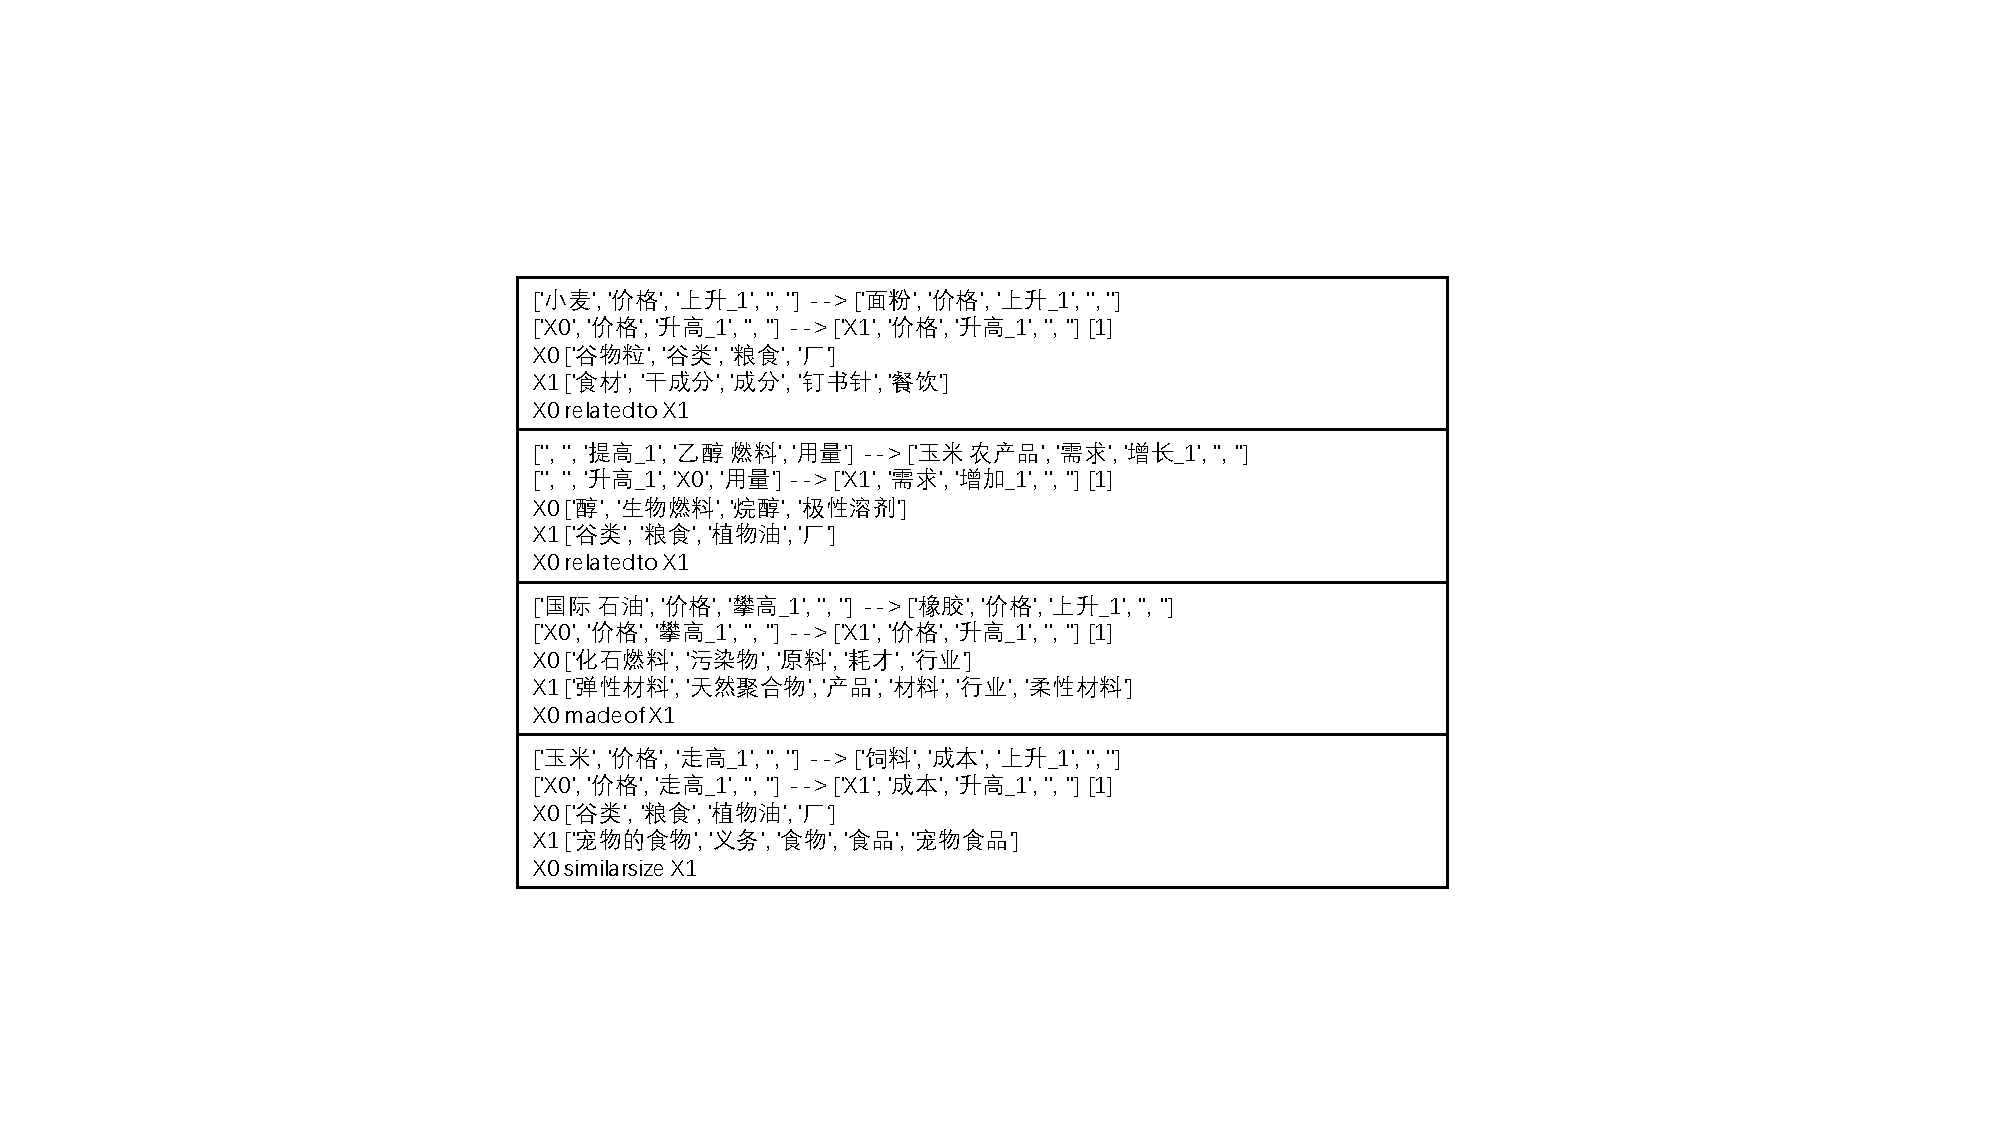
\includegraphics[width=0.95\columnwidth]{figures/reasonable_rule_case}
%	\end{center}
%	\caption{Examples of reasonable Rules.}
%	\label{fig:reasonable_rule_case}
%	\end{figure}
\begin{figure}[htbp]
	\centering
	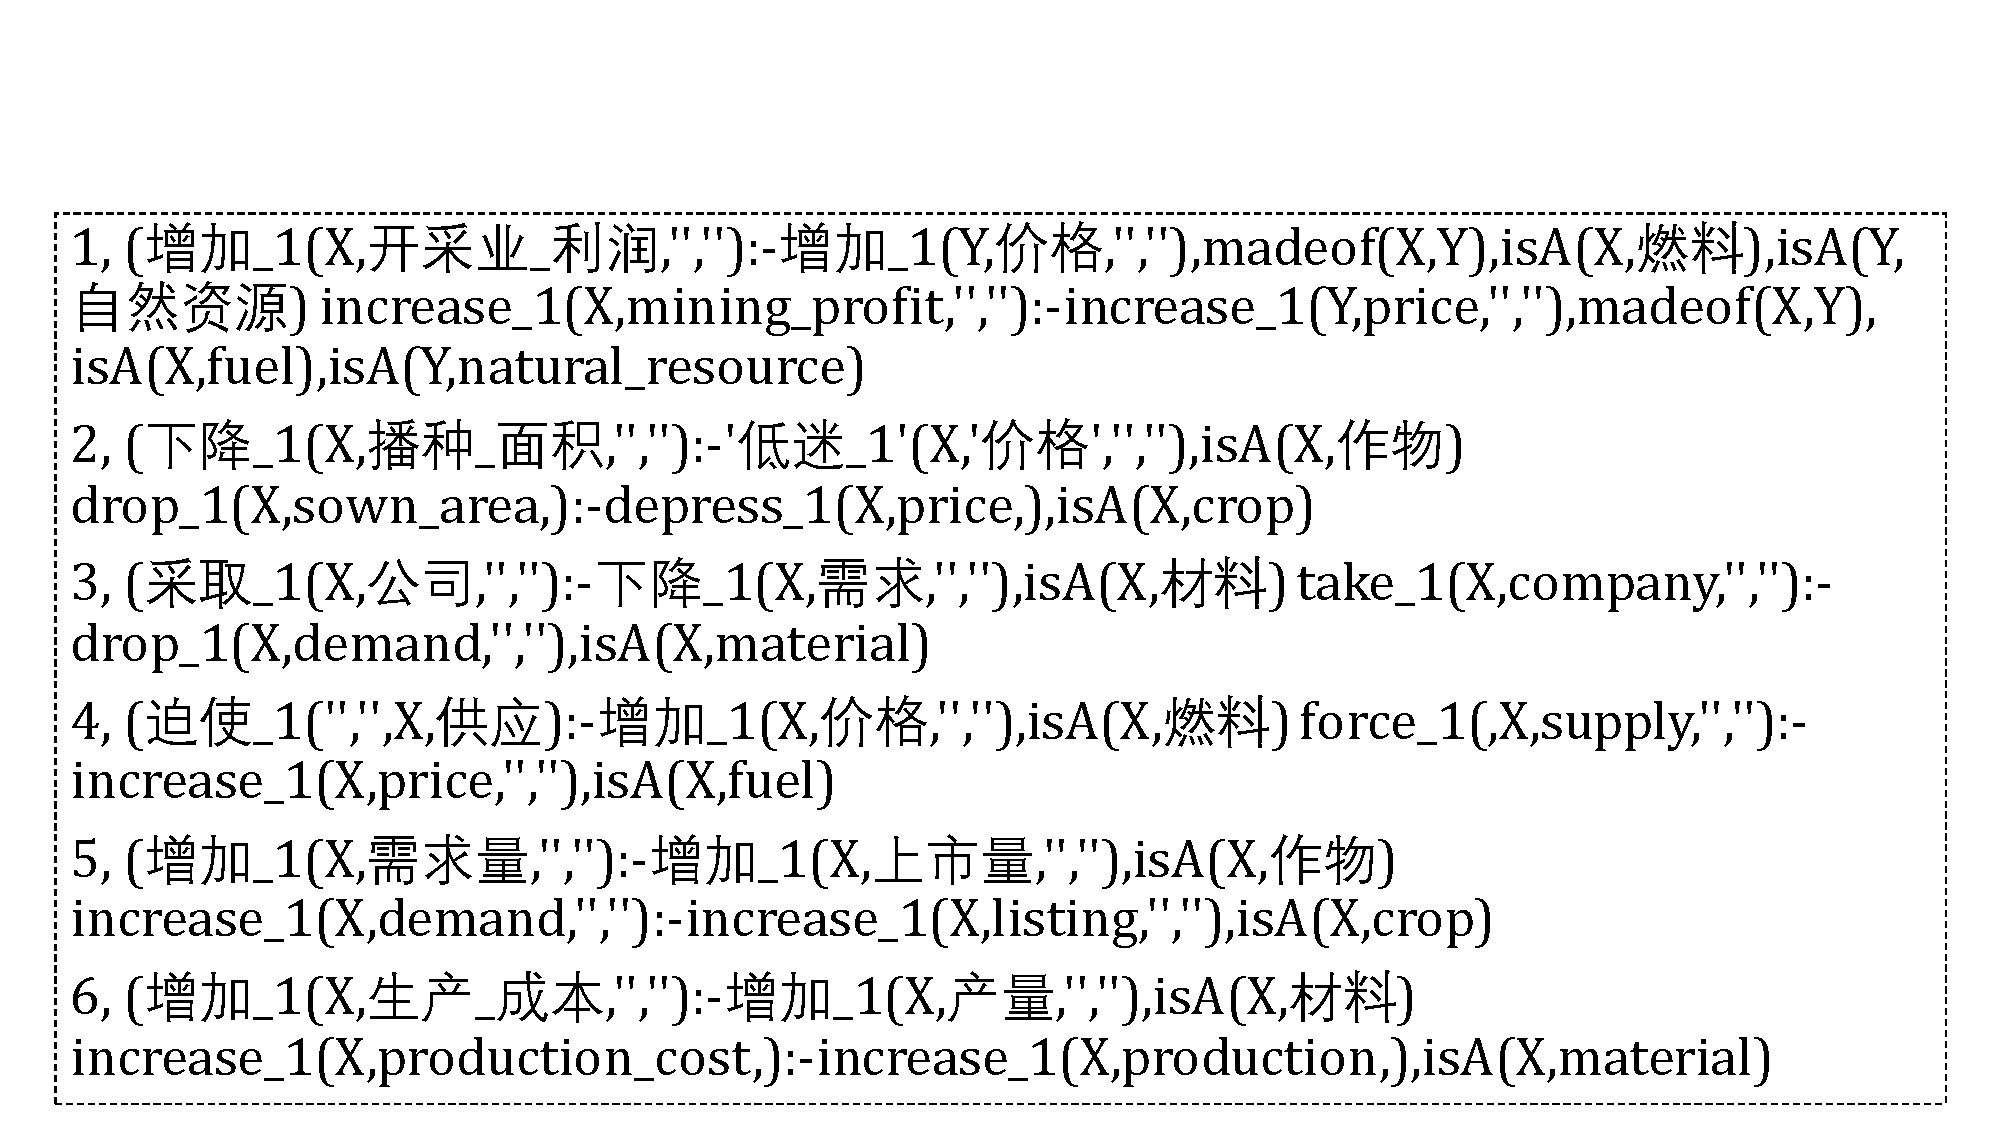
\includegraphics[width=0.95\columnwidth]{figures/rules_case}
	\caption{Examples of Typical Rules}
	\label{fig:rules_case}
\end{figure}
\paragraph{Event Graph}
With these rules, we deduce many rule instances with Prolog and pick out a tiny subgraph about rise and fall events, in Figure\ref{fig:rule_instantiation_graph}, to show the power of the rules. 
	
\begin{figure}[htbp]
\begin{center}
	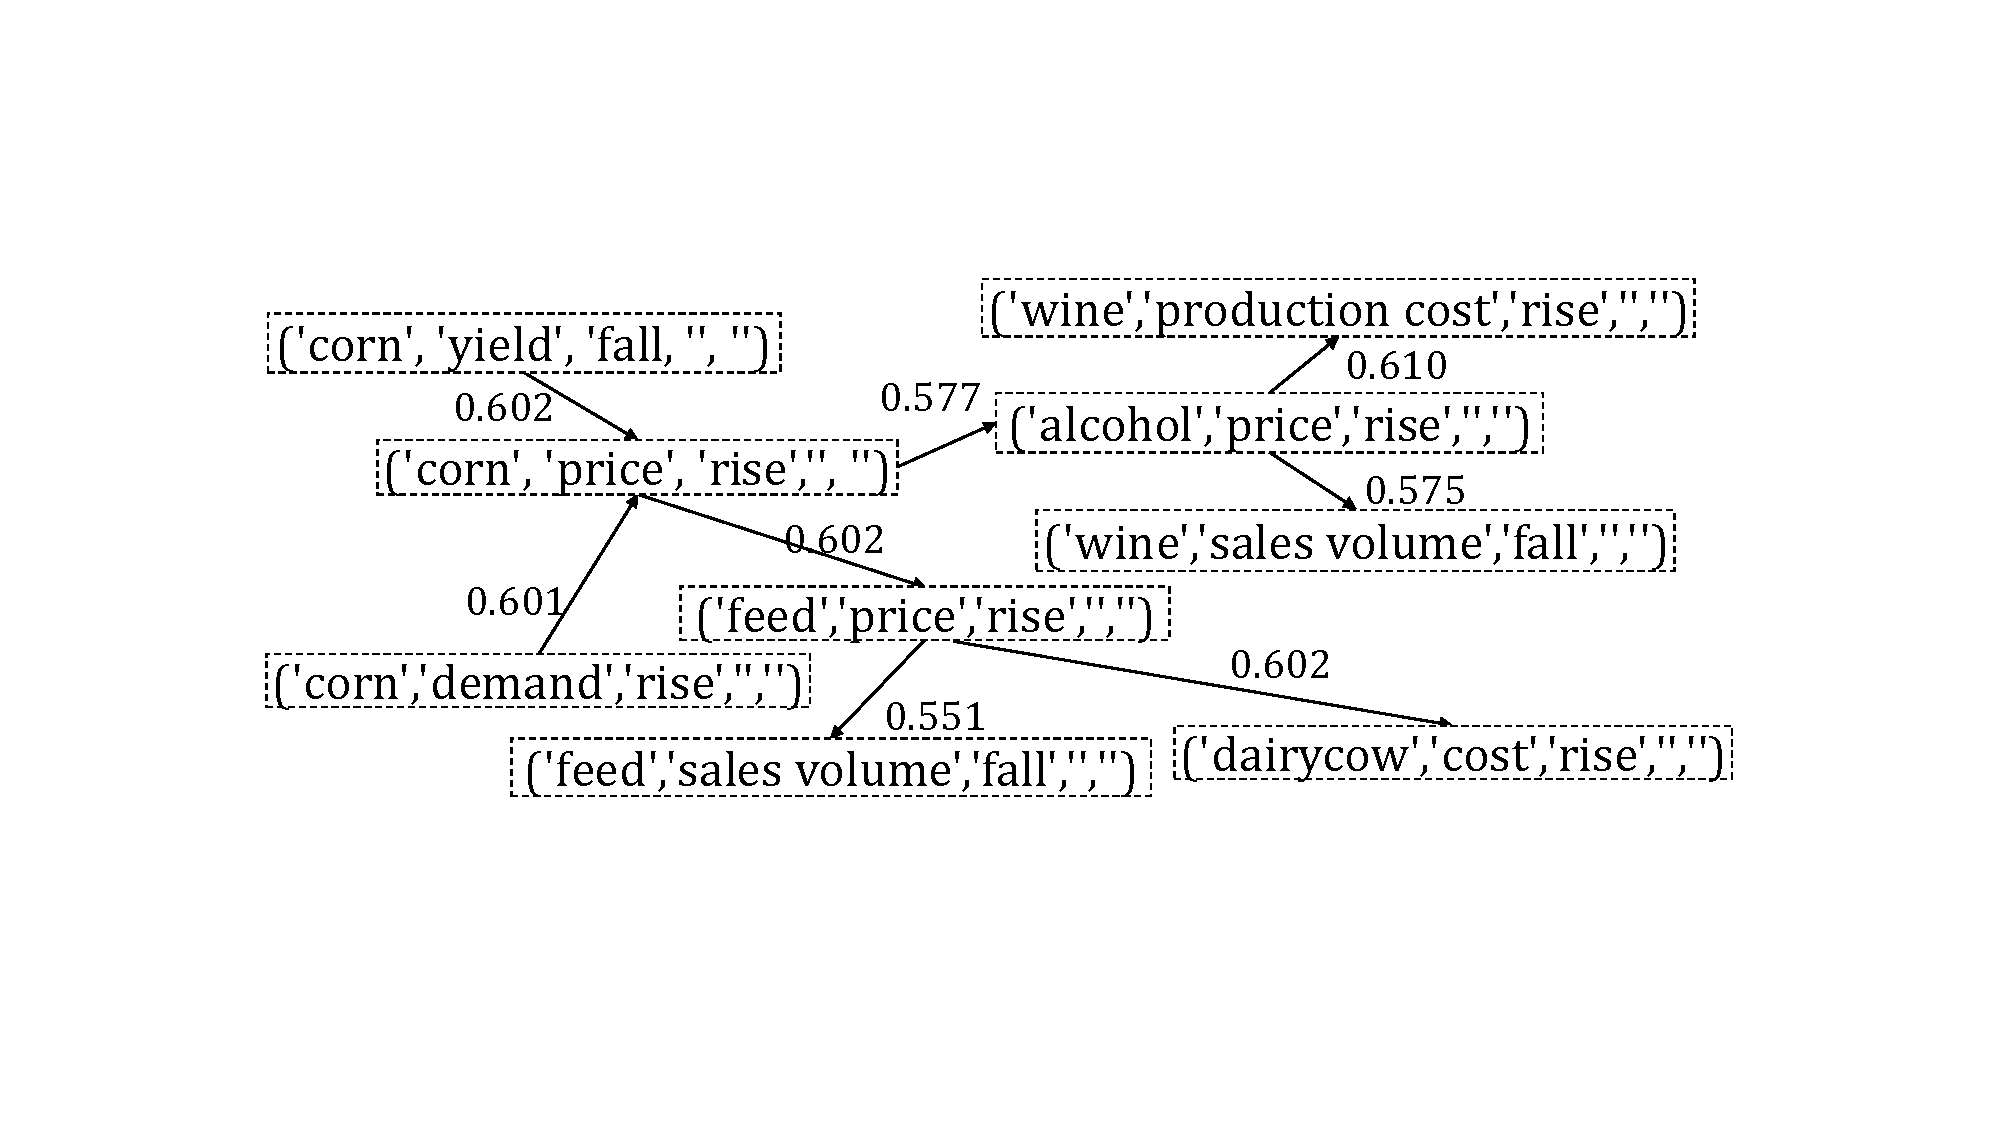
\includegraphics[width=0.9\columnwidth]{figures/instantiation_graph}
\end{center}
\caption{Rule Deduction. As space is limited, we only show the English version and omit the rules used in the reasoning process.}
\label{fig:rule_instantiation_graph}
\end{figure}

\subsection{Comparison with existing Knowledge Bases}
We compare our rules with causal part of other knowledge bases in various aspects in Table \ref{tab:comparison_rule_with_kbs}. We can see our causal knowledge representation is more expressive and informative, and the automatic knowledge acquisition is very convenient.
\begin{table*}[htbp]
\centering
%\begin{tabularx}{\columnwidth}{|c|c|c|c|}\hline
	\begin{tabular}{|c|c|c|c|c|c|c|c|}\hline
	\textbf{Name}&\textbf{Number}&\textbf{Domain}&\textbf{Unit}&\textbf{Data Structure}&\textbf{Information}&\textbf{Source}&\textbf{Precision}\\ \hline
	CausalNet&\textbf{62,675,002}&\textbf{Open}&word&(-)&rich&\textbf{automatic}&-\\
	\multicolumn{8}{|c|}{(`drink',`accident',36)}\\\hline
	ConceptNet &89,416&\textbf{Open}&short text&unstructured&rich&crowdsourcing&\textbf{100\%}\\
	\multicolumn{8}{|c|}{(`smoking',`/r/Causes',`cancer')}\\\hline
	FrameNet&59&\textbf{Open}&frame&\textbf{structured}&richer&crowdsourcing&\textbf{100\%}\\
	\multicolumn{8}{|c|}{Killing(Killer,Place,Means,Victim,Instrument),CausativeOf,Death(Protagonist,Place,Manner,Time)}\\\hline
	ATOMIC&568,312&\textbf{Open}&\textbf{logic event}&semi-structured&much richer&crowdsourcing&86.2\%\\
	\multicolumn{8}{|c|}{If ``PersonX pays PersonY a compliment", Then ``PersonY will smile"}\\\hline
	Ours&50,000&Finance&\textbf{logic event}&\textbf{structured}&\textbf{richest}&\textbf{automatic}&32.5\%\\ 
%			Deductive Rule Instance&\TD{??}\\ 
%	\multicolumn{8}{|c|}{See above rule example in Figure\ref{fig:rules_case}}\\\hline
\multicolumn{8}{|c|}{(Z,`price',`rise',`',`'):-(`',X,`suffer',Y,`attack'),isA(X,`country'),isA(Y,`disaster'),isA(Z,`metal'),atLocation(Z,X) conf:0.842}\\\hline	
	\end{tabular}
%\end{tabularx}  \cite{sap2018atomic}
\caption{Comparison with existing knowledge bases}
\label{tab:comparison_rule_with_kbs}
\end{table*}



%\begin{table}[htbp]
%	\caption{Rule Instance \& Rule}
%	\begin{center}
%	\begin{tabular}{|r|l|}\hline
%		\multicolumn{1}{|c|}{Name}                  & \multicolumn{1}{c|}{Number} \\\hline
%		\multicolumn{1}{|c|}{Rule Instances}        & \multicolumn{1}{c|}{7835403} \\ \hline
%		\multicolumn{1}{|c|}{Rules}                 & \multicolumn{1}{c|}{69036}  \\ \hline
%		\multicolumn{1}{|c|}{more than on relation} & \multicolumn{1}{c|}{2499(3.6\%)}\\
%		\multicolumn{1}{|c|}{only one relation}     & \multicolumn{1}{c|}{66539(96.4\%)} \\
%		\hline
%		==                                          & 56449(84.8\%)                      \\
%		madeof                                      & 5659(8.5\%)                        \\
%		atlocation                                  & 1835(2.76\%)                       \\
%		partof                                      & 1061(1.59\%)                       \\
%		usedfor                                     & 954(1.43\%)                        \\
%		hasa                                        & 511(0.768\%)                       \\
%		derivedfrom                                 & 38(0.0571\%)                       \\
%		hasproperty                                 & 20(0.0301\%)                       \\
%		createdby                                   & 12(0.018\%)                        \\ \hline
%	\end{tabular}
%	\label{tab:rule_statistics}
%\end{center}
%\end{table}
	%Rule Instances & 1817014(4337755)\\
	%Candidate Rules & 86218(201359)\\
	%Rule & 18348(42246)\\

\subsection{Ablation Study}
In this section, we explore the contributions of the various components of our rule learning framework.
\paragraph{Causal patterns statistic} The matched sentences distribution over 3 groups of patterns is shown in Table \ref{tab:pattern_statistics}. All patterns in one group have different causal cue words literally but the same meaning. It shows the third pattern group is more rigorous than the first two groups but has lower usage. Probably because more logical thinking is needed when editing news using more rigorous patterns.

%		\begin{table}[htbp]
%		\caption{Causal patterns. A is a cause tokens span, and B is an effect tokens span. Word '因为' represents a group works like '由于,'是因为','因为','缘于','归因于','原因是','起因','鉴于', and word '所以' represents a group of words like '所以','因而','因此','故此','故而','因故','导致','招致','以致','引致','诱致','致使','造成','使得','从而','从而使','于是','为此'}
%		\begin{center}
%			\begin{tabular}{|c|c|} \hline
%				\textbf{Pattern}& \textbf{Priority}\\ \hline
%				因为 A, 所以B&1\\ \hline
%				A,所以 B&2\\ \hline
%				因为 A,B&3\\ \hline
%			\end{tabular}
%			\label{tab:causal_pattern}
%		\end{center}
%	\end{table}	
	
\begin{table}[htbp]
	\centering
	\begin{tabular}{|c|c|c|c|} \hline
		\textbf{Pattern template}& \textbf{Priority}&\textbf{Number}& \textbf{Rate}\\	\hline 
		因为 A,B&1&2000242&48.32\% \\ \hline 
		A,所以 B&2&1530311&36.96\% \\ \hline 
		因为 A, 所以B&3&576851&14.72\% \\	\hline
	\end{tabular}
	\caption{Number of sentences extracted by causal patterns. A is a cause span and B is an effect span. Word `因为' represents a group works like 由于,是因为,因为,缘于,归因于,原因是,鉴于, and word `所以' represents a group of words like 所以,因而,因此,故而,因故,导致,招致,以致,引致,诱致,致使,造成,使得,从而使,于是,为此}
	\label{tab:pattern_statistics}
\end{table}	
\paragraph{External Knowledge Bases}
The following is some statistics of external knowledge bases used in the rule learning framework. The size of the lexicon is 12,624, obtained from `Industrial classification for national economic activities'\footnote{\url{ http://www.stats.gov.cn/Tjsj/tjbz/hyflbz/}}, which determines which event role in the rule instance can be generalized. 
To our knowledge, most existing Chinese taxonomic knowledge bases, such as CN-Probase\cite{Xu2017}, zhishi.me\cite{Niu2011}, are constructed from online-encyclopedia, which suffer that the concepts inside are far less than Probase and they have no probabilistic character. So we translate Probase to get 11,292,493 Chinese `IsA' pairs.
To our knowledge, there exists no large-scale Chinese commonsense knowledge base, so we translate the English part of ConceptNet and merge the Chinese part to get 2,085,681 Chinese triples.
We randomly sample 500 items from translated Probase and ConceptNet, respectively, and the accuracies after the human evaluation are \textbf{87.8\%}(close to the accuracy of original Probase 92.6\%) and \textbf{91.6\%}.

%\begin{table}[htbp]
%	\centering
%	\begin{tabular}{|c|c|}\hline
%		\textbf{Name}&\textbf{Number}\\ \hline
%		Lexicon&12624\\ \hline
%		Translated Probase &11,292,493(87.8\%)\\ \hline
%		Translated ConceptNet&2,085,681(91.6\%)\\ \hline
%	\end{tabular}
%	\caption{External Knowledge Bases}
%	\label{tab:knowledge_base_statistics}
%\end{table}

%After translation, the number of Chinese IsA pairs is 11,292,493. The number of Chinese commonsense triples is 2,085,681. We both randomly sample 500 items from them, and the accuracy after human evaluation are 0.878 and 0.916 respectively.
%The accuracy of original Probase is 0.926. 
%The number of total Chinese IsA pairs are 11,292,493 which contain concept-instance pairs and concept-subconcept pairs, the. The number of Chinese concepts is 81082 concluding concepts and subconcepts. The number of instances is 158693. The number of Chinese commonsense pairs is 7316977.
%\subsection{External Factual Knowledge Bases}

%From above rule instance extraction submodule, we scan get a rule instances repository. With such huge specific rule instances, we hope to further discover the powerful knowledge hidden in these rule instances. 

%so we generalize such a large amount of rule instances with a more general form. As discussed in Section \ref{sec:intro}, we need to build such a knowledge base. Taxonomy and common sense are two major kinds of knowledge in such knowledge base.
%In our framework, we need to rely on the external Chinese knowledge bases, Chinese Probase and Chinese Conceptnet, to generalize rule instances and add constraints. Most existing Chinese taxonomy knowledge is constructed from online-encyclopedia, such as CN-Probase\cite{Xu2017}. They usually focus more on named entity such as famous movie stars, singer stars, while we care more about the concrete things existed in life such as corn, steel, alcohol and so on.  In addition, they have no probabilistic character. Translation is an effective and efficient approach, we choose to translate Probase, which is a probabilistic taxonomic knowledge base.
%To our knowledge, there exists no large-scale Chinese commonsense knowledge base, so we translate the English part of ConceptNet5 into Chinese and combine the Chinese part.

%	 which is special for this, But it is only for English. We have investigated the CN-Probase\cite{xu2017cn}, but It even can't find the concept of common entities like '中国/China', '橡胶/rubber' and it also limits the usage frequency. So we collect the items from Probase, the items with 'IsA' relation in ConceptNet5\cite{speer2013conceptnet}, Webbrain\cite{chen2016webbrain}. Then, we fuse them together, Then, translate them into Chinese with google translator. to reduce the translate error, we put more context into the translator as more as possible, for example we put 'fruit such as apple, banana', Then we can get the translated result of IsA(apple,fruit), IsA(banana, fruit) together, which can make word sense of 'apple' to be translated near the fruit not company.  
%	\subsubsection{Chinese Commonsense knowledge base.}
%	, consisting of 47, 3, 25 relations respectively. Some of them are duplicative and some are useless for us. So we select specific number useful relations and we also design some patterns to extract some relations from Chinese wiki. 
%	relattions between arguments are used in rule specialization submodule to make rules reasonable. There exist many commonsense knowledge bases such as ConceptNet5, WebBrain, WebChild.  The numbers of the relations in these knowledge bases are limited. And some relations are equivalent among different knowledge bases, such as '/r/RelateTo' in ConceptNet is equivalent to 'relateto' in WebBrain. So we normalize all the relations names literally.
% Meanwhile, many pairs of arguments have more than one relations which are  duplicated semantically. For example, (sweet corn, corn) has the relations 'relatedto' and 'partof', obviously, 'partof' consists of 'relatedto' semantically. So we hope to remove the semantic reduplication relations. which means we need find the semantic containment relations among these relations.
%Algorithm \ref{alg:alg1} shows the Relations Containment algorithm we proposed. It firstly counts each relation and its corresponding arguments pairs. Then, compare the every two correlated relations, and record their containment relation. Last, enumerate all relations in each pair of arguments, remove the relation which is not contained in other relations existed in this pair of arguments.
%When fusing these knowledge bases, we regard arguments from different knowledge bases which have the same literal name as the same arguments.
%	from structured information to knowledge which is close to intelligence
%The goal of rule acquisition is to learn first-order logic rule from huge number of rule instances with the support of external factual knowledge, shown in the Figure \ref{fig:overview}'s middle part.
%with the knowledge base, now, we can generalize the rule instances extracted from rule instances extraction submodule into candidate rules to represent more general knowledge. For example, we hopefully generalize from each cluster of rule instances to one candidate rule. For example, given two rule instances in one cluster, ('国际 石油', '价格', '攀高@攀高', '', '') $->$ ('橡胶', '价格', '上升@升高', '', '') and ('国际 柴油', '价格', '攀高@攀高', '', '') $->$ ('橡胶', '价格', '上升@升高', '', ''), the generalized candidate rule would be('X0', '价格', '攀高', '', '') $->$ ('X1', '价格', '升高', '', '') where 'X0' IsA' 化石燃料','原料' and  'X1' IsA '弹性材料' '天然聚合物'.


%\begin{table}[htbp]
%\centering
%		\begin{tabular}{|c|c|}\hline
%			\textbf{Name}&\textbf{Number}\\ \hline
%			Lexicon&12624\\ \hline
%			Concepts &18281\\	
%			IsA pairs &123547\\
%			Concept-subconcept pairs&18753\\
%			Concept-instance pairs&104794\\\hline
%			Commonsense Pairs&32593\\ 
%			Commonsense Relations&10\\ \hline
%		\end{tabular}
%		\caption{Knowledge Base}
%		\label{tab:knowledge_base_statistics}
%\end{table}
\paragraph{Open Event Extraction}
%	TextRunner/WOE,ReVerb,Ollie,ClausIE,SRL/AMR parsing/frame-semantic parsing,NestIE 
Since our event structure scheme is plain and straightforward, we choose the reliable Stanford CoreNLP tool to extract the rule instances.
%	rule instance  97/200(48.5\%)& 21/200(10.5\%) & 82/200(41.0\%) \\ \hline
The number of rule instances extracted after rule instance distilling submodule is 7,835,403. Since most of them are discarded in the learning process, the number of rule instances really used for rule induction is 78,098 with an accuracy of \textbf{48.5\%} (we also sample 200 rule instances and manually evaluate them).

%\textit{To sum up}, our framework is a pipeline, in which rule instance extraction achieve 48.5\%, ConceptNet5 translation achieve 91.6\% and Probase translation achieves 87.8\%, So teh rule finally can achieve 39.0\%(48.5\%*91.6\%*87.8\%) maximumly, which is close to the evaluation of the final rules. 

%\textbf{\textit{To sum up}}, 
%our framework is a pipeline, in which the accuracy of rule instance extraction is 48.5\%, the accuracy of ConceptNet5 translation is 91.6\%, and the accuracy of Probase translation is 87.8\%. 
\textbf{\textit{To sum up}}, our framework is a pipeline undergoing rule instance extraction(accuracy 48.5\%), constrain relations addition(accuracy of ConceptNet 91.6\%), and rule induction(accuracy of Probase 87.8\%).
Thus, the accuracy can only reach \textbf{39.0\%} (48.5\%*91.6\%*87.8\%) at the maximum, which is close to our evaluation(32.5\%) of the final rules.

%	\subsubsection{Rule Acquisition}
%	\begin{table}[]
%		\centering
%		\begin{tabular}{lll}
%			& rule number  & qualitity       \\
%			no Coneptnet / only one relation    & 66539/96.4\% & informative     \\
%			Conceptnet / more than one relation & 2499/3.6\%   & more infrmative
%		\end{tabular}
%		\caption{Relation Number}
%	\end{table}

%	\begin{table}[]
%		\caption{Event Connection}
%		\begin{center}
%		\begin{tabular}{lll}
%			==         & 60475 & 84.4\%  \\
%			madeof     & 6161  & 8.6\%   \\
%			atlocation & 2104  & 2.94\%  \\
%			partof     & 1152  & 1.61\%  \\
%			usedfor    & 1072  & 1.5\%   \\
%			others     & 674   & 0.941\%
%		\end{tabular}
%		\end{center}
%	\end{table}
\subsection{Application: Futures Price Prediction}
%\paragraph{Reasoning with Uncertainty}
\begin{figure}[htbp]
	\begin{center}
		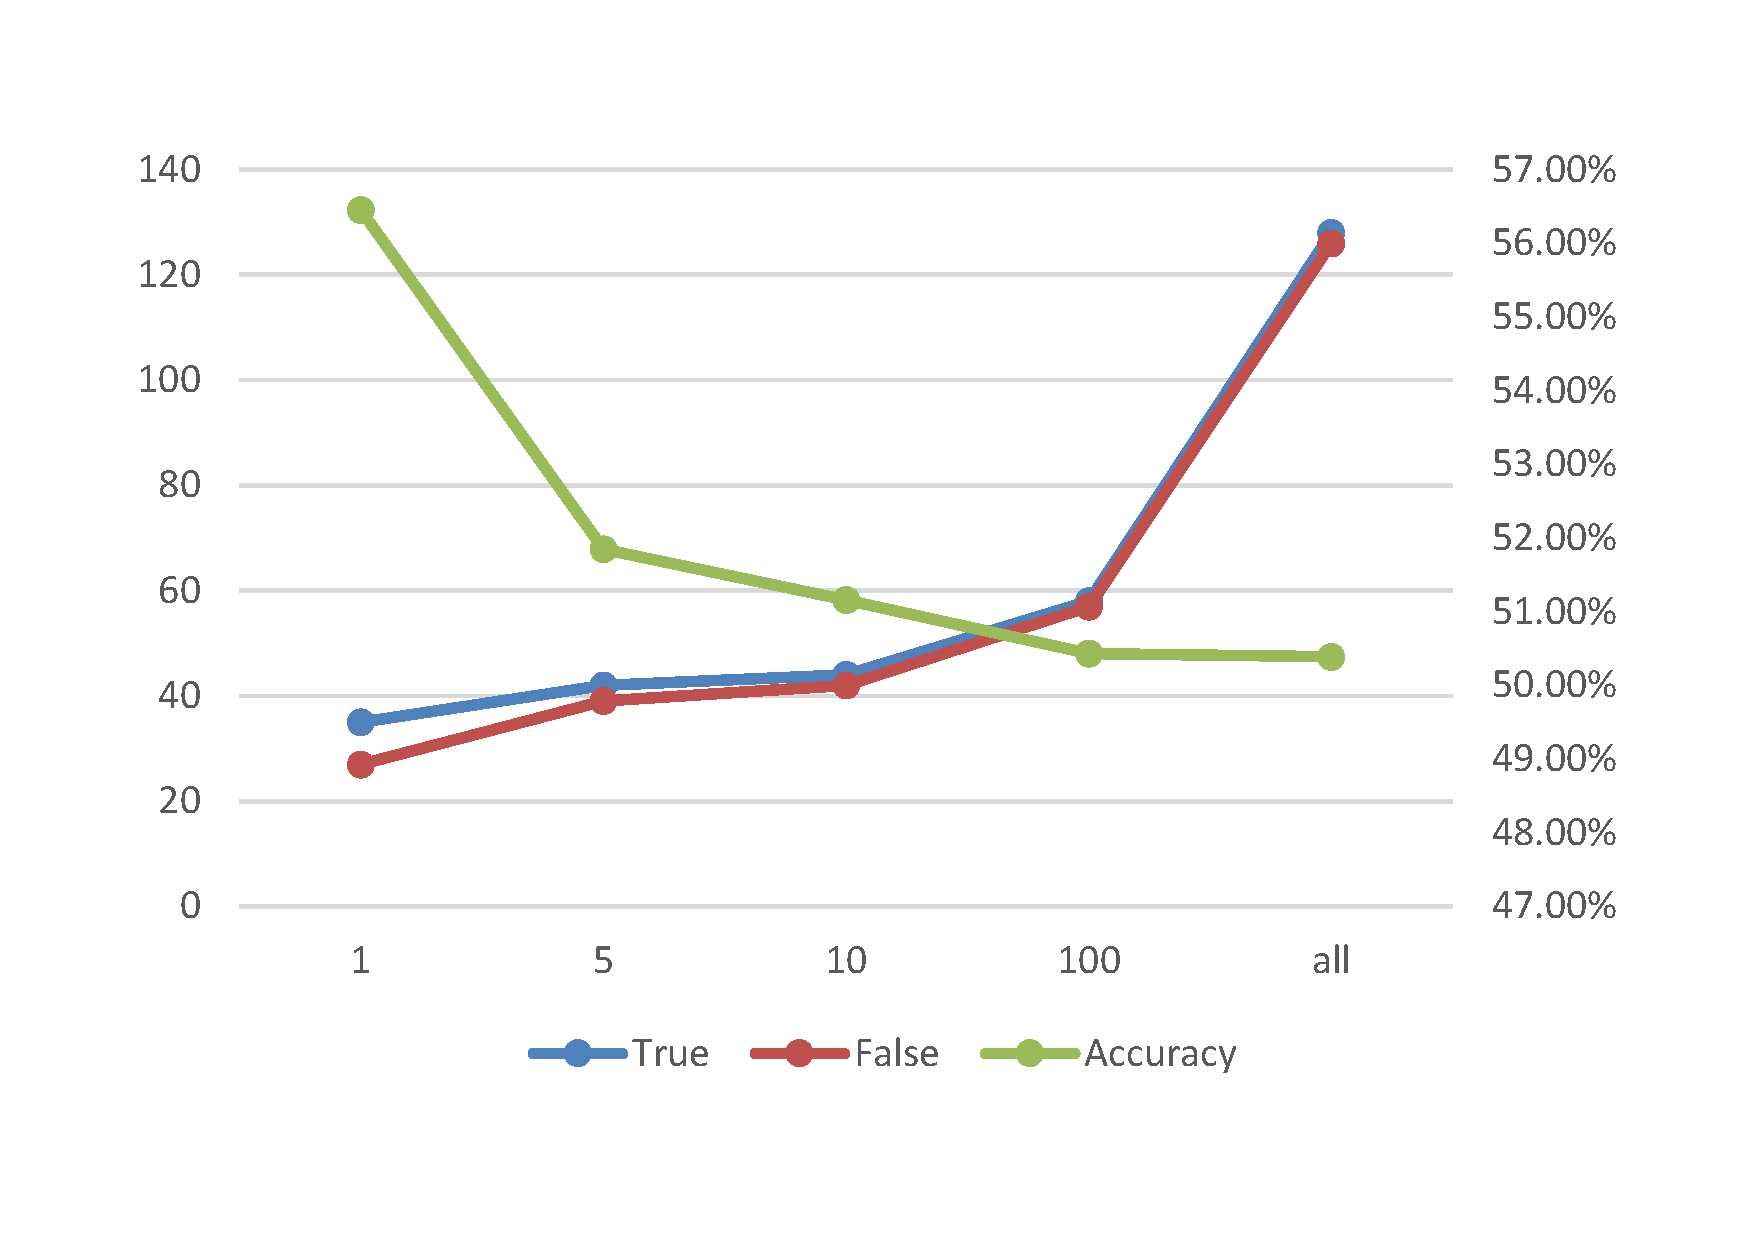
\includegraphics[width=0.9\columnwidth]{figures/rule_futures_prediction}
	\end{center}
	\caption{Futures Price Prediction.}
	\label{fig:futures_price_prediction}
\end{figure}
We choose futures price prediction because the futures are common and concrete things existed in ConceptNet and Probase, such as corn, oil, etc.
%\cite{Ding} is the state-of-the-art stock prediction model(EB\_CNN). We follow similar experimental settings. 
We follow similar experimental settings in \cite{Ding}.
From 2018/1/1 to 2018/11/2, we collect all the headlines and the price change of 15 futures as test data, which include \textbf{851} price change events (The price change of more than 1\% relative to the previous day is an event and we only focus on rise or fall events). 

Baseline models: EB\_CNN model \cite{Ding}, the state of the art model in stock price prediction, uses a deep convolutional neural network to model both short-term and long-term influences of events on stock price movements, and the accuracy of futures prediction is \textbf{54.2\%}. Other models in \cite{Ding}, such as EB\_NN, WB\_CNN, and WB\_NN can achieve \textbf{53.0\%}, \textbf{53.2\%}, and \textbf{53.5\%}, respectively. These accuracies of futures prediction are lower than the accuracies of stock prediction shown in the paper.
It may be because the factors affecting the futures price are far less than the stock price and the futures price is much more stable than the stock price, which makes useful training information about the futures less and further affects the accuracy of the models.

Our approach: For each actual future price change event , we get the news headlines for the previous month before this event. 
For each news headline, we extract the event, use Prolog to reason based on the rules and external knowledge bases, and get the top K inferred events sorted by the confidence.
We may have m*K inferred events for this event, m is the number of events occurred in this month. 
Here, we select the price change events(rise or fall) of the future in this actual future price change event from m*K events and calculate the weighted sum of their confidences(rise event weights 1 and fall event weights -1). If the sum value is positive, we predict this future price as a rise event, otherwise as a fall event. If get no related events changing the future's price, do not make prediction. We compare this prediction with the actual price change to evaluate the reasoning effect. 
Figure \ref{fig:futures_price_prediction} shows the average prediction result. It shows the more predicted events inferred from the Prolog(by increasing K) we use, the lower the prediction accuracy is(from \textbf{56.5\%} to \textbf{50.4\%}), and the more futures events we can predict(from \textbf{62} to \textbf{254}). 

\textbf{\textit{To sum up}}, our rule-based prediction approach can have a higher prediction accuracy (56.45\%) and better interpretation ability with a low recall rate, which is very practical in life.

%\begin{table}[htbp]
%	\caption{Baselines and Proposed Framework}
%	\begin{center}
%		\begin{tabular}{lll}\hline
%			& Acc & MCC \\\hline
%			WB-NN &  0.535 &     \\
%			WB-CNN&  0.532  &     \\
%			EB-NN &  0.530  &     \\
%			EB-CNN&  0.542   &     \\
%			Rule &     &    \\\hline
%		\end{tabular}
%		\label{tab:baselines_and_rule}
%	\end{center}
%\end{table}

\subsection{Downloading and Demo}
The translated Chinese Probase and ConceptNet and learned rules are available at URL.
We built a demo to demonstrate the reasoning process at URL. 
We also developed an application demo of futures prices change triggering that can monitor news from around the world in real time, find the news that may cause futures prices changes, and alert users. Visit URL.

\section{Related Work}
\paragraph{Clarification Question Generation} The concept of CQ can be naturally raised in a dialogue system where the speech recognition results tend to be erroneous so that we raise CQs for sanity check \citep{stoyanchev2014towards}, or the intents for a task is incomplete or ambiguous in a first short utterance and further CQs are needed to fill in the slots \citep{dhole2020resolving}. The concept is then extended to IR to clarify ambiguous queries \citep{aliannejadi2019asking}, and has been successfully put into practice \citep{zamani2020generating}. Other application areas including KBQA \citep{xu2019asking} and open-domain dialogue systems \citep{aliannejadi2020convai3}. CQGen can also be applied to help refine posts on websites like StackExchange \citep{Kumar_2020} and Amazon \citep{rao2019answer}. In this context, our work closely follows the research line of \citep{rao2018learning, rao2019answer, cao2019controlling}. \citet{rao2018learning} first adopted a retrieval-then-rank approach. They \citep{rao2019answer} then proposed a generation approach to train the model to maximize the utility of the hypothetical answer for the questions with GAN, to better promote specificity. \citet{cao2019controlling} propose to control the specificity by training on data with explicit indicator of specificity, but it requires additional specificity annotation. Towards the similar specificity goal, we adopted a different keyword-based approach. They also assume generating one question per context, which we claim is not sufficient to cover various possible information needs, and thus propose the task of the diverse CQGen.

\paragraph{Diverse Generation} The demand for diverse generation exists in many other fields~\cite{vijayakumar2018diverse, LiangZ18code, shen2019mixture}, and we've drawn inspirations from these literatures. For image captioning, we may use multiple descriptions for different focusing points of a scene. \textit{Diverse Beam Search} \citep{vijayakumar2018diverse} was proposed to broaden the searching space to catch such diversity by dividing groups in decoding and imposing repetition penalty between them. For machine translation, a context can be translated with different styles. \citet{shen2019mixture} thus proposed \textit{Mixture of Expert} models including hMup to reflect various styles with a discrete latent variable (\textit{expert}). And here for CQGen, diversity is required to cover various potentially missing aspects, so we come up with the idea to use keywords as a controlling variable like \textit{expert} to promote diversity.



\section{Conclusion}

In this paper, we incorporated the idea of Cookie Theft picture description task into the evaluation of the high-level cognitive abilities of LVLMs and designed a novel evaluation benchmark called CogBench.
% Images in CogBench are of high quality and require more cognitive reasonings to understand, which makes it different from existing image datasets.
The images in CogBench are of high quality and demand more complex cognitive reasoning for interpretation, setting it apart from existing image datasets.
% It consists of a image description task and a VQA task.
Experiments show that there is still a large gap between the cognitive abilities of LVLMs and human beings, indicating CogBench is a challenging benchmark.

% In the future


%\acks
%
%Acknowledgments, if needed.

% We recommend abbrvnat bibliography style.

%{\renewcommand{\baselinestretch}{0.9}
%\small
\bibliographystyle{abbrvnat}
\bibliography{ocp,gcc}
%}

\appendix
\begin{minipage}{\textwidth}

\section{Rules of Different Commit Semantics}\label{sec:commits}

\subsection{Localized Commit}

\[
  \label{rule:localized-commit}
  \frac{
    [\cm.e,f]=A[i] \qquad
    (1\le i\le |A|)
  }
  {G\oplus_i\langle A,d,s\rangle \gto \langle A[i\mapsto[e,f]],d,\snapshot(s,|e|,i,f(d))\rangle}
\]

\subsection{Absolutely Eager Commit}

\[
  \label{rule:abs-eager-commit}
  \frac{
    w\in leaves(G) \qquad
    w=\langle A,d,s\rangle \qquad
    [\cm.e,f]=A[i] \qquad
    i\not\in cid(G) \qquad
    (1\le i\le |A|)
  }
  {G\oplus_i G' \gto \langle A[i\mapsto[e,f]],d,\snapshot(s,|e|,i,f(d))\rangle}
\]

\subsection{Eager Commit}

\[
  \label{rule:eager-commit}
  \frac{
    w\in leaves(G) \qquad
    w=\langle A,d,s\rangle \qquad
    [\cm.e,f]=A[i] \qquad
    i\not\in cid(G) \qquad
    w'=\langle A[i\mapsto[e,f]],d,\snapshot(s,|e|,i,f(d))\rangle \qquad
    (1\le i\le |A|)
  }
  {G\oplus_i G' \gto replace(G,w,w')}
\]

\subsection{Late Commit}

\[
  \tag{\sc Fork}
  \frac{
    {[(e_1\oplus e_2).e,f]=A[i]}\qquad
    {(1\le i\le |A|)}}
  {\langle A,d,s\rangle \gto
    \langle A[i\mapsto[e_1.e,f]],d,s\rangle^{\color{red} 1} \oplus_i
    \langle A[i\mapsto[e_2.e,f]],d,s\rangle^{\color{red} 2}}
\]

\subsection{Coordinated Commit}

\[
  \label{rule:eager-commit}
  \frac{
    \widetilde{G}=same(G,i,\cm) \qquad
    \widetilde{G}\neq\,\uparrow\fbox{\small undefined} \qquad
    i\not\in cid(G)
  }
  {G\oplus_i G'\gto\widetilde{G}}
\]

\[
  \frac{}
  { same(G_1\oplus_k G_2,i,e) = same(G_1,i,e)\oplus_k same(G_2,i,e) }
\]
\[
  \frac{
    w = \langle A,d,s\rangle \qquad
    [e.e',f]=A[i] \qquad
    (1\le i\le |A|)
  }
  { same(w,i,e) = \langle A[i\mapsto[e',f]],d,\snapshot(s,|e'|,i,f(d))\rangle }
\]

\end{minipage}


\end{document}
